%%%%%%%%%%%%%%%%%%%%%%%%%%%%%%%%%%%%%%%%%
% Beamer Presentation
% LaTeX Template
% Version 1.0 (10/11/12)
%
% This template has been downloaded from:
% http://www.LaTeXTemplates.com
%
% License:
% CC BY-NC-SA 3.0 (http://creativecommons.org/licenses/by-nc-sa/3.0/)
%
%%%%%%%%%%%%%%%%%%%%%%%%%%%%%%%%%%%%%%%%%

%----------------------------------------------------------------------------------------
%	PACKAGES AND THEMES
%----------------------------------------------------------------------------------------

\documentclass{report}
\pagestyle{plain}

\usepackage{graphicx} % Allows including images
\usepackage{booktabs} % Allows the use of \toprule, \midrule and \bottomrule in tables
\usepackage{blkarray} % Allows the use of labelled matrices
\usepackage{amsmath,amsfonts,amssymb}
\usepackage{mathtools}
%\usepackage[plain]{algorithm}
\usepackage{algorithm}
\usepackage[noend]{algpseudocode}

\usepackage[utf8]{inputenc}
\usepackage[english]{babel}
\usepackage{amsthm}

\usepackage{subcaption}
%\usepackage[demo]{graphicx}
%\usepackage{tikz,pgfplots} 

% set margins
\usepackage[margin=1.0in]{geometry}

\newtheorem{theorem}{Theorem}[section]
%\newtheorem{corollary}{Corollary}[theorem]
\newtheorem{corollary}[theorem]{Corollary}
\newtheorem{lemma}[theorem]{Lemma}
\newtheorem{definition}{Definition}[section]
%\newtheorem{definition}[theorem]{Definition}


\graphicspath{{../figs/}}

\usepackage{color}
%\usepackage{hyperref}       
%\usepackage{varioref}       
%\usepackage{cleveref}
\usepackage[colorlinks=true, allcolors=blue]{hyperref}


% declaration of the new block
\algblock{ParFor}{EndParFor}
% customising the new block
\algnewcommand\algorithmicparfor{\textbf{parallel for}}
\algnewcommand\algorithmicpardo{\textbf{do}}
\algnewcommand\algorithmicendparfor{\textbf{end parfor}}
\algrenewtext{ParFor}[1]{\algorithmicparfor\ #1\ \algorithmicpardo}
\algrenewtext{EndParFor}{\algorithmicendparfor}

% supprese EndParFor
\makeatletter
\ifthenelse{\equal{\ALG@noend}{t}}%
  {\algtext*{EndParFor}}
  {}%
\makeatother


\newcommand{\push}[1]{\text{push} \left ( #1 \right )}
\newcommand{\pop}{\text{pop}()}

\DeclareMathOperator*{\argmax}{arg\,max}
\DeclareMathOperator*{\argmin}{arg\,min}

\newcommand{\algoname}[1]{\textnormal{\textsc{#1}}}

\newcommand{\E}{\mathbb{E}}
\newcommand{\Var}{\mathrm{Var}}
\newcommand{\Cov}{\mathrm{Cov}}
\newcommand{\Bias}{\mathrm{Bias}}
\newcommand{\med}{\mathrm{median}}
\newcommand{\mean}{\mathrm{mean}}
%\newcommand{\argmax}{\mathrm{argmax}}
%\newcommand{\argmin}{\mathrm{argmin}}
\newcommand{\poly}{\mathrm{poly}}
\newcommand{\polylog}{\, \mathrm{polylog} \,}
\newcommand{\el}{\mathrm{else}}
\newcommand{\diag}{\mathrm{diag}}
\newcommand{\rank}{\mathrm{rank}}
\newcommand{\nnz}{\mathrm{nnz}}

%----------------------------------------------------------------------------------------
%	TITLE PAGE
%----------------------------------------------------------------------------------------

%\date{\today} % Date, can be changed to a custom date

\begin{document}

%\pagenumbering{gobble}
\pagenumbering{roman}

\begin{center}
\textbf{Sublinear Approximation of Centrality Indices in Large Graphs}
\vspace{0.4cm}
%\title{Sublinear Approximations of Vertex Importance in Evolving Social Network Graphs}

A Thesis \\
Submitted to the Faculty \\
in partial fulfillment of the requirements for the \\
degree of \\[0.4cm]
Doctor of Philosophy \\[0.4cm]
by\\[0.5cm]
Benjamin W. Priest\\[0.4cm]
Thayer School of Engineering \\
Dartmouth College \\
Hanover, New Hampshire \\[0.4cm]
June 2017 
\vspace{0.5cm}

\end{center}

Examining Committee:

\begin{flushright}
Chairman \line(180, 0){110} \\
George Cybenko\\[1cm]

Member \line(180, 0){110} \\
Eugene Santos\\[1cm]

Member \line(180, 0){110} \\
Amit Chakrabarti \\[1cm]

Member \line(180, 0){110} \\
Roger Pearce\\[1cm]

%(ALL signatures must be in Black ink, ALL fonts in black ink)

\end{flushright}

\begin{flushleft}
\line(180, 0){110} \\
F. Jon Kull, Ph.D.\\
Dean of Graduate and Advanced Studies\\[1cm]
%NOTE: the copies you submit must have the original signatures for PhD, one hard copy, for MS, one hard copy and a pdf of the thesis is required for both degrees.  No Holes, clips or binding on the copy and should be on Quality paper, preferably, Dartmouth Bond.
\end{flushleft}


%\author{Benjamin W. Priest}
%\affil{Dartmouth College, Thayer School of Engineering, Hanover, NH, USA}
%\affil{benjamin.w.priest.th@dartmouth.edu}
%\affil[b]{Affiliation2, Address, City, Country}



%----------------------------------------------------------------------------------------
 \pagebreak
 \null
 \pagebreak
%\pagenumbering{roman}
%----------------------------------------------------------------------------------------


\renewcommand{\abstractname}{Acknowledgements}
\begin{abstract}

I am priviledged to work with my advisor George Cybenko. 
The subject of this thesis would never have come to my attention without his prompting, and its contents would never have come to fruition without his guidance. 
George has been a patient mentor and a good friend.

I would like to thank Eugene Santos, Amit Chakrabarti, and Roger Pearce for agreeing to serve on my thesis committee, and for their time and guidance during the process.
I would like to thank Amit Chakrabarti in particular, who introduced me to the data stream model and changed the trajectory of my career in the process.

I have been fortunate to work with my excellent co-authors and colleagues 
Kate Farris, 
Luan Huy Pham, 
Massamilano Albanese,
Roger Pearce,
Geoffrey Sanders,
Keita Iwabuchi, 
Trevor Steil,
and 
Jordan Katz.
I would especially like to thank Roger Pearce and Geoffrey Sanders for their mentorship during my time at Lawrence Livermore National Laboratory. 

I must extend my sincere gratitude to Ellen Woerta for her administrative assistance, without whom I would have been lost and confused during much of my time at Dartmouth.

Finally, I would like to thank my friends and family for bearing with me and keeping me sane during this strange journey.
I appreciate especially everyone I called out of the blue to talk for hours about nothing in particular. 
It helped more that they can realize.
I would especially like to thank Ryan Andreozzi with whom I deadlifted 500 pounds, a milestone of which I am as proud as any of my academic achievements.

This thesis is dedicated to Jennifer Lay. 
Whatever my destination, I hope to travel with her.
\end{abstract}




\renewcommand{\abstractname}{Abstract}
\begin{abstract}
The identification of important vertices or edges is a ubiquitous problem in the analysis of graphs.
There are many application-dependent measures of importance, such as centrality indices (e.g. degree centrality, closeness centrality, betweenness centrality, and eigencentrality) and local triangle counts.
%However, the computation of such indices is usually expensive on large graphs. 
%Moreover, evolving graphs with edge insertions, updates, and deletions are prevalent in applications. 
Traditional computational models assume that the entire input fits into working memory, which is impractical for very large graphs.
Exact algorithms on very large graphs in practice hold the graph in distributed memory, where a collection of processors partition the graph.
Distributed graph algorithms must optimize communication in addition to execution time.
The data stream model is an alternative approach to large data scale that assumes only sequential access to the input, which is handled in small chunks.
Data stream algorithms use sublinear memory and a small number of passes and seek to optimize update time, query time, and post processing time.  

In this dissertation, we consider the application of distributed data stream algorithms to the sublinear approximation of several centrality indices and local triangle counts. 
We pay special attention to the recovery of \emph{heavy hitters} - the largest elements relative to the given index.

The first part of this dissertation focuses on serial graph stream algorithms.
We present new algorithms providing streaming approximations of degree centrality and a semi-streaming constant-pass approximation of closeness centrality.
%We present new algorithms providing a streaming approximation of degree centrality, a semi-streaming constant-pass approximation of closeness centrality, and a semi-streaming approximation of HITS on large collections of small graphs.
We achieve our results by way of counting sketches and sampling sketches.

The second part of this dissertation considers vertex-centric distributed graph stream algorithms.
We develop hybrid pseudo-asynchronous communication protocols tailored to managing communication on distributed graph algorithms with asymmetric computational loads.
We use this protocol as a framework to develop distributed streaming algorithms utilizing cardinality sketches.
We present new algorithms for estimating vertex- and edge-local triangle counts, with special attention paid to heavy hitter recovery.
We also utilize $\ell_p$ sampling sketches for the adjacency information of high degree vertices to boost the performance of the sampling of random walks and subtrees. 
We present hybrid exact-approximating distributed algorithms for sublinearly sampling random walks, simple paths, and subtrees from scale-free graphs. 
We use these algorithms to approximate  $K$-path centrality as a proxy for recovery the top-$k$ betweenness centrality elements.

%These constraints place us in what is sometimes called the turnstile or dynamic streaming model. 
%Randomized algorithms maintaining sketches of salient graph properties are known to allow approximation of some graph properties in sublinear space. 

%It is therefore desirable to develop sublinear algorithms to approximate centrality indices.
%It is in particular desirable to develop such algorithms that require only one pass over the input stream, although a provably small number of passes is also interesting in some cases. 
%In applications it is usually more important to recover the top $k$ central vertices with respect to a given index than it is to know the exact scores of every vertex in the network. 
%Accordingly, the relaxed problem of maintaining an on-line list of the approximate top $k$ central vertices is of primary interest, especially in the single-pass case.

%We provide a preliminary streaming approximation algorithm for degree centrality utilizing \algoname{CountSketch} as a proof of concept.
%We also discuss how existing graph sparsification algorithms provide an approximation to closeness centrality using loglinear space.
%This approach is also much faster that conventional algorithms in the case that the underlying graph is dense. 
%Finally, we provide an approximation for the HITS indices, a variant of eigencentrality, using low-rank approximation sketches. 

%We propose that these initial results are the tip of the iceberg, and that approximations to deeper and more widely-used centrality indices may be feasible.
%In particular, we discuss approximating the top betweenness central vertices by way of $\kappa$-path centrality, and how this approach may enable a sublinear approximation. 
%We also discuss the approximation of eigencentrality measures by way of low-rank approximation sketches on general matrices. 
%Although this methodology does not guarantee error bounds, it may still prove to be empirically useful. 

\end{abstract}

%\keywords{graph processing, evolving graphs, centrality, data stream model, sketching, pass-constrained algorithms}


\tableofcontents

%----------------------------------------------------------------------------------------
%----------------------------------------------------------------------------------------
\chapter{Introduction} \label{chap:intro}
%----------------------------------------------------------------------------------------
%----------------------------------------------------------------------------------------
\pagenumbering{arabic}



Many modern computing problems focus on complex relationship networks arising from real-world data. 
Many of these complex systems such as the Internet, communication networks, logistics and transportation systems, biological systems, epidemiological models, and social relationship networks map naturally onto graphs \cite{wasserman1994social}.
%These networks, sometimes labeled ``social networks'' due to their roots in human behavior, often exhibit similar structure and submit to similar analyses. 
A natural question that arises in the study of such networks is how to go about identifying ``important'' vertices and edges.
How one might interpret importance within a graph is contingent upon its domain.
Accordingly, investigators have devised a large number of importance measures that account for different structural properties. 
These measures implicitly define an ordering on graphs, and typically only the top elements vis-\'a-vis the ordering are of analytic interest.

However, most traditional RAM algorithms scale poorly to large datasets. 
This means that very large graphs tend to confound standard algorithms for computing various important orderings. 
Newer computational models such as the data stream model and the distributed memory model were introduced to address these scalability concerns.
The data steam model assumes only sequential access to the data, and permits a sublinear amount of additional working memory.
The time to update, query, and post process this data structure, as well as the number of passes and amount of additional memory are the important resources to optimize in the data stream model.
The data stream model is a popular computational model for handling scalability in sequential algorithms.
The distributed memory model partitions the data input across several processors, which may need to subsequently communicate with each other.
The amount of communication is an important optimization resource.
In practical terms, minimizing the amount of time processors spend waiting on their communication partners is also important.

Although both models have been applied to very large graphs independently, there is relatively little literature focusing on the union of the two models of computation. 
In this work we devise distributed data stream algorithms to approximate orderings of vertices and edges of large graphs. 
We focus in particular on recovering the heavy hitters of these orderings.
We consider the sublinear approximation of classic centrality scores, as well as local and global triangle counts.
We also describe space-efficient methods for sampling random walks and subtrees in scale-free vertex-centric distributed graphs, and their application to estimating some centrality indices.

%----------------------------------------------------------------------------------------
\section{Data Stream Models} \label{intro:sec:data_stream}
%----------------------------------------------------------------------------------------


\textbf{The data stream model}:
A stream $\sigma = \langle a_1, a_2, \dots, a_m \rangle$ is a sequence of elements in the universe $\mathcal{U}$, $|\mathcal{U}|=n$.
We assume throughout that that the hardware has working memory storage capabilities $o( \min \{m, n\})$.
We will use the notation $[p] = \{ 1, 2, \dots, p-1, p \}$ for $p \in \mathbb{Z}_{> 0}$ throughout for compactness. 
For $t \in [m]$, we will sometimes refer to the state of $\sigma$ after reading $t$ updates as $\sigma(t)$.
%Thus, clearly, storing $\sigma$ in working memory is not an option.
A streaming algorithm $\mathcal{A}$ accumulates a data structure $\mathcal{S}$ while reading over $\sigma$. 
We will sometimes use the notation $\mathcal{D}(\sigma)$ to indicate the data structure state after $\mathcal{A}$ has accumulated $\sigma$. 
Authors generally assume $|\mathcal{D}| = \widetilde{O}(1) = O(\log m + \log n)$, where here the tilde suppresses logarithmic factors.
We will also adopt the convention that, except where noted otherwise, we present space complexities in terms of machine words rather than bits.
Except where noted otherwise, we will assume the base 2 logarithm in our presentation.

\noindent
\textbf{The semi-streaming model}:
Unfortunately, logarithmic memory constraints are not always possible.
In particular, it is known that many fundamental properties of complex structured data such matrices and graphs require memory linear in some dimension of the data \cite{mahoney2011randomized, mcgregor2009graph}.
In such cases, the logarithmic requirements of streaming algorithms are sometimes relaxed to $O(n \polylog n)$ memory, where $\polylog n = \Theta(\log^c n)$ for some constant $c$. 
In the case of matrices, here $n$ refers to one of the matrix's dimensions, whereas for graphs $n$ refers to the number of vertices.
This is usually known as the \emph{semi-streaming model}, although some authors also use the term to refer to $O(n^{1+\gamma})$ for small $\gamma$ \cite{feigenbaum2005graph, muthukrishnan2005data}.

\noindent
\textbf{The frequency vector and dynamic streams}:
A stream $\sigma$ is often thought of as updates to a hypothetical frequency vector $\mathbf{f}(\sigma)$, which holds a counter for each element in $\mathcal{U}$.
We will drop the parameterization of $\mathbf{f}$ where it is clear.
We will sometimes parameterize $\mathbf{f}(t)$ to refer to $\mathbf{f}$ after reading $t \in [m]$ updates from $\sigma$.
$\mathcal{D}$ can be thought of as a lossy compression of $\mathbf{f}$ that approximately preserves some statistic thereof.
%
%\noindent
%\textbf{Dynamic streams}:
%If $\mathbf{f}$ is subject to change, then we call $\sigma$ a \emph{turnstile} or \emph{dynamic} stream.
The stream $\sigma$'s elements are of the form $(i, c)$, where $i$ is an index of $\mathbf{f}$ (an element of $\mathcal{U}$), $c \in [-L, \dots, L]$ for some integer $L$, and $(i,c)$ indicates that $\mathbf{f}_i \gets \mathbf{f}_i + c$.
Such a stream $\sigma$ is called a \emph{turnstile} or sometimes \emph{dynamic} stream. 
In the \emph{cash register} model only positive updates are permitted, whereas in the \emph{strict} turnstile model all elements of $\mathbf{f}$ are guaranteed to retain nonnegativity.

\noindent
\textbf{Data sketching}:
Let $\circ$ be the concatenation operator on streams.
For $\mathcal{A}$ a streaming algorithm, we call its data structure $\mathcal{S}$ a \emph{sketch transform} if there is an operator $\oplus$ such that, for any streams $\sigma_1$ and $\sigma_2$, 
%
\begin{equation} \label{eq:merge}
\mathcal{S}(\sigma_1) \oplus \mathcal{S}(\sigma_2) = \mathcal{S}(\sigma_1 \circ \sigma_2).
\end{equation}
%
$\mathcal{S}$ is usually determined by sampling hash functions from a suitable hash family. 
We will call the distribution over such samples $\Pi$ a \emph{sketch distribution}.
The accumulated object $\mathcal{S}(\sigma)$ is a sketch data structure.
We will sometimes abuse terms and refer to $\Pi$, $\mathcal{S}$, and $\mathcal{S}(\sigma)$ as \emph{sketches}.
The space of all possible sketch data structures given a sketch transform $\mathcal{S}$ is the sketch space $\mathbb{S}_\mathcal{S}$.
$(\mathbb{S}_\mathcal{S}, \oplus)$ forms a commutative monoid, where the operator identity is the result of applying $\mathbb{S}$ to an empty stream.

\noindent
\textbf{Linear sketching}:
A sketch distribution $\Pi$ is a \emph{linear sketch} distribution if $\mathcal{S} \sim \Pi$ is a linear function of frequency vectors $\mathbf{f}(\cdot)$ of fixed dimension.
%Typically $\mathcal{S}$ is drawn from a distribution $\Pi$ over such transforms.
%We will abuse terminology by referring to sketch distributions, sketch transforms, and sketch data structures as sketches where it is clear which is referenced.
%In particular, any turnstile streaming algorithm uses a linear sketch as a data structure \cite{li2014turnstile}.
%
For streams $\sigma_1$ and $\sigma_2$ with frequency vectors $\mathbf{f}_1$ and $\mathbf{f}_2$, scalars $a$ and $b$, and linear sketch transform $\mathcal{S}$, 
%
\begin{equation} \label{eq:linearity}
a\mathcal{S}(\mathbf{f}_1) + b\mathcal{S}(\mathbf{f}_2) = \mathcal{S}(a\mathbf{f}_1 + b\mathbf{f}_2).
\end{equation}
%
The sketch space and the $+$ operator form a commutative group, where the operator identity is the sketch transform applied to a zero vector.

\noindent
\textbf{The graph stream model}:
In this model, the stream $\sigma$ consists of $m$ edge insertions on $n$ vertices. 
This is sometimes termed the \emph{insert only} model in the literature.
The \emph{dynamic graph stream model} also allows edge deletions.
If the graph is weighted, the stream updates the weight of the corresponding edge, possibly bringing it into existence or, in the case of dynamic streams, deleting it.


%----------------------------------------------------------------------------------------
\section{Serial Graph Stream Algorithms} \label{intro:sec:serial_streaming}
%----------------------------------------------------------------------------------------

\textbf{Streaming Degree Centrality}:
Classic degree centrality is still one of the most commonly applied centrality measures.
%The exact degree centrality of a vertex is given by
%%
%\begin{align} 
%\label{eq:dc}
%\textnormal{DC}(x) 
%&= |\{(u,v) \in E \mid x \in \{u,v\} \}| 
%= \| A_{x,:} \|_1 
%= \| A_{:,x} \|_1 \\
%\label{eq:idc}
%\textnormal{IDC}(x) 
%&= |\{(u,v) \in E \mid x =v \}| 
%= \| A_{x,:} \|_1 \\
%\label{eq:odc}
%\textnormal{ODC}(x) 
%&= |\{(u,v) \in E \mid x =u \}|
%= \| A_{:,x} \|_1.
%\end{align}
%
Indeed, indegree centrality is known to correlate well with PageRank, and so can be used as a proxy in some scenarios \cite{upstill2003predicting}.
We demonstrate streaming $(1+\varepsilon, \delta)$-approximations for degree centrality of a graph that recovers the degree centrality heavy hitters.

These algorithms are a straightforward application of \algoname{CountMinSketch}, where we interpolate a graph stream as updates to a vector $\mathbf{d} \in \mathbb{R}^n$ of the degrees of the vertices.
The algorithms accept a threshold fraction $\phi \in (0,1)$ and attempt to recover all vertices $x \in \mathcal{V}$ such that $\mathbf{d}_x \geq \phi \|\mathbf{d}\|_1$.
We obtain the following results:
\begin{enumerate}
	\item In a cash register stream, we demonstrate an algorithm that recovers every vertex with degree $\geq \phi \|\mathbf{d}\|_1$, and avoids returning any vertices with degree $< (\phi - \varepsilon) \|\mathbf{d}\|_1$ with probability $(1-\delta))$.
This algorithm requires space $O(\varepsilon^{-1} \log \frac{n}{\delta})$ with update time $O(\log \frac{n}{\delta})$.
	\item In a strict turnstile stream, we demonstrate an algorithm that returns every vertex with degree $\geq (\phi + \varepsilon) \|\mathbf{d}\|_1$, and avoids returning any vertices with degree $< \phi \|\mathbf{d}\|_1$ with probability $1 - \delta$. 
The turnstile algorithm has the increased requirements of $O(\varepsilon^{-1} \log n \log \frac{2 \log n}{\phi \delta})$ space and $O(\log n \log \frac{2\log n}{\phi \delta})$ update time.
\end{enumerate}




%\emph{Centrality} is a concept that originally arose in the sociology literature and has since been applied across nearly every discipline that studies graphs.
%In general, a centrality index is a real-valued function on the vertices or edges of a graph that depends only upon the graph's structure.
%Different centrality measures are defined in terms of geometric qualities of the graph (e.g. degree centrality, closeness centrality), the shortest paths of a graph (e.g. betweenness centrality), or spectral properties of matrices depending on the graph's adjacency matrix or Laplacian (e.g. eigencentrality, Katz's index, PageRank, HITS, SALSA) \cite{wasserman1994social, boldi2014axioms}.
%Some centrality indices, such as Diffusion Centrality, make use of additional semantic information, such as vertex or edge colorings \cite{kang2016diffusion}. 
%Empirical analyses find that many problem domains prefer certain indices to others \cite{wasserman1994social}. 
%
%Researchers have studied each of these measures at length in different contexts, and have found polynomial-time algorithms for learning these measures in static graphs. 
%However, the network graphs studied in many modern applications change with time. 
%For example, a user profile on a social network adds and removes links to other profiles over time. 
%Additionally, the topology of a wireless ad hoc network is subject to rapid change. 
%We will adopt the convention of labelling the time-sensitive graphs such networks ``evolving graphs.''
%
%Evolving graphs present a problem for maintaining centrality scores for their vertices.
%While polynomial-time algorithms exist for each of the centrality measures considered in this paper, many of them are inefficient to recompute repeatedly on a large evolving graph.
%Moreover, the exact numeric scores of each centrality measure are not in themselves meaningful.
%Any given centrality measure is a proxy for quantifying the truly interesting property of identifying which vertices are important or influential within the network. 
%The numerical difference between two vertices' scores is usually not a useful quantity.
%In such applications, a sufficiently close approximation of the centrality scores suffices, so long as it roughly preserves the top $k$ central vertices for some reasonable value $k$.
%Indeed, in some cases it will be worthwhile to dispense with maintaining scores for the whole graph in favor of maintaining only the top $k$ central vertices. 
%
%Finally, as a studied network grows larger and larger, the cost of storing the graph itself become increasingly onerous. 
%It is therefore desirable to limit ourselves to ``out-of-core'' algorithms that do not rely on loading the whole graph into working memory. 
%In this model, the graph must be warehoused elsewhere.
%As we are allowing the graph to change, it is necessary to store the graph as a list or ``stream'' of updates.
%These updates will typically be of the form ``Add $c$ to the weight of edge $(u,v)$.''
%If the graph is unweighted, then $c \in \{1,-1\}$ with the promise that all edge weights remain in $\{0,1\}$. 
%The particular form of the updates may change depending on the problem.  
%We will follow conventions established in the literature and call this list a ``data stream.''
%In practice we may not know the number of vertices in an evolving graph, but we will assume that we have a good upper bound guess. 
%
%We assume that algorithms have only sequential access to the data stream defining its graph. 
%Thus, the number of bits of memory used and number of passes over the stream join the number of operations as important quantities to bound when analyzing the efficiency of such algorithms. 
%This model is sometimes called the turnstile model or dynamic streaming model in the literature. 
%Consider a graph $G=(V,E)$ with $|V|=n$ and $|E|=m$ defined by a stream $\sigma$.
%As $m$ can be very large in a dense graph with a large number of vertices, it is usually desirable to bound the memory in terms of $n$ only.
%An algorithm $\mathcal{A}$ is said to be in the \emph{streaming model} if $\mathcal{A}$ takes only one pass over $\sigma$ using $O(\log n)$ memory.
%The equivalent notation $\widetilde{O}(1)$ sometimes occurs in the literature, where the tilde implies that logarithmic factors are suppressed. 
%It is well know that many interesting properties of graphs cannot be approximated by streaming algorithms \cite{mcgregor2009graph}.
%Instead, similarly constrained algorithms are often limited to $O(n \polylog n)$ memory.
%This is sometimes known as the \emph{semi-streaming model} \cite{feigenbaum2005graph, muthukrishnan2005data}.
%It is worth mentioning that there is no universally-accepted definition of the semi-streaming model in the literature, and so different sources may use the term to mean subtly different things. 
%Both the streaming and semi-streaming models are sometimes relaxed to allow a constant or logarithmic number of passes over $\sigma$. 
%Such algorithms have the disadvantage that they require $\sigma$ to be warehoused, but in many cases such algorithms are used when single-pass algorithms are unknown, known but inefficient, or known to be impossible. 
%
%The literature contains many examples of semi-streaming graph algorithms - see e.g. \cite{feigenbaum2005graph, mcgregor2009graph} for an overview. 
%However, the majority of these algorithms assume static graphs - that is, they allow insertions of edges but not deletions or changes to edge weights. 
%The literature concerning semi-streaming dynamic graph algorithms is comparatively younger.
%Semi-streaming solutions and approximations to several important evolving graph analysis problems have surfaced in recent years \cite{ahn2012analyzing,ahn2012graph,kapralov2017single}.
%
%Additionally, much recent effort in the social network analysis literature is devoted to scaling centrality indices to handle large and evolving graphs. 
%For example, dynamic and approximate betweenness centrality in particular is the subject of many publications over the last several years \cite{green2012fast,wei2014real,bergamini2014approximating}.
%However, to our knowledge no one has attempted to approach the dynamic centrality estimation problem in the semi-streaming model. 
%Sarma et al. have developed an algorithm for estimating PageRank on a graph stream, but their algorithm does not support edge deletions or modifications \cite{sarma2011estimating}.
%%We will attempt to do so by way of applying sketches to graphs. 
%
%A key approach to solving very large data problems is to summarize the dataset.
%Such a summary should be inexpensive to construct while enabling a good approximation of properties relevant to the problem.
%\emph{Sketching} is one popular summarization technique that depends on a small number of random linear projections of the dataset.
%As it happens, sketches are the only known formalism for processing data using sublinear memory in the turnstile model of computation \cite{li2014turnstile}.
%The literature contains a number of sketching applications to numerical data, such as finding heavy hitters \cite{charikar2002finding}, estimating norms \cite{alon1999space,li2014sketching}, approximate norm sampling \cite{monemizadeh20101,jowhari2011tight}, and low-dimensional approximations \cite{sarlos2006improved,clarkson2009numerical,clarkson2017low,mahoney2011randomized,boutsidis2017optimal}.
%Recent literature deploys sketches to analyze graph cut structure \cite{ahn2012analyzing}, approximate spanners and sparsifiers \cite{ahn2012graph}, and construct sparsifiers that preserve the approximate graph spectrum \cite{kapralov2017single}.
%
%We propose research into a number of applications of sketching and sketching algorithms to approximate centrality indices. 
%We focus on three particular problems, although each contains a number of subproblems. 
%First and most trivially, we provide a single-pass streaming approximation of the top $k$ degree central vertices in a graph. 
%Second, we propose an approach for approximating the top $k$ betweenness central vertices in the semi-streaming model. 
%Third, we propose developing methods for approximating the top $k$ eigencentral vertices for general graphs in the semi-streaming model.
%The methods that we propose easily generalize to other spectral centrality indices, such as Katz's index and PageRank.
%Each of these approaches will require extensive empirical evaluation.
%While the approach suggested for the first problem benefits from tight theoretical error bounds, the other two are unlikely to do so except under certain conditions.
%Nevertheless, they may still prove to be empirically useful. 
%
%
%%A ``sketch'' is an algorithmic tool for approximating big data problems by reducing dimensionality with random projections.
%%A linear sketch is a distribution over matrices $S \in \mathbb{R}^{k \times n}$, where $k$ is much smaller than $n$, so that for any $v \in \mathbb{R}^n$ one may approximate some function on $v$ instead using $Sv$ with high probability \cite{li2014sketching}.
%%Sketching is widely used in the numerical linear algebra literature to reduce big problems to tractable size.
%%We shall apply existing sketching techniques to the problem of approximating centrality in 
%
%The purpose of this document is to provide a proof of concept that some centrality measures may be approximated in sublinear space utilizing sketching techniques. 
%We will focus on vertex centrality, though some analyses may also apply to edge centrality. 
%In Chapter \ref{chap:background} we provide the definitions and background that will underly the following sections. 
%We also discuss relevant related work from the social network analysis, numerical linear algebra and streaming algorithms literature. 
%In Chapter \ref{chap:direct} we present some preliminary work on approximating centrality measures in the streaming and semi-streaming models. 
%This includes a simple application of the famous \algoname{CountSketch}\cite{charikar2002finding} to approximate the degree centrality of all the vertices of an evolving graph.
%%We also discuss more sophisticated notions of centrality, the state of the art in measuring them in evolving graphs, and promising results in the streaming and sketching literature that may provide a way forward. 
%We also present an initial multi-pass semi-streaming algorithm for approximating closeness centrality, admittedly without tight error guarantees. 
%Finally, we provide an online semi-streaming approximation of the HITS algorithm \cite{kleinberg1999authoritative}.
%In Chapter \ref{chap:random_walks} we propose research aimed at closing the sublinear gap for many of the most popular centrality indices. 
%We pay particular attention to approximating the top-$k$ vertices wtih respect to betweenness centrality and eigencentrality, as we deem these indices the most popular in applications with the greatest potential impact. 

\noindent
\textbf{Constant-pass semi-streaming closeness centrality}:
The closeness centrality of a vertex is the inverse of all of its shortest paths, and is a common centrality index of interest in applications.
We describe a semi-streaming $(r^{\log 5} -1, \delta)$-approximation algorithm for the vertex centrality of a graph that uses $O(n^{1+1/r})$ space and $\log r$ passes, where $r$ is an accuracy parameter.
The algorithm builds on an algorithm developed by Ahn, Guha, and McGregor that builds a $(r^{\log 5} -1)$-spanning sparsifying subgraph of an input graph \cite{ahn2012graph}.
Ahn, Guha, and McGregor's algorithm depends upon building random subtrees by iteratively querying $\ell_p$-sampling sketches in $\log r$ passes.
We then compute the closeness centrality of this subgraph, which bounds the shortest paths distance error by design.
For an almost-linear runtime, we can instead employ the fast, scalable algorithm due to Cohen et al. at the expense of some additional error \cite{cohen2014computing}. 



%We here omit the details for brevity.
%Here the $\widetilde{O}(\cdot)$ operator merely suppresses logarithmic factors for readability. 



%\noindent
%\textbf{Semi-streaming HITS}
%HITS is an algorithm that outputs two indices, an authoritativenss index, and a hubbiness index, for each vertex in a graph.
%If $A$ is the adjacency matrix of an input graph, these scores converge to the left dominant eigenvectors of $A^TA$ and $AA^T$, respectively \cite{kleinberg1999authoritative}. 
%%We provide an algorithm that approximates these eigenvectors by estimating the dominant singular vectors of $A$.
%We build on a sketching algorithm due to Gilbert, Park, and Wakin to estimate the dominant singular vectors of $A$ \cite{gilbert2012sketched}. 
%This enables us to estimate the authoritativeness and hubbiness scores of the underlying graph using space $O(nr\varepsilon^{-2}(\log (1/\varepsilon) + \log(1/\delta)))$, where $r$ is the rank of $A$.
%Unfortunately, this means that the algorithm with only be efficient if the graph is made of many disconnected components.
%On the other hand, it is efficient for approximating HITS on many small parallel graphs.




%----------------------------------------------------------------------------------------
\section{Vertex-Centric Distributed Streaming Graph Algorithms} \label{intro:sec:distributed_streaming}
%----------------------------------------------------------------------------------------

\noindent
\textbf{Hybrid pseudo-asynchronous communication for vertex-centric distributed algorithms}:
Modern distributed graph algorithms must partition the adjacency matrix to processors, which communicate as required. 
The most natural partitioning involves assigning vertices to processors, which can be thought of as partitioning columns of the adjacency matrix.
\cite{mccune2015thinking} summarizes much of the associated literature.
The iconic Pregel system executes communication as global rounds of communication between all processors \cite{malewicz2010pregel}.
However, Pregel-like systems have trouble with scale-free graphs, as high-degree vertices create storage, processing, and communication imbalances.
Meanwhile, one successful approach addresses this concern by sub-partitioning high-degree vertices across processors \cite{pearce2014faster}.
However, this approach introduces development and computational overhead due to the nature of peer-to-peer routing in implementations, such as MPI.
We implement a hybrid ``pseudo-asynchronous'' approach where rounds of point-to-point communication occur over partitions of processors, taking advantage of modern hybrid distributed-shared memory architectures.
Once a node's participation in its partitions is complete, it can drop out of the communication exchange and continue computation.
We propose three protocols that route messages from source to destination over MPI. 
%
\begin{enumerate}
	\item \textbf{Node Local Routing}. Cores exchange messages in shared memory then forward messages to other nodes.
	\item \textbf{Node Remote Routing}. Cores forward messages to other nodes then exchange messages in shared memory.
	\item \textbf{Node Local Node Remote Routing} (\textbf{NLNR}). Cores locally exchange messages, followed by a remote exchange via a lattice, followed by a second local exchange. 
\end{enumerate}
%
We show in rigorous experiments that these routing exchanges exhibit better scaling characteristics than Pregel- or fully-asynchronous-style communication protocols on distributed algorithms over large graphs.

\noindent
\textbf{DegreeSketch and local triangle count heavy hitters}:
Counting global and local triangles is a canonical problem in both the random access and data stream models. 
In the data stream model it is known that $\Omega(n^2)$ space is required to even decide whether a graph has any triangles \cite{bar2002reductions}.
Vertex-local triangle counts are similarly fraught in the data stream model, as they require $\Omega(n)$ space to even write them down. 
Recent advances in the graph stream literature achieve low variance via clever sampling from edge streams \cite{becchetti2008efficient, lim2015mascot, stefani2017triest}, and have been distributed to achieve better variance \cite{shin2018tri, shin2018dislr}.

We examine a different line of analysis altogether: utilizing \emph{cardinality sketches} to estimate local triangle counts via a sublinearization of the set intersection method.
We discuss trade-offs between different estimators of the intersection of cardinality sketches, as well as different cardinality sketches themselves.
We develop \algoname{DegreeSketch}, a distributed sketch data structure composed of cardinality sketches that can answer point queries about unions and intersections of vertex neighborhoods in a manner reminiscent of \algoname{CountSketch}.

We implement \algoname{DegreeSketch} using the famous \algoname{HyperLogLog} sketch \cite{flajolet2007hyperloglog}. 
We explore various algorithmic optimizations to \algoname{HyperLogLog}, including improved estimators \cite{heule2013hyperloglog, qin2016loglog, lang2017back, ertl2017new}, sparse register implementation \cite{heule2013hyperloglog}, and compressed registers \cite{xiao2017better}.
We introduce novel improvements to the compressed register implementation described in \cite{xiao2017better}, affording lossless merging of compressed sketches.
We also discuss the tradeoffs of using different cardinality sketches in implementations, such as \algoname{MinCount} \cite{giroire2009order}.

We demonstrate DegreeSketch as a tool for estimating the edge- and vertex-local triangle count heavy hitters of large graphs. 
%
\begin{enumerate}
	\item \textbf{Edge-local triangle count heavy hitters}. We estimate the edge-local triangle count heavy hitters of a graph using linear time and $O(n (\varepsilon^{-2} \log\log n + \log n))$ worst-case distributed memory
	\item \textbf{Vertex-local triangle counts}. We estimate the vertex-local triangle counts (or, alternately, the heavy hitters) of a graph using the same asymptotic time and memory requirements.
%	linear time and \\$O(n (\varepsilon^{-2} \log\log n + \log n))$ worst-case distributed memory
\end{enumerate}
%
We analyze the performance of these algorithms on numerous large graphs, and discuss many practical optimizations to the underlying algorithms. 
We also discuss the limitations of the approach relating to high variance on small intersections.

\noindent
\textbf{Distributed sampling of random walks and simple paths via fast $\ell_p$-sampling sketches}:
The sampling of random walks is a core subroutine in many graph algorithms.
However, random walks suffer from sampling from high degree vertices in scale-free graphs. 
Very large vertex neighborhoods stored in RAM can overwhelm the space and computation constraints of a graph partitioning in a Pregel-like system, whereas each sampling incurs nontrivial communication overhead in a delegated subpartitioning. 
We address this problem by applying fast $\ell_p$ sampling sketches to high degree vertices in scale free graphs. 
While the adjacency neighborhoods of most vertices are small enough to be stored explicitly in a vertex-centric distributed graph, we record substreams of high degree vertices in fast memory, e.g. NVRAM. 
We make the following contributions:
%
\begin{enumerate}
	\item \textbf{Hybrid sublinear random walk sampling}. 
	We ingest a graph using some partitioning and store sparse columns of the adjacency matrix. 
	Once a column grows sufficiently large, we write it as a stream to NVRAM and construct a logarithmic number of $\ell_p$ sampling sketches, where $p \in \{0,1\}$. 
	All subsequent additions to the row are appended to the NVRAM stream and inserted into the sketches. 
	When sampling a neighbor from a high degree vertex, we consume one of the sampling sketches to yield the next neighbor.
	Once all sampling sketches of a particular vertex are consumed, we take another pass over its recorded stream and accumulate new sketches.
	The algorithm requires
	%
	\begin{equation*}
	O\left ( \sum_{x \in \mathcal{V}} \min \left \{ \mathbf{d}_x, \log^3 n \log (1/\delta) \right \} \right )
	\end{equation*}
	%
	space for unweighted graphs, and 
	%
	\begin{equation*}
	O \left ( \sum_{x \in \mathcal{V}} \min \left \{ \mathbf{d}_x, \varepsilon^{-1} \log (1 / \varepsilon) \log^3 n \log (1/\delta) \right \} \right )
	\end{equation*}
	%
	space for weighted graphs, where $\mathbf{d}_x$ is the degree of vertex $x$.
	%
	\item \textbf{Hybrid sublinear random simple path sampling}.
	In a manner similar to random walk sampling, we construct $\ell_p$ sampling sketches on demand, while forwarding sampled path histories.
	We use these path histories when accumulating sampling sketches so as to ignore edges that would result in loops.
	The resulting scheme has the same asymptotic costs as random walk sampling, but does not permit the a priori accumulation of sampling sketches, which must be accumulated from passes over recorded streams as needed. 
%	\item \textbf{Hybrid sublinear random subtree sampling}.
%	In a manner similar to random simple path sampling, we construct $\ell_p$ sampling sketches of sparse column vectors of the vertex-edge incidence matrix. 
%	Exact or sketched columns are transmitted along with walk histories so that they can be summed together with the next sampled column, allowing us to sample from tree neighbors without forming loops.
\end{enumerate}
%

\noindent
\textbf{Sublinear distributed $K$-path centrality}:
The $\kappa$-path centrality of a vertex is the probability that a random simple path (a non-self-intersecting random walk) of length $\leq \kappa$ will include it.
$\kappa$-path centrality was introduced as a cheaper, more scalable alternative to betweenness centrality \cite{alahakoon2011k}, and is shown to empirically agree on heavy hitters \cite{kourtellis2013identifying}.
$\kappa$-path centrality can be approximated via a Monte Carlo simulation of $T = 2 \kappa^2 n^{1-2\alpha} \ln n$ random simple paths, where $\alpha$ is an accuracy parameter. 
We sublinearize this simulation algorithm to estimate the $\kappa$-path centrality of an input graph using our hybrid sublinear random simple path sampling scheme. 
This affords us an algorithm that can empirically recover the betweenness centrality heavy hitters of a graph using space sublinear in the size of the graph.  





%------------------------------------------------
%------------------------------------------------
\chapter{Background and Notation} \label{chap:background}
%------------------------------------------------
%------------------------------------------------

This chapter introduces the basic concepts and notation that we will use throughout this document.
Section \ref{background:sec:graphdef} lays out the basic graph definitions and notation conventions that will be referenced later. 
Section \ref{background:sec:matdef} defines the vector and matrix definitions used throughout the rest of the document. 
Section \ref{background:sec:hashing} describes $k$-universal hash families, an important concept for many sketches.
Section \ref{background:sec:sketch} describes some of the sketching concepts that we will reference throughout this document.
%Section \ref{sec:approx} introduces the major approximation paradigms we will consider throughout this document. 
%Section \ref{sec:turnstile} describes the turnstile model of computation and formally defines important streaming data primitives. 
%Section \ref{sec:sketch} discusses sketching in detail, and introduces the most important classes of sketches that we will use throughout this document. 
%It also delivers a brief overview of existing semi-streaming graph algorithms. 



%----------------------------------------------------------------------------------------
%----------------------------------------------------------------------------------------
\section{Graph Definitions and Notation} \label{background:sec:graphdef}
%----------------------------------------------------------------------------------------
%----------------------------------------------------------------------------------------

Throughout this document we will consider the graph $\mathcal{G} = (\mathcal{V}, \mathcal{E}, \mathbf{w})$.
We assume that $\mathcal{G}$ has no self loops, and that where $|\mathcal{V}| = n$ and $|\mathcal{E}| = m$.
For convenience of reference and indexing, we will often assume that $\mathcal{V} = [n]$ and $E = [m]$. 
%For convenience, we will usually assume that $\mathcal{V} = \{ 0, 1, \dots, n -1 \}$ and use elements of $V$ as subscripts.
We denote an edge connecting $x, y \in \mathcal{V}$ as $xy \in \mathcal{E}$. 
In general we will assume that $\mathcal{G}$ is an  undirected graph, except where noted otherwise. 
When we want to specify a direction on an edge, we will use the tuple notation $(x, y)$ for $x, y \in \mathcal{V}$.
If $\mathcal{G}$ is a weighted graph, then $\mathbf{w} \in \mathbb{R}^{{n \choose 2}}$ is the vector of edge weights. 
For $x, y \in \mathcal{V}$, $\mathbf{w}_{xy} \in \mathbb{R}_{\geq 0}$ is the weight associated with the edge $xy$ if $xy \in \mathcal{E}$, and is zero otherwise.
If $\mathcal{G}$ is unweighted, then $\mathbf{w}_e = 1$ for every $e \in \mathcal{E}$. 

Let $A \in \mathbb{R}^{n\times n}$ be the \emph{adjacency matrix} of $\mathcal{G}$, where $A_{x,y} = \mathbf{w}_{xy}$.
We will adopt the convention that, if $\mathcal{G}$ is unweighted, then the columns of $A$ correspond to the out edges whereas the rows of $A$ correspond to the in edges. 
Hence, $A_{:,x}$ is the out adjacency vector of vertex $x$, and $A_{x,:}$ is its in adjacency vector.

For $\mathcal{G}$ an unweighted graph, let $D \in \mathbb{R}^{n\times n}$ be a diagonal matrix, where $D_{x,x}$ is the \emph{degree} or \emph{valency} of vertex $x \in \mathcal{V}$, which can be computed as the row sum of the $x$th row of $A$. 
We define $L = D - A$ as the \emph{Laplace Matrix} or \emph{Laplacian} of $\mathcal{G}$.

Consider the signed vertex-edge incidence matrix, $B \in \mathbb{R}^{{n \choose 2} \times n}$, given by
%
\begin{equation} \label{eq:veim}
B_{xy,z} = 
\begin{cases}
1 & \textnormal{if $xy \in \mathcal{E}$ and $x=z$} \\
-1 & \textnormal{if $xy \in \mathcal{E}$ and $y=z$} \\
0 & \textnormal{else}.
\end{cases}
\end{equation}
%
Here we let $x$, $y$, and $z$ range over $\mathcal{V}$. 
Let $W \in \mathbb{R}^{n \times n}$ be a diagonal matrix such that $W_{x,y} = \sqrt{w_{xy}}$.
Then if $G$ is undirected, we can alternatively write the Laplacian as 
%
\begin{equation} \label{eq:laplacian}
L = BWW^TB^T.
\end{equation}
%
If $\mathcal{G}$ is unweighted, then we can simply write $L = BB^T$. 

%We define some more basic definitions below. 
A \emph{path} in $\mathcal{G}$ is a series of edges $(x_1 x_2, x_2 x_3, \dots, x_{\ell -1} x_\ell)$ where the tail of each edge is the head of the following edge in the path. 
The length, alternatively weight, of a path is the sum of the weights of all of its edges.
If G is unweighted, this is simply the number of edges in the path.
We can equivalently identify the path with the series of vertices $(x_1, x_2, \dots, x_\ell)$, where an edge links each $x_i, x_{i+1}$ pair.
For vertices $x,y \in \mathcal{V}$, the \emph{distance} $d_\mathcal{G}(x,y)$ between $x$ and $y$ in $\mathcal{G}$ is the length of the shortest path that begins at $x$ and ends with $y$. 
There may be more than one such path. 
If there is no path connecting $x$ to $y$ in $\mathcal{G}$, then we say that $d_\mathcal{G}(x,y) = \infty$. 
If the graph is clear from context, we may omit the subscripts and write $d(x,y)$.
We call a path \emph{simple} if it visits every vertex no more than once. 


%----------------------------------------------------------------------------------------
\section{Centrality Indices} \label{sec:centrality}
%----------------------------------------------------------------------------------------

A centrality index is any map $\mathcal{C}$ that assigns to every $x \in \mathcal{V}$ a nonnegative score.
The particulars of $\mathcal{C}$ are usually assumed to be conditioned only on the structure of $\mathcal{G}$.
Consequently, we can identify the centrality index on $\mathcal{G}$ as a function $\mathcal{C}_\mathcal{G} : \mathcal{V} \rightarrow \mathbb{R}_{\geq 0}$.
For $x \in \mathcal{V}$, we will call $\mathcal{C}_\mathcal{G}(x)$ the centrality score of $x$ in $\mathcal{G}$. 
Typically, for $x,y \in \mathcal{V}$, $\mathcal{C}_\mathcal{G}(x) > \mathcal{C}_\mathcal{G}(y)$ implies that $x$ is more important than $y$ in $\mathcal{G}$ with respect to the property that $\mathcal{C}$ measures. 
We will generally drop the subscript from $\mathcal{C}$ when it is clear from context. 
It is important to note that if $\mathcal{G}$ changes, so may the mapping $\mathcal{C}$. 
At times, we will write $\mathcal{C}(\mathcal{G})$ or $\mathcal{C}(\mathcal{V})$ to denote the set of all centrality scores of the vertices in $\mathcal{G}$. 

Researchers have considered more exotic centrality indices that rely on metadata, such as vertex and edge colorings \cite{kang2016diffusion}.
Such notions of centrality are most likely out of scope for the research proposed by this document. 
%Thinking of a centrality index as a function of $G$ will be important in subsequent sections. 


%----------------------------------------------------------------------------------------
%----------------------------------------------------------------------------------------
\section{Vector and Matrix definitions and notation} \label{sec:matdef}
%----------------------------------------------------------------------------------------
%----------------------------------------------------------------------------------------



For a vector $v \in \mathbb{R}^n$, we denote the $\ell_p$ norm as follows:
%
\begin{equation} \label{eq:pnorm}
\|v\|_p = \left( \sum\limits_{i=1}^n |v_i|^p \right )^{1/p}.
\end{equation}
%
As $p \rightarrow 0$, this quantity converges to the special case of the $\ell_0$ norm:
%
\begin{equation} \label{eq:0norm}
\|v\|_0 = \sum_{i=1}^n v_i^0 =  | \{ i \in [n] \mid v_i \neq 0 \} |.
\end{equation}
%
Here we define $0^0 = 0$. 
Throughout this document we will mostly be concerned with the $\ell_0$ and $\ell_1$ norms of matrix rows and columns. 
The $p$-th frequency moment $F_p$ of a vector $v$ is related to its $\ell_p$ norm in the following way:
%
\begin{equation} \label{eq:Fp}
F_p(v) = \|v\|_p^p = \sum\limits_{i=1}^n v_i^p.
\end{equation}
%
%Given a vector $v \in \mathbb{R}^n$, we use the notation $v_{-i}$ to denote the vector whose elements are all the same as $v$ aside from the $i$th element, which is zero.
%
%Much of the literature in the sketching and streaming communities has to do with estimating $\ell_p$ norms or $F_p$ moments of streaming vectors. 




We will also sometimes be interested in matrix norms. 
For $i \in [n]$ and $j \in [m]$, we will write the $i,j$th element of $M$ as $M_{i,j}$. 
We will also write the $i$th row and $j$th column of $M$ as $M_{i,:}$ and $M_{:,j}$, respectively. 
For a matrix $M \in \mathbb{R}^{n \times m}$, we define the Fr\"obenius norm as follows:
%
\begin{equation} \label{eq:fnorm}
\|M\|_F = \left( \sum\limits_{i=1}^n \sum\limits_{j=1}^m M_{i,j}^2 \right )^{1/2}.
\end{equation}
%

Given $A \in \mathbb{R}^{n\times d}$, let $A = U\Sigma V^T$ be its singular value decomposition (SVD), where $\Sigma \in \mathbb{R}^{n \times n}$ is a diagonal matrix and $U$ and $V$ are orthonormal.
Set $A_k = U_k \Sigma_k V^T_k$, where $U_k$ and $V_k$ are the leading $k$ columns of $U$ and $V$, respectively, and $\Sigma_k \in \mathbb{R}^{k \times k}$ is a diagonal matrix whose entries are the first $k$ entries of $\Sigma$. 
$A_k$ is known to solve the optimization problem
%
\begin{equation*}
\min\limits_{\widetilde{A} \in \mathbb{R}^{n \times d}: \rank(\widetilde{A}) \leq k} \|A-\widetilde{A}\|_F.
\end{equation*}
%
That is, $A_k$ is the rank-$k$ matrix which has the smallest Fr\"obenius residual with $A$.
This is also true of the spectral norm. 
We will sometimes denote the rank-$k$ truncated SVD of a product of matrices $A_1\cdots A_n$ as $[A_1\cdots A_n]_k$.
We use the notation $A^+ = V \Sigma^{-1} U^T$ to denote the Moore-Penrose Pseudoinverse of $A$. 


%----------------------------------------------------------------------------------------
\section{$k$-Universal Hash Families} \label{sec:hashing}
%----------------------------------------------------------------------------------------

Many critical results in the sketching literature depend on $k$-universal hash families. 
%
\begin{definition}
A hash family from sets $\mathcal{X}$ to $\mathcal{Y}$ is a set of functions $\mathcal{H}$ such that for all $h \in \mathcal{H}$, $h: \mathcal{X} \rightarrow \mathcal{Y}$.
Such a family $\mathcal{H}$ is $k$-universal if for all $x_1, \dots, x_k \in \mathcal{X}$ and for all $y_1, \dots, y_k \in \mathcal{Y}$, the following holds:
\begin{equation*}
\Pr_{h \in_R \mathcal{H}} \left [ h(x_1) = y_1 \wedge \cdots \wedge h(x_k) = y_k \right ] = \frac{1}{|\mathcal{Y}|^k}.
\end{equation*}
\end{definition}
%
A $k$-universal hash family $\mathcal{H}$ has the property that for any collection of $x_1, \dots, x_k \in \mathcal{X}$, if $h \in_R \mathcal{H}$ then $(h(x_1), \dots, h(x_k))$ is distributed uniformly in $\mathcal{Y}^k$. 
This property is of critical importance.
If an algorithm requires a $k$-wise independent uniform projection over elements, then a $k$-universal hash function suffices.
Moreover, so long as $k \ll n$, a sampled hash function is relatively efficient to store. 

Such hash functions underly many of the fundamental results enabling sketching algorithms, some of which we discuss in detail in subsequent chapters.


















%----------------------------------------------------------------------------------------
\section{Approximation Paradigms} \label{sec:approx}
%----------------------------------------------------------------------------------------

Throughout this document we will consider several different approximation problems. 
For the purpose of discussion, we will consider a nonspecific centrality index $\mathcal{C}$ and a graph $\mathcal{G}$.
The general approach to approximate $C$ is to generate a function $\widetilde{\mathcal{C}}: \mathcal{V} \rightarrow \mathbb{R}_{\geq 0}$ such that $\widetilde{\mathcal{C}}(x)$ is a ``good approximation'' of $\mathcal{C}(x)$ for every $x \in \mathcal{V}$. 
However, in many applications it is not necessary to exhaustively list the centrality for every vertex in the graph. 
Instead, many applications require only the top $k$ vertices with respect to $\mathcal{C}$, for $k \ll n$. 
Consequently, we will also be interested in the problem of maintaining approximations of the top $k$ vertices with respect to $\mathcal{C}$. 

For $x,y \in \mathbb{R}$, $\varepsilon > 0$, we will use the compact notation $x = (1 \pm \varepsilon)y$ to denote the situation where $(1-\varepsilon)y \leq x \leq (1+\varepsilon)y$. 
We will refer to an algorithm as an $(\varepsilon, \delta)$-approximation of quantity $Q$ if it is guaranteed to output $\widetilde{Q}$ such that $\widetilde{Q} = (1\pm \varepsilon)Q$ with probability at least $1-\delta$. 


%----------------------------------------------------------------------------------------
\subsection{Total Centrality Approximation} \label{sec:approx:all}
%----------------------------------------------------------------------------------------

We will consider the problem \algoname{ApproxCentral}$(\mathcal{C}, \mathcal{G}, \varepsilon)$ as the problem of producing a function $\widetilde{\mathcal{C}}_\mathcal{G}$ such that, for all $x \in \mathcal{V}$, $\widetilde{\mathcal{C}}_\mathcal{G}(x) = (1 \pm \varepsilon)\mathcal{C}_\mathcal{G}(x)$. 
It is important to note that such strong approximations may not be attainable for some indices in the streaming or even semi-streaming model. 
In such cases we will be forced to accept unbounded approximations that exhibit good empirical performance. 
We will call this relaxed problem, with no specified worst case bounds, \algoname{UBApproxCentral}$(\mathcal{C}, \mathcal{G})$. 


%----------------------------------------------------------------------------------------
\subsection{Top-$k$ Centrality Approximation} \label{sec:approx:topk}
%----------------------------------------------------------------------------------------

It is worth repeating the estimation of the centrality of every vertex in a graph is unnecessary for many applications.
Indeed, in many cases a set of the top $k$ central vertices suffices, for a reasonable choice of $k$. 
We will consider the problem \algoname{ApproxTopCentral}$(\mathcal{C}, \mathcal{G}, k, \varepsilon)$ as the problem of producing a list $\mathcal{V}_k$ of $k$ vertices such that, if $v_{i_k}$ is the $k$-th largest index of $\mathcal{V}$ with respect to $\mathcal{C}_\mathcal{G}$, then for every $v \in \mathcal{V}_k$, $\mathcal{C}_\mathcal{G}(v) \geq (1-\varepsilon)\mathcal{C}_\mathcal{G}(v_{i_k})$. 
We will similarly relax the requirements to \algoname{UBApproxTopCentral}$(\mathcal{C}, \mathcal{G}, k)$ to allow for unbounded approximations. 












%%----------------------------------------------------------------------------------------
%\section{Streaming and Sketching definitions} \label{chap:sketch}
%%----------------------------------------------------------------------------------------
%
%%%------------------------------------------------
%%\section{The Turnstile Model of Computation} \label{sec:turnstile}
%%%------------------------------------------------
%
%%Many social network graphs are of immense size. 
%%{\color{red} TODO: example}.
%%In cases when such an immense graph is also evolving over time, it is convenient to consider the stream of updates to $A$, $L$, or $Q$. 
%The standard definition of a \emph{turnstile stream} (sometimes \emph{dynamic stream}) is an ordered (possibly infinite) list $\sigma$ of elements updating a vector $v \in \mathbb{R}^{n}$.
%The elements of $\sigma$ take the form $(i,c)$, interpreted as ``add $c$ to $v_{i}$'', where $i \in [n]$ and $c \in \mathbb{R}$. 
%
%The turnstile model of computation arises from the streaming algorithms literature. 
%Consider the data structure to be accumulated by a turnstile stream, say $v \in \mathbb{R}^n$. 
%An algorithm is said to be \emph{streaming in the turnstile model} if, given a single sequential pass over the turnstile stream $\sigma$ updating $v$, the dependence of its space complexity on $n$ is at most $O(\log n)$. 
%The equivalent notation $\widetilde{O}(1)$ is sometimes used, where the tilde denotes a suppression of logarithmic terms. 
%
%Some problems are known to require more memory to approximate than afforded by the streaming model. 
%In particular It is known that any algorithm computing many nontrivial graph properties requires $\Omega(n)$ space \cite{feigenbaum2005graph,mcgregor2009graph}.
%Thus, most algorithms designed to work on streaming graphs and matrices in general instead operating in the \emph{semi-streaming model}, where the space complexity on $n$ is at most $O(n \polylog n)$ \cite{feigenbaum2005graph}. 
%Semi-streaming algorithms are still sublinear in the space required to store $G$ in the worst case, and so represents a way forward for computing properties of $G$ even when it is too large to easily store in memory.
%This is especially true when $G$ is dense. 
%
%The definitions for streaming and semi-streaming algorithms are sometimes relaxed to allow a small number of passes over $\sigma$.
%The number of passes is typically either constant or logarithmic. 
%Doing so requires that $\sigma$ be recorded and warehoused for inspection over future passes.
%Such algorithms have the notable drawback that they are unsuitable for real-time problems, where $\sigma$ reflects measurements of currently-running process. 
%Some problems are known to be infeasible given only a single pass over $\sigma$, while others allow a better space complexity given multiple passes. 
%In some problem domains, in particular numerical linear algebra, this tradeoff is worthwhile to speed up the computation time \cite{woodruff2014sketching}. 
%
%
%%%------------------------------------------------
%%\section{Sketching} \label{sec:sketch}
%%%------------------------------------------------
%
%Given such a turnstile stream $\sigma$, a natural question to ask is how to go about constructing a streaming algorithm $\mathcal{A}$ .
%As it turns out, all known approaches to solve problems in this model reduce to a formalism called \emph{linear sketching} \cite{li2014turnstile}.
%
%A linear sketch is a distribution $\Pi$ on $k \times n$ matrices such that for any $v \in \mathbb{R}^n$, one can draw $S$ from the distribution and use $Sv$ to approximate a function on $v$ with high probability.
%We overload the terminology by referring to the distribution $\Pi$, a sample $S \sim \Pi$, and the sample applied to $v$, $Sv$, as \emph{sketches}. 
%Linear sketches are especially valuable in the streaming data model when $k \ll n$, as then $Sv$ is much easier to store than $v$. 
%It is worth noting that this value is added only when $S$ itself is inexpensive both to store in memory and to apply to $v$. 
%Indeed, there is much emphasis in the literature on deriving sparse sketches \cite{woodruff2014sketching, clarkson2017low}, as well as those that are fast to apply \cite{ailon2006approximate}.
%The particulars are beyond the scope of this document.
%
%A linear transformation $S$ drawn from a distribution on $k \times n$ matrices can be used to accumulate a sketch of a vector $v \in \mathbb{R}^n$ given a turnstile stream $\sigma$ as follows.
%Initialize $Sv = \{0\}^{k}$ and apply updates $(i,c) \in \sigma$ in order: $Sv \gets Sv + S(c*e_i)$.
%An example turnstile algorithm might accumulate $Sv$ and then compute some function thereon as an approximation of the function applied to $v$. 
%An sketching algorithm usually takes only a small number of passes over the stream, and may accumulate one or more sketches while doing so.
%
%Moreover, the linearity of such transforms implies that for $u,v \in \mathbb{R}^n$ and $S$ a sketch matrix, $S(u+v) = Su + Sv$. 
%This linearity is key for many reasons, not least of which being that they can be trivially applied to a turnstile stream defining a changing $v$. 
%Additionally, linearity implies that the process of applying $S$ to $v$ can be trivially parallelized.
%
%%Sketching has been widely applied to dimensionality reduction. 
%%The classic tug-of-war sketch due to Alon, Matias, and Szegedy for estimating the second frequency moment of a stream relies on the Johnson-Lindenstrauss lemma for $\ell_2$ metric embedding \cite{alon1999space}. 
%%Similarly, Tam\'as Sarl\'os introduced the use of Johnson-Lindenstrauss transforms as sketches for approximating operations on large matrices \cite{sarlos2006improved}.
%%Others have since refined this approach \cite{woodruff2014sketching,clarkson2009numerical}.
%
%This chapter is intended as a brief overview of the relevant concepts from the sketching and streaming literature. 
%Section \ref{sec:tow} describes one of the earliest successes in the sketching literature, the \algoname{Tug-of-War} sketch for approximating frequency moments of a streaming vector. 
%Section \ref{sec:countsketch} describes the celebrated \algoname{CountSketch}, an immensely powerful tool for approximating the elements of a streaming vector. 
%Section \ref{sec:lp-sample} describes $\ell_p$-sampling sketches, which combine the results of the prior two sections to yield a streaming algorithm capable of $\ell_p$-norm-sensitive sampling from a streaming vector.
%Section \ref{sec:subspace} introduces the notion of $(1\pm\varepsilon)$ $\ell_2$ subspace embeddings, which are powerful tools for dimensionality reductions of vectors and matrices. 
%Section \ref{sec:lowrank} explains one of the major applications of $(1\pm\varepsilon)$ $\ell_2$ subspace embeddings: the semi-streaming construction of low-rank approximations to large matrices, akin to the SVD.
%Section \ref{sec:svdapprox} discusses approximating the singular values and vectors of a large matrix directly, which arises naturally in some centrality approximation applications. 
%Finally Section \ref{sec:graph-sketch} describes recent advances in applying sketches to large graphs. 
%
%
%
%%%------------------------------------------------
%%\section{Reducing Variance via Parallel Sketches} \label{sec:medianofmeans}
%%%------------------------------------------------
%%
%%A common technique in sketching algorithms is to parallelize accumulate unbiased estimators with high (but bounded) variance. 
%%Roughly, by taking the median (or sometimes the median of means) of many parallel sketches of the same sort, one can guarantee reduced variance. 
%%While the details are fairly standard applications of the Chernoff bound and Chebyshev's inequality, they are worth mentioning here as they come up again and again in the literature. 
%
%
%%----------------------------------------------------------------------------------------
%\section{The \algoname{Tug-of-War} Sketch for Approximating $F_2$} \label{sec:tow}
%%----------------------------------------------------------------------------------------
%
%One of the most important early results in the streaming algorithms literature is an algorithm for approximating frequency moments due to Alon, Matias, and Szegedy \cite{alon1999space}.
%%Like \algoname{CountSketch}, the \algoname{AMS} algorithm operates by way of finding a compact unbiased estimator for $F_p$ and applying Chebyshev's Inequality. 
%\algoname{Tug-of-War} is deceptively simple.
%It depends on an the application of a 4-universal hash function to a simple counter.
%Let $h: [n] \rightarrow \{-1,1\}$ be a 4-universal hash function.
%Define the $1 \times n$ sketch vector $s^T = (h(1), h(2), \dots, h(n))$. 
%If $v \in \mathbb{R}^n$ is a streaming vector then somewhat surprisingly $(s^Tv)^2$ is an unbiased estimator of $F_2(v)$. 
%Moreover, its variance is bounded by $2F_2(v)^2$. 
%Though this variance is large, by a standard median-of-means argument we can reduce the variance to acceptable levels, resulting in the following theorem:
%%
%\begin{theorem}[\cite{alon1999space}] \label{thm:tow}
%Let $\sigma$ be a data stream accumulating a vector $v \in \mathbb{R}^n$. 
%Furthermore, assume that $|\sigma| = m$. 
%Let $s_{1,1}, \dots, s_{1,u}, s_{2,1}, \dots, s_{t,u} \in \{-1,1\}^n$ be defined in terms of independently sampled hash functions from a 4-universal hash family as above. 
%For $i \in [t]$, define $Y_i = \mean \{(s_{i,1}^Tv)^2, \dots, (s_{i,u}^Tv)^2 \}$.
%Define $Y = \med \{Y_1, \dots, Y_t \}$. 
%If $u = O(1/\varepsilon^{2})$ and $t = O(\log (1/\delta))$, then $Y = (1\pm \varepsilon) F_2(v)$ with probability at least $1-\delta$. 
%This algorithm uses only
%%
%\begin{equation*}
%O \left ( \frac{\log(1/\delta)}{\varepsilon^2} (\log n + \log m) \right )
%\end{equation*}
%%
%bits of memory.
%\end{theorem} 
%%
%
%We will see \algoname{Tug-of-War} show up later in several contexts, as it serves as a building block for many other sketching algorithms. 
%It is worth noting that, since $F_2(v) = \|v\|_2^2$, this algorithm also yields an $(\varepsilon, \delta)$-approximation for the $\ell_2$ norm of a streaming vector. 
%There exist similar algorithms for estimating $F_p$ and $\ell_p$ norms for other values of $p$. 
%See \cite{alon1999space} for an overview. 













%%----------------------------------------------------------------------------------------
%\section{Rank-$k$ Approximation} \label{sec:lowrank}
%%----------------------------------------------------------------------------------------
%
%%Many centrality indices rely on the leading eigenvector of some matrix depending on a graph. 
%%Consequently, a semi-streaming approximation to that vector is extremely desirable for the purposes of approximating such indices. 
%Many centrality indices rely on the leading eigenvector of some matrix depending on a graph. 
%Consequently, a semi-streaming approximation to that vector is extremely desirable for the purposes of approximating such indices. 
%We posit that a rank-$k$ approximation to a matrix is a good start toward approximating its top-$k$ eigenvectors.
%Thankfully, sketching has been used extensively in numerical linear algebra  to approximate regression, matrix multiplication, and low-rank approximation, among other problems. 
%
%We are in particular concerned with the applications of $(1 \pm \varepsilon)$ $\ell_2$-subspace embeddings to the problem of low-rank approximation. 
%For a desired rank $k \in \mathbb{Z}_{\geq 0}$, we call this the rank-$k$ approximation problem. 
%The rank-$k$ approximation problem is phrased as follows: Given a matrix $A \in \mathbb{R}^{n\times d}$, find a matrix $\widetilde{A}_k$, of rank at most $k$ so that
%%
%\begin{equation} \label{eq:lowrank}
%\|A - \widetilde{A}_k\|_F \leq (1 + \varepsilon) \|A - A_k\|_F.
%\end{equation}
%%
%In the semi-streaming setting, such a matrix $\widetilde{A}_k$ must be returned in a factored form, as it could be dense. 
%
%Low-rank approximation in the semi-streaming model has received much attention in recent years. 
%The two primary approaches deployed in the literature are sampling and sketching. 
%The vast majority of this work, with a few notable exceptions discussed below, requires at least two passes over the data stream. 
%We will discuss the relevant approaches in broad strokes below. 
%
%The sampling approach to low-rank approximation constucts the much-examined CUR decomposition. 
%A rank-$k$ CUR decomposition of a matrix $A \in \mathbb{R}^{n \times d}$ is a product of matrices $C, U,$ and $R$ with the following properties:
%%
%\begin{enumerate}
%\item $C \cdot U \cdot R$ satisfies Equation \ref{eq:lowrank}
%\item $C$ is a collection of $c$ columns of $A$, for a ``small'' $c$
%\item Similarly, $R$ is a collection of $r$ rows of $A$, for a ``small'' $r$
%\item $U$ has rank $k$.
%\end{enumerate}
%%
%Boutsidis and Woodruff give a construction for a rank-$k$ $CUR$ construction using simultaneously optimal $r=c=O(k/\varepsilon)$ \cite{boutsidis2017optimal}.
%This and other works utilize \emph{leverage score sampling}.
%%
%\begin{definition}
%Let $Z \in \mathbb{R}^{n \times d}$ have orthonormal columns.
%Then $\ell_i^2 = \|e_i^TZ\|_2^2$ is the $i$th \emph{leverage score} of $Z$.
%\end{definition}
%%
%The rough idea of such algorithms is they normalize the columns of an input matrix $Z$ in one pass over the stream defining it, before computing the leverage scores in a second pass, finally performing sampling and possibly other operations in a third pass.
%We omit the particulars, and direct the interested reader to \cite{mahoney2011randomized}.
%In addition to low-rank approximation, the structure of the CUR decomposition may have other applications to semi-streaming approximations of graph properties.
%This is because the $C$ and $R$ matrices identify the out- and in-edge weights of the vertices whose action accounts for the majority of the action of the adjacency matrix $A$ when viewed as a linear transformation. 
%
%The sketching approach uses more familiar $(1 \pm \varepsilon)$ $\ell_2$-subspace embeddings to produce a factored output that mimics the shape of an SVD.
%Tamas Sarlos was the first to supply such an algorithm in his seminal work on the subject \cite{sarlos2006improved}. 
%The core idea of his approach is to use an appropriate fast JLT $S$ with $r = \Theta(k/\varepsilon+k \log k)$ rows to sketch the columns of an input matrix $A$, then projecting $A$ to the rowspace of $SA$. 
%This algorithm requires two passes over the stream defining $A$. 
%Others went on to refine this approach. 
%In particular, Clarkson and Woodruff improved both the time and memory complexity of the algorithm by requiring only $r= O(k/\varepsilon)$ rows for a $(1 \pm \varepsilon)$ $\ell_2$-subspace embedding $S$.
%They are able to achieve the same approximation using less memory by computing an orthonormal basis for the rowspace of $SA$ between the first and second pass and relying on the following consequence of the Pythagorean Theorem:
%%
%\begin{lemma}[\cite{clarkson2009numerical}]
%Fix any $A \in \mathbb{R}^{n \times d}$ and, let $U^T \in \mathbb{R}^{r \times d}$ have orthonormal rows.
%Then $[AU]_kU^T$ is the best rank-$k$ approximation to $A$ in the row space of $U^T$ in the Frobenius norm.
%\end{lemma}
%%
%
%Thus, the corresponding algorithm is as follows:
%%
%\begin{enumerate}
%\item Accumulate $SA$ in one pass over $\sigma$.
%\item Compute $U^T$, an orthonormal basis for the rowspace of $SA$.
%\item Accumulate $AU$ in a second pass over $\sigma$.
%\item Compute $[AU]_k$.
%\item Return factored $[AU]_kU^T$.
%\end{enumerate}
%%
%This approximation algorithm uses $\widetilde{O}(k\varepsilon^{-1}(n+d))$ memory and (depending on the subspace embedding used) takes $\widetilde{O}(\nnz(A)k/\varepsilon + (n+d)(k/\varepsilon)^2)$ time if $A$ is static. 
%
%There are various ways to improve this result.
%In particular, it is desirable to improve the result to compute a rank-$k$ approximation in a single pass.
%Clarkson and Woodruff introduce a $\widetilde{O}(k\varepsilon^{-2}(n+d \varepsilon^{-2}))$-space algorithm that does so by introducing a second sketching matrix \cite{clarkson2009numerical}. 
%In particular, they prove the following theorem:
%%
%\begin{theorem}[\cite{clarkson2009numerical}] \label{thm:1passlowrank}
%There is a $r = O(k \log (1/\delta)/\varepsilon^2)$ such that if $S \in \mathbb{R}^{(r/\varepsilon^2) \times n}$ and $R \in \mathbb{R}^{d \times r}$ are subspace embedding matrices, then the following succeeds with probability $1-\delta$. 
%Let $U$ be an orthonormal basis for the columnspace of $AR$. 
%Then
%%
%\begin{equation} \label{eq:looselowrank}
%\|A - AR(SAR)^+SA\|_F \leq (1 + \varepsilon) \|A - A_k\|_F.
%\end{equation}
%%
%Furthermore, 
%%
%\begin{equation*}
%\|A - U[U^TAR(SAR)^+SA]_k\|_F \leq (1 + \varepsilon) \|A - A_k\|_F.
%\end{equation*}
%%
%The matrix $AR(SAR)^+SA$ has rank at most $O(k/\varepsilon + k \polylog k)$, while $U[U^TAR(SAR)^+SA]_k$ has rank at most $k$. 
%\end{theorem}
%%
%
%The authors take pains to note that the bicriteria solution $AR(SAR)^+SA$ is much faster to compute, and may serve well as a low-rank approximation to $A_k$, even though its rank is possibly greater than $k$. 
%
%
%
%
%%------------------------------------------------
%%\section{Eigenvalue Approximation} \label{sec:eigapprox}
%%------------------------------------------------
%
%
%
%
%
%
%%----------------------------------------------------------------------------------------
%\section{Linear Sketches on Graphs} \label{sec:graph-sketch}
%%----------------------------------------------------------------------------------------
%
%In particular, a turnstile stream describing the graph $G$ is usually a stream of updates to the graph's adjacency matrix $A$. 
%Note that such a stream can be easily interpreted as updates to the Laplacian $L$ or the vertex-edge incidence matrix $B$. 
%In such a stream, every update modifies the weight of an edge in the graph, possibly bringing it into existence or removing it from the graph by increasing its weight from zero or reducing its weight to zero, respectively. 
%If $G$ is undirected, then every update updates both cells in $A$ corresponding to its specified vertex indices so that $A$ stays symmetric. 
%
%
%Much of the literature on streaming graphs focuses on a less general type of stream, where edges are updated only once and there are no negative updates \cite{feigenbaum2005graph}.
%Such algorithms are designed to operate on large static graphs, where computations on the raw graph are too expensive to be feasible. 
%These algorithms do not, however, apply to evolving graphs. 
%Fortunately, recent research \cite{ahn2012analyzing,ahn2012graph,kapralov2017single} has solved a number of basic graph problems on evolving graphs in the semi-streaming model by way of linear sketches.
%
%
%
%%----------------------------------------------------------------------------------------
%\subsection{Single-Pass Spectral Sparsification} \label{sec:spec-sparse}
%%----------------------------------------------------------------------------------------
%
%Kapralov et al. recently proved an interesting construction for sparsifying large graphs while approximately preserving the graph's spectrum \cite{kapralov2017single}.
%%
%\begin{definition} \label{def:spec-sparse}
%Let $B \in \mathbb{R}^{m \times n}$. 
%Let $K = B^TB$, and $\widetilde{K}$ be an $n \times n$ matrix. 
%$\widetilde{K}$ is a $(1\pm \varepsilon)$ spectral sparsifier of $K$ if $(1-\varepsilon) K \preceq \widetilde{K} \preceq (1+\varepsilon) K$.
%\end{definition}
%%
%Kapralov prove the following result, corresponding to Theorem 1 of \cite{kapralov2017single}.
%%
%\begin{theorem}[\cite{kapralov2017single}] \label{thm:spec-sparse}
%Let $G$ be a graph with $n$ vertices, defined by a turnstile stream $\sigma$. 
%Then there is an algorithm that, for any $\varepsilon > 0$ and $\delta \in (0,1)$, takes a single pass over $\sigma$ and computes a weighted subgraph $H$ of $G$ with $O(\varepsilon^{-2} n \log n)$ edges such that $H$ is a $(1\pm \varepsilon)$ spectral sparsifier of $G$.
%The algorithm requires $O(\varepsilon^{-2}n \polylog n)$ space and time to compute $H$. 
%\end{theorem}
%%
%While the proof of Theorem \ref{thm:spec-sparse} and the corresponding are somewhat involved, we will give an informal summary below. 
%The main idea depends on independently sampling edges from $G$ according to their \emph{leverage scores}, similar to the CUR construction discussed in Section \ref{sec:lowrank}. 
%They accumulate a coarse sparsifier of $G$, use it to approximate the leverage scores, and then subsample from the coarse sparsifier according to these approximate scores. 
%Though the algorithm sounds rather simple, it depends on a very clever iterative row sampling method due to Miller and Peng \cite{li2013iterative} combined with a novel $\ell_2$ heavy hitters algorithm. 
%For full details, see the source paper \cite{kapralov2017single} or Woodruff's treatment in Chapter 5 of \cite{woodruff2014sketching}.



























%----------------------------------------------------------------------------------------
%----------------------------------------------------------------------------------------
\chapter{Streaming Degree Centrality} \label{chap:dc}
%----------------------------------------------------------------------------------------
%----------------------------------------------------------------------------------------

In this chapter we present streaming algorithms for approximating degree centrality.
The algorithms are straightforward applications of \algoname{CountMinSketch} to the degree counting problem, and so instead of maintaining $O(n)$ counters we maintain a $\widetilde{O}(1)$ sketch that can be queried for degrees.
These algorithms also address sublinear streaming heavy hitter recovery.

%----------------------------------------------------------------------------------------
\section{Introduction and Related Work} \label{dc:sec:intro}
%----------------------------------------------------------------------------------------

In an undirected and unweighted graph, the degree centrality of a vertex is simply calculated as the number of adjoining edges in the graph.
If the graph is weighted, degree centrality is usually generalized to the sum of the weights of the adjoining edges. 
In either case, the degree centrality of  vertex $x \in [n]$ is equal to the sum of the $x$th row of the adjacency matrix $A$.
In a directed graph, the indegree (outdegree) centrality of vertex $x$ is the number of incoming (outgoing) edges to (from) $x$, conventionally corresponding to the $x$th column (row) of $A$.
%
\begin{align} 
\label{eq:dc}
\mathcal{C}^{\algoname{Deg}}(x) 
&= |\{(u,v) \in \mathcal{E} \mid x \in \{u,v\} \}| 
= \| A_{x,:} \|_1 
= \| A_{:,x} \|_1 \\
\label{eq:idc}
\mathcal{C}^{\algoname{IDeg}}(x) 
&= |\{(u,v) \in \mathcal{E} \mid x =v \}| 
= \| A_{x,:} \|_1 \\
\label{eq:odc}
\mathcal{C}^{\algoname{ODeg}}(x) 
&= |\{(u,v) \in \mathcal{E} \mid x =u \}|
= \| A_{:,x} \|_1
\end{align}
%


Though simple, degree centrality is still widely used as a benchmark in many applications \cite{boldi2014axioms}. 
Indeed, it is competitive with more sophisticated notions of centrality in some contexts \cite{upstill2003predicting}.
Moreover, degree centrality is known to correlate well with PageRank, making it a decent proxy when computing PageRank is not practical \cite{upstill2003predicting}.
Moreover, even a na\"ive streaming implementation of degree centrality is efficient to compute compared to other centrality indices.
However, the na\"ive implementation requires the maintenance of $\Omega(n)$ counters over a graph stream. 


We will improve upon this constraint using the famous \algoname{CountMinSketch}, an early and important sketch performing approximate counting \cite{cormode2005improved}. 
%Though the algorithm and data structure can be equivalently defined in terms of a sketch matrix \cite{li2014turnstile}, we will follow the original formulation due to Cormode et al.
%\algoname{CountSketch} is constructed via two pairwise-independent hash functions $h_1, \dots, h_t: [n] \rightarrow [r]$ and $s_1, \dots, s_t: [n] \rightarrow \{-1,1\}$.
%\algoname{CountSketch} is constructed via two 2-universal hash functions $h: [n] \rightarrow [r]$ and $s: [n] \rightarrow \{-1,1\}$.
%These function define a matrix $C \in \mathbb{R}^{r \times n}$ as follows.
%Initialize $C = \{0\}^{r \times n}$.
%Then, for each $j \in [n]$, set $C_{h(j),j} = s(j)$. 
%$C$ is then a sparse matrix with 1 nonzero entry in every column. 
%This means that, in particular, $C$ can be applied to a static column vector $v$ in $\widetilde{O}(\nnz(v))$ time. 
%Moreover, $(Cv)_{h(j)}*s(j)$ is known to be an unbiased estimator of $v_j$. 
\algoname{CountMinSketch} maintains 
$t = O(\log (1/\delta))$ sets of 
$r = O(\varepsilon^{-1})$ counters, using 2-universal hash functions $h_1, \dots, h_t: [n] \rightarrow [r]$.
These function define matrices $C^{(1)}, \dots, C^{(t)} \in \mathbb{R}^{r \times n}$ as follows.
Initialize $C^{(1)} = \cdots = C^{(t)} = \{0\}^{tr \times n}$.
Then, for each $i \in [t]$ and each $j \in [n]$, set $C^{(i)}_{h_i(j),j} = 1$. 
$C^{(1)}, \dots, C^{(t)}$ are sparse matrices with 1 nonzero entry in every column. 
For streaming frequency vector $\mathbf{f} \in \mathbb{R}^n$ let $\mathcal{S}(\mathbf{f}) \in \mathbb{R}^{t \times r}$ be the matrix whose $i$th column is given by $C^{(i)}\mathbf{f}$.
We will drope the parameterization of $\mathcal{S}$ where it is obvious.
$\mathcal{S}$ is the \algoname{CountMinSketch} object, and can be computed in $\widetilde{O}(\nnz(\mathbf{f}) \log (1 /\delta))$ time. 
%Moreover, $(Cv)_{h(j)}$ is a biased estimator of $v_j$. 

Theorem \ref{thm:cms:err} shows that the minimum of $\{\mathcal{S}_{1,h_1(j)}, \mathcal{S}_{2,h_2(j)}, \dots \mathcal{S}_{t,h_t(j)}\}$ is a biased estimator of $\mathbf{f}_j$ with bounded error.
Given a vector $\mathbf{f} \in \mathbb{R}^n$, we use the notation $\mathbf{f}_{-i}$ to denote the vector whose elements are all the same as $\mathbf{f}$ aside from the $i$th element, which is zero.
%
\begin{theorem}[Theorem 1 of \cite{cormode2005improved}] \label{thm:cms:err}
Let $\mathbf{f} \in \mathbb{R}^n$ be the frequency vector of a strict turnstile stream and let $\mathcal{S}$ be its accumulated \algoname{CountMinSketch} with parameters $(\varepsilon, \delta)$.
% and $C_1, \dots, C_t \in \mathbb{R}^{r \times n}$ be \algoname{CountMinSketch} matrices.
%For every $j \in [n]$ let $\widetilde{v}_j \coloneqq \min_{i \in [t]} \{\mathcal{S}_{i, h_i(j)}\}$.
%If $r= O(\varepsilon^{-2})$ and $t=O(\log(1/\delta))$, then f
For all $j \in [n]$ the following holds with probability at least $1-\delta$:
%
\begin{equation*}
0 \leq \widetilde{\mathbf{f}}_j - \mathbf{f}_j \leq \varepsilon \|\mathbf{f}_{-j}\|_1
\end{equation*}
%
\end{theorem}
%

\algoname{CountMinSketch} guarantees error in terms of the $\ell_1$ norm, which is not as tight as the $\ell_2$ bounds offered by the more general \algoname{CountSketch}, which has the added benefit of operating on turnstile streams \cite{charikar2002finding}. 
However, the \algoname{CountSketch} data structure depends upon a second set of 2-universal hash functions and adds a $1/\varepsilon$ multiplicative factor to the definition of $r$, as well as involving larger constants \cite{cormode2005improved}.
All of the results in the following are stated in terms of \algoname{CountMinSketch} as they yield more practical implementations, but similar results could be obtained using \algoname{CountSketch}.



%
%This estimator is clearly guaranteed to be tight only for $j \in [n]$ such that $v_j$ is a nontrivial fraction of $\|v\|_1$.
%
%%While reading a stream, every update element $(i,c)$ results in the updates: $C_{\ell, h_\ell(i)} \gets C_{\ell, h_\ell(i)} + c * s_\ell(i)$ for every $\ell \in [t]$.
%%The data structure $C$ behaves like a sublinear Bloom filter, where collisions are expected and even encouraged.
%
%%A well-known result of the \algoname{CountSketch} data structure is that it can be used to estimate $v_i$ for each $i \in [n]$ by taking $\med_\ell \{C_{\ell, h_\ell(i)} * s_\ell(i)\}$.
%%This operation fails with probability $\delta$, where $t$ is proportional to $\log 1/\delta$.
%\algoname{CountSketch} is known to solve the \algoname{FindApproxTop}$(\sigma, k, \varepsilon)$ problem, which is defined as follows \cite{charikar2002finding}.
%Given a stream $\sigma$ updating a vector $v \in \mathbb{R}^n$, an integer $k < n$, and $\varepsilon \in \mathbb{R}_{\geq 0}$, output a list of $k$ indices of $v$ such that for each such index $j$, $v_j > (1-\varepsilon) v_{\ell_k}$, where $v_{\ell_k}$ is the $k$th-largest element of $v$.
%%
%\begin{theorem}[\cite{charikar2002finding}] \label{thm:cs:top}
%Assume that $t = O(\log n/\delta)$ and $r = k$. 
%Let $n_q = |v_{i_q}|$, where $v_{i_q}$ is the $q$th largest index of $v$. 
%Then there exists a streaming algorithm maintaining a heap during accumulation of \algoname{CountSketch} that can solve \algoname{FindApproxTop}$(\sigma, k, \varepsilon)$ using space
%%
%\begin{equation} \label{eq:cs:space}
%O \left (
%k \log \frac{n}{\delta}
%+ 
%\frac{\sum_{q = k+1}^n n_q^2}{n_k^2}
%\varepsilon^{-2}
%\log \frac{n}{\delta}
%\right ).
%\end{equation}
%%
%\end{theorem}
%%
%
%
%The term in Equation (\ref{eq:cs:space}) depending on the distribution of $v$ is $n-k$ in the worst case, where $n_k = n_{k+1} = \dots = n_n$.  

%----------------------------------------------------------------------------------------
\section{Streaming Degree Centrality} \label{dc:sec:dc}
%----------------------------------------------------------------------------------------


%------------------------------------------------------------------------------------------


Given a stream updating adjacency matrix $A$, it is a simple to interpolate it as a stream updating a vector $\mathbf{d}$ storing the degree of every vertex in the graph. 
If computing indegree, simply convert an update $(x,y,c)$ to $(y,c)$, where $(y,c)$ is interpreted as ``add $c$ to $\mathbf{d}_y$''. 
Outdegree instead converts $(x,y,c)$ to $(x,c)$, and if $\mathcal{G}$ is undirected one applies both $(x,c)$ and $(y,c)$. 
Here $c \in \{1, -1\}$ in all cases if $\mathcal{G}$ is unweighted, where $c=1$ implies an edge insertion and $c=-1$ implies an edge deletion.
We assume a strict turnstile model where each edge can only be inserted or deleted, possibly more than once.
Thus accumulated vector $\mathbf{d}$ is such that $\mathbf{d}_x = \mathcal{C}^{\algoname{Deg}}_{\mathcal{G}}(x)$.

We can generalize this model to account for weighted $\mathcal{G}$.
In this case edge weights could change after insertion, and the vector $\mathbf{d}$ is such that $\mathbf{d}_x = \|A_{:,x}\|_1$ for indegree centrality, or $\mathbf{d}_x = \|A_{x,:}\|_1$ for outdegree centrality.
If $\mathcal{G}$ is unweighted, both versions are equivalent.
Rather than the number of edges incident upon $x$, $\mathbf{d}_x$ denotes the amount of weight incident upon $x$. 
As the treatment for weighted and unweighted $\mathcal{G}$ is the same, we will not distinguish in the following. 

An immediate consequence of this formulation is that one can accumulate \algoname{CountMinSketch} on a strict turnstile graph stream to obtain $\mathcal{S}$ and perform point queries as to the degrees of vertices.
However, the error guarantees of Theorem \ref{thm:cms:err} are tight only for $x \in \mathcal{V}$ where $\mathbf{d}_x \geq \phi \|d\|_1$ for a nontrivial fraction $\phi$.
It is desirable in particular to compute and return these heavy hitters.
While this can be achieved trivially with a second pass, we show that single pass algorithms suffice.
In the following we assume that $\mathcal{G}$ in undirected. 
Simple modifications suffice for directed $\mathcal{G}$.

\textbf{Cash Register Model}.
We describe an algorithm similar to the algorithm of Theorem 6 of \cite{cormode2005improved}.
We maintain a heap $H$ of candidate heavy hitters and $\|\mathbf{d}(t)\|$ for update $t$.
The latter is monotonically increasing because the stream is insert only. 
Upon receiving $(x_t, y_t, c_t)$ from the graph stream $\sigma$, update $\mathcal{S}(t)$ as usual using updates $(x_t, c_t)$ and $(y_t, c_t)$ and then query it for $\widetilde{\mathbf{d}(t)}_x$ and $\widetilde{\mathbf{d}(t)}_y$.
%Instead perform these updates for only the head or tail in out or in degree centrality, respectively.
If $\widetilde{\mathbf{d}(t)}_x \geq \phi\|\mathbf{d}(t)\|_1$, add $\left ( x, \widetilde{\mathbf{d}(t)}_x \right )$ to $H$, and similarly for $y$.
Let $\left ( z, \widetilde{\mathbf{d}(t^*)}_z \right ) = \min (H)$ and remove it from $H$ if $\widetilde{\mathbf{d}(t^*)}_z < \phi \|\mathbf{d}(t)\|_1$.
%Repeat until the minimum element of $H$ is not removed.
Once done reading $\sigma$, we iterate through $\left ( z, \widetilde{\mathbf{d}}_z \right ) \in H$ and using $\mathcal{S}$ output $z$ such that $\widetilde{\mathbf{d}}_z \geq \phi \|d\|_1$.

\begin{theorem} \label{thm:dchh:cashregister}
Let $\mathcal{G}$ with degree vector $\mathbf{d}$ be given in a cash register stream.
An algorithm can return every vertex with degree $\geq \phi \|\mathbf{d}\|_1$, and avoid returning any vertices with degree $< (\phi - \varepsilon)\|\mathbf{d}\|_1$ with probability $1-\delta$.
The algorithm requires space $O \left ( \varepsilon^{-1}\log \frac{n}{\delta} \right )$ and update time $O \left ( \log \frac{n}{\delta} \right )$.
\end{theorem}

\begin{proof}
Note that $\|\mathbf{d}(t)\|_1$ increases monotonically with $t$ in a cash register stream. 
If $t < t^*$ and a vertex's estimate is smaller than $\phi \|\mathbf{d}(t)\|_1$, it cannot be larger than $\phi \|\mathbf{d}(t^*)\|_1$ without its estimate due to $\mathcal{S}$ increasing by time $t^*$.
We check the estimate for each vertex when an incident edge is updated and the estimates do not underestimate, so no heavy hitters are omitted.

%Assume that $z \in \mathcal{V}$ is not a heavy hitter.
Call the event where $\widetilde{\mathbf{d}}_x > \phi \|\mathbf{d}_{x}\|_1 \wedge \mathbf{d}_x < (\phi - \varepsilon) \|\mathbf{d}\|_1$ for some $x \in \mathcal{V}$ a \emph{miss}.
If $x \in \mathcal{V}$ participates in a miss, it is falsely output as a heavy hitter by the algorithm.
By Theorem \ref{thm:cms:err}, an accumulated \algoname{CountMinSketch} data structure $\mathcal{S}$ with parameters $\varepsilon$ and $\delta^*$ guarantees that 
%
\begin{align*}
n\delta^* 
&>
\sum_{x \in \mathcal{V}} \Pr \left [ \widetilde{\mathbf{d}}_x - d_x > \varepsilon \|\mathbf{d}_{-x}\|_1 \right ] 
& \\
%&>
%\sum_{z \in \mathcal{V}} \Pr \left [ \widetilde{d}_x - d_x > \varepsilon \|d\|_1 \right ] \\
%&\geq
%\sum_{x \in \mathcal{V}} \Pr \left [ \widetilde{d}_x - d_x > \varepsilon \|d\|_1 \wedge d_x < (\phi - \varepsilon) \|d\|_1 \right ] 
%& \\
&\geq
\sum_{x \in \mathcal{V}} \Pr \left [ \widetilde{\mathbf{d}}_x - (\phi - \varepsilon)\|\mathbf{d}\|_1 > \varepsilon \|d\|_1 \wedge \mathbf{d}_x < (\phi - \varepsilon) \|\mathbf{d}\|_1 \right ] 
& \\
&=
\sum_{x \in \mathcal{V}} \Pr \left [ \widetilde{\mathbf{d}}_x > \phi \|\mathbf{d}\|_1 \wedge \mathbf{d}_x < (\phi - \varepsilon) \|\mathbf{d}\|_1 \right ] 
& \text{i.e. sum of misses}  \\
&\geq
\Pr \left [ \bigvee_{x \in \mathcal{V}} \widetilde{\mathbf{d}}_x > \phi \|\mathbf{d}\|_1 \wedge \mathbf{d}_x < (\phi - \varepsilon) \|\mathbf{d}\|_1 \right ].
& \text{Union bound} \\
\end{align*}
We have shown that the probability that \emph{any} miss occurs is less than $n\delta^*$.
By setting $\delta^* = \frac{\delta}{n}$ we guarantee that a miss occurs with probability at most $\delta$, obtaining our desired result.
This also fixes the space and update time complexities.
\end{proof}


\textbf{Strict Turnstile Model}.
The presence of negative updates necessitates a more complex algorithm, as $\|\mathbf{d}(t)\|_1$ is no longer monotonic.
We describe an algorithm similar to Theorem 7 of \cite{cormode2005improved}.
Assume that $n$ is a power of two for convenience of notation.
For $j \in \{0, 1, \dots, \log n\}$ we maintain a \algoname{CountMinSketch} sketch $\mathcal{S}^{(j)}$.
For each degree update $(x, c)$, apply the update $\left ( \left \lfloor \frac{x}{2^j} \right \rfloor, c \right )$ to $\mathcal{S}^{(j)}$ for each $j$.
Note that $\mathcal{S}^{(j)}$ receives at most $2^{\log n - j}$ distinct elements, which correspond to the dyadic ranges $\{1, \dots, 2^j\}$, $\{2^j + 1, \dots, 2 \cdot 2^j\}$, $\dots$, $\{(2^{\log n - j} - 1) 2^j, \dots, 2^{\log n - j} \cdot 2^j\}$. 
Moreover the sketches form a hierarchy, where the range elements of $\mathcal{S}^{(j)}$ subdivide those of $\mathcal{S}^{(j+1)}$, forming a natural binary search structure.
This structure will allow us to query for heavy hitters.


\begin{algorithm}[htbp] 
\caption{Strict Turnstile Degree Centrality Heavy Hitters}\label{alg:dc:turnstile}
\begin{flushleft}
        \textbf{Input:} 		$\sigma$ - stream of edge updates\\
%        	\hspace{2.9em}	$h_0, \dots, h_{\log n} : \mathcal{V} \rightarrow [\lceil \varepsilon^{-1} \rceil]$ - indep. drawn from 2-universal hash family\\
        	\hspace{3.2em}	$\phi$ - threshold\\
        	\hspace{3.2em}	$\varepsilon, \delta$ - approximation parameters\\
\end{flushleft}
\textbf{Accumulation}:
\begin{algorithmic}[1]
%	\algrestore{functions}
	\For {$j \in \{0, 1, \dots, \log n\}$}
		\State $\mathcal{S}^{(j)} \gets $ empty independent $\algoname{CountMinSketch}(\varepsilon, \delta^*)$
	\EndFor
	\State $D \gets 0$
	\For {$(x, y, c) \in \sigma$}
		\State $D \gets D + 2c$
		\For {$j \in \{0, 1, \dots, \log n\}$}
			\State Insert $\left ( \left \lfloor \frac{x}{2^j} \right \rfloor, c \right )$ and $\left ( \left \lfloor \frac{y}{2^j} \right \rfloor, c \right )$ into $\mathcal{S}^{(j)}$
		\EndFor
	\EndFor
	\algstore{accumulation}
\end{algorithmic}
\textbf{Query}:
\begin{algorithmic}[1]
	\algrestore{accumulation}
	\State \Return $\algoname{AdaptiveSearch}(\log n, 0, (\phi + \varepsilon) D)$
	\algstore{query}
\end{algorithmic}
\textbf{Functions}:
\begin{algorithmic}[1]
	\algrestore{query}
	\Function{AdaptiveSearch}{$j, r, thresh$}
		\State $\widetilde{d}_r \gets $ query $\mathcal{S}^{(j)}$ for $r$
		\If {$\widetilde{d}_r \geq thresh$}
			\If {$j = 0$}
				\State \Return $\left ( r, \widetilde{d}_r \right )$
			\Else 
				\State $\algoname{AdaptiveSearch}(j - 1, 2r, thresh)$
				\State $\algoname{AdaptiveSearch}(j - 1, 2r + 1, thresh)$
			\EndIf
		\EndIf
	\EndFunction
\end{algorithmic}
\end{algorithm}

Algorithm~\ref{alg:dc:turnstile} summarizes this approach.
We perform a recursive binary search, starting with $\mathcal{S}^{\log n}$.
For the dyadic range sums at layer $j$ that are greater than $(\phi + \varepsilon) \|\mathbf{d}\|_1$, we query the partitioned halves of the dyadic ranges at layer $j-1$, until we obtain the heavy hitters at layer $0$.  
If a queried range sum is below the threshold, it is discarded. 
Elements are only returned when a recursive chain of queries makes it all the way to layer $0$, which is a normal $\algoname{CountMinSketch}$ over the stream.


\begin{theorem} \label{thm:dchh:turnstile}
Let $\mathcal{G}$ with degree vector $\mathbf{d}$ be given in a strict turnstile stream.
Algorithm~\ref{alg:dc:turnstile} can return every vertex with degree $\geq (\phi + \varepsilon)\|\mathbf{d}\|_1$, and avoid returning any vertices with degree $< \phi\|\mathbf{d}\|_1$ with probability $1-\delta$.
The algorithm requires space $O \left ( \varepsilon^{-1} \log n \log \frac{2 \log n}{\phi\delta} \right )$ and update time $O \left ( \log n \log \frac{2 \log n}{\phi \delta} \right )$.
\end{theorem}

\begin{proof}
First note that for each $x \in \mathcal{V}$ where $\mathbf{d}_x \geq (\phi + \varepsilon) \|d\|_1$, each dyadic range of which it is a part must have a sum no less than $(\phi + \varepsilon) \|\mathbf{d}\|_1$. 
Consequently, Algorithm~\ref{alg:dc:turnstile} must return this vertex as \algoname{CountSketches} cannot underestimate any of these sums.

Call the event where $\widetilde{\mathbf{d}}_x > (\phi + \varepsilon) \|\mathbf{d}_{x}\|_1 \wedge \mathbf{d}_x < \phi \|\mathbf{d}\|_1$ for some $x \in \mathcal{V}$ a \emph{miss}.
Again, if $x \in \mathcal{V}$ participates in a miss Algorithm~\ref{alg:dc:turnstile} falsely reports it as a heavy hitter.
Clearly, for each $j \in \{0, 1, \dots, \log n\}$ there are at most $1/\phi$ true range sums greater than $\phi \|\mathbf{d}\|_1$. 
Consequently the algorithm makes at most twice this number of queries at any particular layer, assuming there are no misses. 
This makes for a maximum of $\frac {2 \log n}{\phi}$ queries in total. 
The sketches are independent, so these queries all have the same probability of failure $\delta^*$.
%Assume that $z \in \mathcal{V}$ is not a heavy hitter.
Assume that $\widetilde{\mathbf{d}}_x^{(j)}$ is the queried output of some range $x$ from $\mathcal{S}^{(j)}$ in a run of Algorithm~\ref{alg:dc:turnstile}, and 
let $Q = \{(x, j) \mid \mathcal{S}^{(j)} \text{ is queried for $x$}\}$.
Recall from the above that $|Q| = \frac{2 \log n}{\phi}$.
By Theorem \ref{thm:cms:err}, the \algoname{CountMinSketch} data structures guarantee that
%
\begin{align*}
\frac{2\log n}{\phi}\delta^*
&>
\sum_{(x, j) \in Q} \Pr \left [ \widetilde{\mathbf{d}}_x^{(j)} - d_x > \varepsilon \|\mathbf{d}_{-x}\|_1 \right ] 
& \\
%&>
%\sum_{z \in \mathcal{V}} \Pr \left [ \widetilde{d}_x - d_x > \varepsilon \|d\|_1 \right ] \\
%&\geq
%\sum_{x \in \mathcal{V}} \Pr \left [ \widetilde{d}_x - d_x > \varepsilon \|d\|_1 \wedge d_x < (\phi - \varepsilon) \|d\|_1 \right ] 
%& \\
&\geq
\sum_{(x, j) \in Q} \Pr \left [ \widetilde{\mathbf{d}}_x^{(j)} - \phi\|\mathbf{d}\|_1 > \varepsilon \|\mathbf{d}\|_1 \wedge \mathbf{d}_x < \phi \|\mathbf{d}\|_1 \right ] 
& \\
&=
\sum_{(x, j) \in Q} \Pr \left [ \widetilde{\mathbf{d}}_x^{(j)} > (\phi + \varepsilon) \|\mathbf{d}\|_1 \wedge \mathbf{d}_x < \phi \|\mathbf{d}\|_1 \right ] 
& \text{i.e. sum of misses}  \\
&\geq
\Pr \left [ \bigvee_{(x, j) \in Q} \widetilde{\mathbf{d}}_x^{(j)} > (\phi + \varepsilon) \|\mathbf{d}\|_1 \wedge \mathbf{d}_x < \phi \|\mathbf{d}\|_1 \right ].
& \text{Union bound} \\
\end{align*}
We have shown that the probability that \emph{any} miss occurs is less than $\frac{2\log n}{\phi}\delta^*$.
By setting $\delta^* = \frac{\phi\delta}{2\log n}$ we guarantee that a miss occurs with probability at most $\delta$, obtaining our desired result.
This also fixes the space and update time complexities.
\end{proof}




%and its associated \algoname{FindApproxTop}$(\sigma, k, \varepsilon)$ heap-based algorithm to find an approximate list of the $k$ most central vertices of a graph in space that is sublinear in $n$, the number of vertices in the graph.
%We summarize the result in the following corollary to Theorem \ref{thm:cs:top}:
%%
%\begin{corollary} \label{thm:dc:top}
%Let $\mathcal{G}= (\mathcal{V}, \mathcal{E})$ be a (possibly weighted) graph with $|\mathcal{V}|=n$ and $|\mathcal{E}|=m$. 
%Let $\sigma$ be a stream updating $A$, $G$'s adjacency matrix. 
%Assume that $t = O(\log n/\delta)$ and $r = k$. 
%Let $n_q = |v_{i_q}|$, where $v_{i_q}$ is the $q$th largest index of $v$. 
%Then there exists a streaming algorithm maintaining a heap during accumulation of \algoname{CountSketch} that can solve \algoname{ApproxTopCentral}$(\textnormal{DC}, G, k, \varepsilon)$ using space
%%
%\begin{equation} \label{eq:dc:space}
%O \left (
%k \log \frac{n}{\delta}
%+ 
%\frac{\sum_{q = k+1}^n n_q^2}{n_k^2}
%\varepsilon^{-2}
%\log \frac{n}{\delta}
%\right ).
%\end{equation}
%%
%\end{corollary}
%%





%Note that the space of the above \algoname{ApproxTopCentral}$(\textnormal{DC}, G, k, \varepsilon)$ algorithm depends on a quotient involving the valency of the bottom $n-k+1$ indices. 
%In a graph processed as formulated above, these values are the valencies of the corresponding vertex and are thus bounded above by $n-1$ and below by $0$. 
%In the worst case (a graph where the bottom $n-k+1$ vertices have the same valency, such as a regular graph) this additional dependence can be $O(n)$, meaning that the algorithm is semi-streaming.
%Thus, the algorithm will only be expected to be very efficient for graphs where the $k$th-largest valency is of higher order than a strong majority of the bottom $n-k$ valencies.
%Most realistic social network graphs do exhibit such behavior for a small $k$. 
%For such graphs, the algorithm's only space dependence on $n$ is logarithmic, while its time dependence is linear in the size of the stream $\sigma$. 
%Therefore, even when processing a graph that is so large that a semi-streaming $O(n \polylog n)$ space algorithm is too expensive, one can deploy \algoname{CountSketch} to approximate the most degree-central vertices in $\widetilde{O}(1)$ space.
%While this is an obvious result, to our knowledge it has not been explicitly pointed out in prior literature. 

%Indegree centrality is known to correlate well with PageRank, and so could be used as a proxy in some scenarios \cite{upstill2003predicting}.
%Moreover, for constant $k$, $\delta$ and $\varepsilon$ the algorithm uses $\widetilde{O}(1)$ space. 
%It is worth repeating that this algorithm is online, and so is suitable for realtime applications. 
%The accumulated heap, held in $\widetilde{O}(k)$ memory, can be examined at any time to yield an approximation of the top $k$ degree central vertices in the current state of the graph.
%Consequently, this result has could prove useful for lightweight near-realtime network analysis, such as the analysis of Border Gateway Protocol (BGP) routing flows, aggregate traceroute data, or even the analysis of social networks such as twitter. 

%These claims require empirical validation. 
%As yet, few software packages exist that implement sketching and streaming algorithms in a useable format. 
%One notable counterexample is libskylark, a C++/Python open source software package developed by IBM Research including contributions from Clarkson and Woodruff that implements many of the sketches discussed in Chapter \ref{chap:sketch}. 
%We will discuss implementation of this top-$k$ degree centrality approximation approach in greater detail in Chapter \ref{chap:random_walks}.





%----------------------------------------------------------------------------------------
%----------------------------------------------------------------------------------------
\chapter{Semi-Streaming Closeness Centrality} \label{chap:cc}
%----------------------------------------------------------------------------------------
%----------------------------------------------------------------------------------------

In this chapter we present a $O(1)$-pass semi-streaming algorithm for the approximation of closeness centrality over strict turnstile streams.
The algorithm draws upon recent advances in graph sparsification using $\ell_p$ sampling sketches.
We are unable to gain asymptotic improvements by only returning the heavy hitters, as writing the sketches down requires superlinear memory in $n$. 
However, it is trivial to maintain a heap of the heavy hitters during computation. 


%----------------------------------------------------------------------------------------
\section{Introduction and Related Work} \label{cc:sec:intro}
%----------------------------------------------------------------------------------------

Closeness centrality is a commonly used centrality measure in the analysis of networks \cite{bavelas1948mathematical, wasserman1994social, boldi2014axioms, cohen2014computing, wei2014real}.
Closeness centrality, itself an early measure of graph centrality, defines centrality of a vertex in terms of the reciprocal of the vertex's distance to the graph's other vertices \cite{boldi2014axioms}. 
Unlike degree centrality, which is based on vertex-local measurements, the closeness centrality depends on the full path structure of $\mathcal{G}$.
Consequently, a logarithmic amount of memory appears unlikely to suffice.


A vertex with high closeness can be thought of as one that can communicate with the other vertices in the graph relatively quickly. 
Put precisely, one calculates the closeness centrality of a vertex $x$ as
%
\begin{equation} \label{eq:cc}
\mathcal{C}^{\algoname{Close}}_{\mathcal{G}}(x) = \frac{1}{\sum\limits_{y \in \mathcal{V} \setminus \{x\}} d(x,y)}.
\end{equation}
%
Consequently, an implementation of exact closeness centrality requires one to solve the \algoname{AllSourcesShortestPaths} problem, making it  expensive to compute on a large dense graph.
Consequently, on a large evolving graph maintaining up-to-date measures of closeness centrality requires a more sophisticated approach. 
It is worth pointing out that Eq.~(\ref{eq:cc}) is not defined if the underlying graph is not strongly connected, and indeed it was probably not intended for such graphs \cite{boldi2014axioms}. 
While there are generalizations to the definition that account for disconnected graphs, their details are out of the scope of this document .

Computing the closeness centrality of an evolving graph is an interesting problem, but one that is eclipsed by the attention paid to its cousin betweenness centrality.
We discuss some of this literature in Section~\ref{kpath:sec:intro}.
However, online solutions have been suggested in the literature \cite{wei2014real}. 
In particular, given the information required to solve betweenness centrality for all vertices one can also solve the closeness centrality.
Thus, it might be expected that a solution for betweenness centrality can be adapted into a solution for closeness centrality. 
However, computing closeness centrality is strictly easier than betweenness centrality, so some solutions that work for closeness centrality in pass- or space-constrained settings may not generalize to betweenness centrality.

Cohen et al. describe the best known approximation algorithm for $\mathcal{C}^{\algoname{Cloes}}$ in terms of speed, producing approximations in  nearly linear time \cite{cohen2014computing}. 
Like many approximation algorithms for path-based centrality indices, their algorithm depends upon solving \algoname{SingleSourceShortestPaths} for a set of $k = O(\log n)$ uniformly sampled source vertices, $C \subseteq \mathcal{V}$.
For $x \in \mathcal{V}$, we can estimate closeness centrality using $\widetilde{\mathcal{C}}^{\algoname{Close}}(x) = \sum_{y \in C \setminus \{x \}} \frac{d(x,y)}{k}$.
However, this estimate can have high variance.
In order to improve error bounds, Cohen et al. use the \emph{pivot} of $v$ for $v$ that are ``far'' from $C$ , $c(v) = \argmin_{u \in C} d(uv)$ to estimate $\mathcal{C}^{\algoname{Close}}(v)$, as $\widetilde{\mathcal{C}}^{\algoname{Close}}(v) \coloneqq \widetilde{\mathcal{C}}^{\algoname{Close}}(c(v)) + d(u, c(v))$. 
Their algorithm satisfies the following theorem:
%
\begin{theorem}{(Theorem 2.1 of \cite{cohen2014computing}).} \label{thm:cc:approx}
There is an algorithm (Algorithm 1 of \cite{cohen2014computing}) that produces, for every $x \in \mathcal{V}$, an approximation of closeness centrality satisfying $|\mathcal{C}^{Close}(x) - \widetilde{\mathcal{C}}^{Close}(x)| \leq O(\varepsilon) \mathcal{C}^{Close}(x)$ with high probability.
This algorithm requires $O((m + n \log n) \log \frac{n}{\varepsilon^{3}})$ time and $O(m)$ memory.
\end{theorem}


We will also utilize graph sparsification methods stemming from work by Ahn, Guha and McGregor to produce spanning subgraphs using semi-streaming methods.
Section~\ref{sec:lp-sample} describes $\ell_p$ sampling sketches, while Section~\ref{sec:spanner} discusses their application to constructing spanning subgraphs.


%----------------------------------------------------------------------------------------
\subsection{$\ell_p$ Sampling Sketches} \label{sec:lp-sample}
%----------------------------------------------------------------------------------------

First, we define a $\ell_p$-sampling sketch on vector $v \in \mathbb{R}^n$ as follows.
%
\begin{definition} \label{def:lp-sample}
Let $\Pi$ be a distribution on real $r \times n$ matrices, where $r = \poly(1/\varepsilon, \log(1/\delta))$. 
Suppose $\mathbf{f} \in \mathbb{R}^n$ is a streaming frequency vector and sample $S \sim \Pi$. 
Suppose further that there is a procedure that, given $S\frac{2\log n}{\phi}\delta^*$, can output $(i,P)$ where $i \in [n]$ is an index of $\mathbf{f}$ sampled with probability $P = (1 \pm \varepsilon)\frac{|\mathbf{f}_i|^p}{\|\mathbf{f}\|^p_p}$, where $p \geq 0$, failing with probability at most $\delta$. 
Then $\Pi$ is an $\ell_p$ sampling sketch distribution, $S \sim \Pi$ is an $\ell_p$ sketch transform, and $S\mathbf{f}$ is an $\ell_p$ sampling sketch.
\end{definition}
%
%Here $\|\cdot\|_p$ is the $\ell_p$-norm operator, and $(1 \pm \varepsilon)a = \left [ (1-\varepsilon)a, (1+\varepsilon)a \right]$. 

Monemizadeh and Woodruff proved the existence of such sampling sketches and provided upper bounds for $p \in [0,2]$ \cite{monemizadeh20101}.
Jowhari et al. \cite{jowhari2011tight} improved upon these space bounds.
In particular, they proved that $\ell_0$ and $\ell_1$ sampling sketches require $O(\log^2 n \log \delta^{-1})$ and $O(\varepsilon^{-1} \log \varepsilon^{-1} \log^2 n \log \delta^{-1})$ space, respectively.
Note that both have only a polylogarithmic dependence on $n$, and $\ell_0$-sampling sketches can achieve arbitrary sampling precision at no additional cost. 
Further note that we make use of the convention that $0^0 = 0$ in Definition~\ref{def:lp-sample}.
Vu improves these sampling sketches with algorithms that allow the simultaneous accumulation of $s$ sampling sketches for a single vector $\mathbf{f}$ in the same asymptotic update times, i.e. without dependence upon $s$ so long as $s = o(\|\mathbf{f}\|_0)$ \cite{vu2018data}.
%Interestingly, the main ingredients in these sketches are applications of the famous \algoname{Tug-of-War} and \algoname{CountSketch} sketches.
%\algoname{Tug-of-War} is a sketch family that can return approximations of $\|\mathbf{f}\|_p$ for $p \in (0, 2]$ using $\widetilde{O}(\varepsilon^{-2}\log (1/\delta))$ space.
%\algoname{CountSketch} is related to the \algoname{CountMinSketch} we used in Chapter~\ref{chap:dc}, but is robust to fully turnstile streams using $\widetilde{O}(\varepsilon^{-2}\log (1/\delta))$ space.

The full details are verbose and out of the scope of this document, as we will be using $\ell_p$ samplers as black box building blocks.
%The core idea of Jowhari et al.'s approach for $p \in (0,2]$ is as follows:
%%
%\begin{enumerate}
%\item Sample a  uniform random scaling factor $t_i \in_R [0,1]$ for every $i \in [n]$.
%\item Given a streaming vector $v \in \mathbb{R}^n$, rescale each update to $v_i$ by $1/t_i^{1/p}$, obtaining $z \in \mathbb{R}^n$ such that $z_i = v_i/t_i^{1/p}$.
%\item In one pass, accumulate \algoname{CountSketch} and $\ell_2$ norm approximation data structures of $z$ ($C$ and $L^\prime$) and an $\ell_p$ norm approximation of $v$ ($L$). 
%\item Compute the output $z^*$ of $C$, and a sparse approximation $\widetilde{z}$.
%\item Using $z^*$, $\widetilde{z}$, $L$, and $L^\prime$, compute real $r$ and $s$ satisfying a specific relationship with the norms of $v$ and $z-\widetilde{z}$. 
%\item Compute $j = \argmax_i |z_i^*|$
%\item If $s$, $r$, and $z_j^*$ satisfy certain inequalities, output FAIL.
%\item Otherwise, output $(j, z_j^*t_j^{1/p})$.
%\end{enumerate}
%%%
%See \cite{jowhari2011tight} for a full treatment of the algorithm and its analysis. 
%
It is important to note that as these sampling sketches are linear, they can be added together. 
That is, if we have two vectors of the same length $\mathbf{f}, \mathbf{f}^\prime \in \mathbb{R}^n$ and $S$ is a sketch matrix drawn from such a sampling distribution, then $S\mathbf{f} + S\mathbf{f}^\prime = S(\mathbf{f}+\mathbf{f}^\prime)$. 
This observation is key for many sublinear graph sparsification algorithms, such as the spanner construction discussed in  Section~\ref{sec:spanner}. 


%----------------------------------------------------------------------------------------
\subsection{$\ell_p$-Sampling Graph Sparsification} \label{sec:spanner}
%----------------------------------------------------------------------------------------

$\ell_p$ sampling sketches, particularly of the $\ell_0$ and $\ell_1$ variety, have proven popular for solving various problems on dynamic graph streams under semi-streaming memory constraints.
Applications include testing connectivity and bipartiteness, approximating the weight of the minimum spanning tree in one pass and in multiple passes computing sparsifiers, the exact minimum spanning tree, and approximating the maximum weight matching \cite{ahn2012analyzing}, as well as computing in several passes cut sparsifiers, approximate subgraph pattern counting, and sparsifying subgraphs \cite{ahn2012graph}, spectral sparsification \cite{ahn2013spectral}, and identifying densest subgraphs \cite{vu2018data}. 
%In a seminal series of papers, Ahn, Guha, and McGregor used $\ell_0$- and $\ell_1$-sampling sketches on the columns of the vertex-edge incidence matrix to solve or approximating a number of other semi-streaming graph problems \cite{ahn2012analyzing, ahn2012graph,  }. 
%Their approach depends on $\ell_p$ sampliing sketches as discussed in Section \ref{sec:lp-sample}.

We briefly summarize the general approach taken in the literature.
Consider the columns of the vertex-edge incidence matrix $B$ (see Equation (\ref{eq:veim})), and a series of $\ell_0$ sampling sketches $S_1, S_2, \dots, S_t$, for some $t = O(\log n)$.
%The graph sparsification algorithms all proceed along the following basic premise. 
%Algorithms depending on $\ell_1$ sampling are similar. 
First, read the stream defining $B$ (which can be adapted from a stream defining $A$) and sketch each column of $B$ using each of $S_1, S_2, \dots, S_t$.
If $x \in [n]$ is a vertex of $\mathcal{G}$, then $B_{:,x}$ is a vector whose nonzero entries correspond to edges of which it is an endpoint. 
Thus, $S_1(B_{:,x})$ can recover a uniformly sampled neighbor of $x$, say $y$, with high probability. 
Then, $S_2(B_{:,x})$ + $S_2(B_{:,y}) = S_2(B_{:,x} + B_{:,y})$ can sample a neighbor of the supervertex $(x+y)$, since the row values indexed by the edge $(x,y)$ are cancelled out when adding the two row vectors by the definition of $B$. 
New sketches are required for each contraction, as otherwise the samples will not be independent and the guarantees of the sampling fails. 
The sparisification of the graph so obtained may then be used, possibly over several passes, to learn nontrivial information about $G$ using a semi-streaming algorithm. 
Algorithms using $\ell_1$-sampling sketches are similar. 

For the purposes of this chapter we are interested in their construction of sparse graph spanners as discussed in \cite{ahn2012graph}. 
%
\begin{definition}
An $\alpha$-spanner of a graph $\mathcal{G}$ is a sparse subgraph $\mathcal{H}$ of $\mathcal{G}$ such that for all $x,y \in \mathcal{V}$, the following holds: 
\begin{equation} \label{eq:spanner}
d_\mathcal{H}(x,y) \leq \alpha d_\mathcal{G}(x,y).
\end{equation}
\end{definition}
%
If one is able to construct such a spanner $\mathcal{H}$ using small memory in a small number of passes over $\mathcal{G}$, then one can estimate vertex-vertex distances on $\mathcal{G}$ in the semi-streaming model. 
Unfortunately, there is presently no known algorithm that can do so in a single pass. 
The following Theorem summarizes the result.
%
\begin{theorem}[Theorem 5.1 of \cite{ahn2012graph}] \label{thm:spanner}
Given an unweighted graph $\mathcal{G}$, there is a randomized algorithm that constructs a $(k^{\log 5}-1)$-spanner in $\log k$ passes using $\widetilde{O}(n^{1+1/k})$ space. 
\end{theorem}
%
The rough idea of the algorithm is as follows.
Over the course of $\log k$ passes, iteratively contract $\mathcal{G}$ by cleverly choosing vertices from whom to sample $\ell_0$ neighbors.
Let $\widetilde{\mathcal{G}}_0 = \mathcal{G}$. 
In pass $i$, contract graph $\widetilde{\mathcal{G}}_{i-1}$ by partitioning its vertex set into $\widetilde{O}(n^{2^i/k})$ subsets, using an $\ell_0$ sampling sketch for each partition. 
These sampled edges give us a graph $\mathcal{H}_i$. 
Finally, perform a clever clusting procedure to collapse sampled vertices in the neighborhood of a high degree vertex into a single supervertex.
This compression defines $\widetilde{\mathcal{G}}_i$. 
In every pass, we ensure that the graph is compressed by a certain amount, ensuring favorable memory use.
For full details, see \cite{ahn2012graph}.


%----------------------------------------------------------------------------------------
\section{Semi-Streaming Constant-Pass Closeness Centrality} \label{sec:sscc}
%----------------------------------------------------------------------------------------



%------------------------------------------------------------------------------------------


A natural avenue of inquiry is whether the $\ell_p$-norm sampling approach discussed in Section \ref{sec:spanner} can be applied to approximating centrality. 
Theorem \ref{thm:spanner} provides an algorithm for computing a $(k^{\log 5} -1)$-spanner using $\widetilde{O}(n^{1+1/k})$ space taking $\log k$ passes over a stream defining $B$ \cite{ahn2012graph}. 
This is of particular note for approximating closeness centrality, as it is defined in terms of shortest path distances.
%We here omit the details for brevity.
%Here the $\widetilde{O}(\cdot)$ operator merely suppresses logarithmic factors for readability. 

An $\alpha$-spanner $\mathcal{H}$ of $\mathcal{G}$ can then be used to approximate the closeness centrality of the vertices in $\mathcal{G}$.
Discounting the time spent constructing the sketched spanner, the time needed to compute $\mathcal{C}^{\algoname{Close}}_{\mathcal{H}}(x)$ (Equation (\ref{eq:cc})) will be substantially less than the time required to compute $\mathcal{C}^{\algoname{Close}}_{\mathcal{G}}(x)$, particularly if $\mathcal{G}$ is dense. 
%Moreover, an appropriate choice of $k$ places this formulation in the semi-streaming model, making it much more space efficient than any existing algorithm.

Though this approximation of closeness centrality is a fairly obvious application of Ahn, Guha, and McGregor's work, to our knowledge it has not be formulated in prior literature. 
We prove the following lemma:

\begin{lemma} \label{lem:spanner:cc}
Let $\mathcal{H}$ be an $\alpha$-spanner of $\mathcal{G}$. 
Then for all $x \in \mathcal{V}$, 
%
\begin{equation} \label{eq:spanner:cc}
\mathcal{C}^{\algoname{Close}}_{\mathcal{G}}(x) - \mathcal{C}^{\algoname{Close}}_{\mathcal{H}}(x) \leq \left ( 1 - \frac{1}{\alpha} \right ) \mathcal{C}^{\algoname{Close}}_{\mathcal{G}}(x).
\end{equation}
%
\end{lemma}
%
\begin{proof}
Note that if $\mathcal{H}$ is an $\alpha$-spanner of $\mathcal{G}$, then for any $x \in \mathcal{V}$, the following holds:
%
\begin{align*}
\mathcal{C}^{\algoname{Close}}_\mathcal{H}(x) 
&= \frac{1}{\sum\limits_{y \in \mathcal{V} \setminus \{x\}} d_\mathcal{H}(x,y)}
&\textnormal{Eq.~(\ref{eq:cc}})\\
&\geq \frac{1}{\sum\limits_{y \in \mathcal{V} \setminus \{x\}} \alpha d_\mathcal{G}(x,y)}
&\textnormal{Eq.~(\ref{eq:spanner}})\\
&= \frac{1}{\alpha}\mathcal{C}^{\algoname{Close}}_\mathcal{G}(x).
\end{align*}
Furthermore, an $\alpha$-spanner cannot underestimate distances by construction, as it only prunes edges.
This implies Eq.~(\ref{eq:spanner:cc}).
\end{proof}
%

%Since $\mathcal{H}$ is a spanning subgraph of $\mathcal{G}$, this implies that for all $x \in \mathcal{V}$, $\mathcal{C}^{\algoname{Close}}_\mathcal{H}(x) \in [\frac{1}{\alpha},1]\mathcal{C}^{\algoname{Close}}_\mathcal{G}(x)$. 
%Hence, $\mathcal{C}^{\algoname{Close}}_\mathcal{H}(x)$ is an $\alpha$-approximation of $\mathcal{C}^{\algoname{Close}}_\mathcal{G}(x)$ for all $x \in \mathcal{V}$. 
Lemma~\ref{lem:spanner:cc} immediately implies that the algorithm corresponding to Theorem \ref{thm:spanner} can be used to approximate the closeness centrality of $\mathcal{G}$ up to a multiplicative factor of $\left ( 1- \frac{1}{k^{\log 5} - 1} \right )$.
As $k$ increases, the guaranteed bound becomes less tight, but the space complexity of $\mathcal{H}$ improves. 
As the spanner and analysis applies for both weighted and unweighted graphs, we have the following Theorem.

%
\begin{theorem} \label{thm:cc:sstream:approx:heavy}
%Let $\mathcal{G} = (\mathcal{V}, \mathcal{E})$ be a graph with $|\mathcal{V}| = n$ and $|\mathcal{E}|=m$. 
Let $\mathcal{H}$ be the subgraph spanner of $\mathcal{G}$ output by the algorithm corresponding to Theorem \ref{thm:spanner}.
Then for all $x \in \mathcal{V}$
%
\begin{equation} \label{eq:spanner:cc:heavy}
\mathcal{C}^{\algoname{Close}}_{\mathcal{G}}(x) - \mathcal{C}^{\algoname{Close}}_{\mathcal{H}}(x) \leq \left ( 1 - \frac{1}{k^{\log 5} - 1} \right ) \mathcal{C}^{\algoname{Close}}_{\mathcal{G}}(x).
\end{equation}
%
The implicit algorithm uses $\log k$ passes over $\mathcal{G}$ and $\widetilde{O}(n^{1 + 1/k})$ space.
Computing $\mathcal{C}^{\algoname{Close}}_{\mathcal{H}}(\mathcal{V})$ requires $\widetilde{O}(n^{2 + 1/k})$ time.
\end{theorem}




Theorem~\ref{thm:cc:sstream:approx:heavy} yields an approximation algorithm, although one that is still rather expensive in the output stage, as we must compute closeness centrality on $\mathcal{H}$. 
At the expense of possible additional error, however, we can improve the computational cost of this output by utilizing a closeness centrality approximation algorithm, such as that of Theorem~\ref{thm:cc:approx}.
The application thereof is straightforward, and yields the following Theorem where we trade off precision for decreased computation time.

%
\begin{theorem} \label{thm:cc:sstream:approx:light}
%Let $\mathcal{G} = (\mathcal{V}, \mathcal{E})$ be a graph with $|\mathcal{V}| = n$ and $|\mathcal{E}|=m$. 
Let $\mathcal{H}$ be the subgraph spanner of $\mathcal{G}$ output by the algorithm corresponding to Theorem \ref{thm:spanner}.
For $x \in \mathcal{V}$, let $\widetilde{\mathcal{C}}^{\algoname{Close}}_{\mathcal{H}}(x)$ be the approximation output by the algorithm of Theorem~\ref{thm:cc:approx}. 
Then for all $x \in \mathcal{V}$,
%
\begin{equation} \label{eq:spanner:cc:light}
\mathcal{C}^{\algoname{Close}}_{\mathcal{G}}(x) - \widetilde{\mathcal{C}}^{\algoname{Close}}_{\mathcal{H}}(x) \leq \left ( 1 - \frac{1 - O(\varepsilon)}{k^{\log 5}} \right ) \mathcal{C}^{\algoname{Close}}_{\mathcal{G}}(x).
\end{equation}
%
The implicit algorithm uses $\log k$ passes over $\mathcal{G}$ and $\widetilde{O}(n^{1 + 1/k})$ space.
Computing $\widetilde{\mathcal{C}}^{\algoname{Close}}_{\mathcal{H}}(\mathcal{V})$ requires $\widetilde{O} \left ( \left (n^{1 + 1/k} + n \log n \right )\log \frac{n}{\varepsilon^3} \right )$ time.
\end{theorem}

%Unfortunately, this algorithm is not especially practical, even with the reduced computation time afforded by 
 


%%----------------------------------------------------------------------------------------
%%----------------------------------------------------------------------------------------
%\chapter{Semi-Streaming HITS} \label{chap:hits}
%%----------------------------------------------------------------------------------------
%%----------------------------------------------------------------------------------------
%
%In this section we will briefly discuss some preliminary results in this research area. 
%Much of this section is a straightforward application of results from Chapters \ref{chap:background} and \ref{chap:sketch}.
%Unsurprisingly, a cursory analysis yields the most promising results for approximating degree centrality in the streaming model. 
%Degree centrality has the advantage of being the most simple of the many centrality indices, and one which can be succinctly captured using $O(n)$ bits of memory. 
%We also apply existing algorithms to yield semi-streaming approximations of closeness centrality and HITS, a variant of eigencentrality. 
%
%This chapter is intended as a brief overview of the relevant concepts from the sketching and streaming literature. 
%Section \ref{sec:sdc} describes how \algoname{CountSketch}, as described in Section \ref{sec:countsketch}, can be used to maintain a streaming approximation of the top $k$ degree central vertices in a graph. 
%Section \ref{sec:sscc} shows how prior results in graph sparsification yields a multi-pass semi-streaming algorithm for approximating closeness centrality. 
%Section \ref{sec:sshits} explains a procedure for approximating HITS, a variant of eigencentrality, using the direct singular vector approximation techniques discussed in Section \ref{svdapprox}.
%These results are meant to motivate the claim that other, more widely used, centrality indices can be approximated in the semi-streaming model.
%
%%----------------------------------------------------------------------------------------
%\section{Introduction and Related Work} \label{hits:sec:intro}
%%----------------------------------------------------------------------------------------
%
%
%
%
%%----------------------------------------------------------------------------------------
%\section{$\ell_2$-Subspace Embeddings} \label{hits:sec:subspace}
%%----------------------------------------------------------------------------------------
%
%The defintion of a turnstile data stream can be easily generalized to instead update a matrix $M \in \mathbb{R}^{n \times d}$.
%In such a stream $\sigma$ the elements are of the form $(i,j,c)$, and are interpreted as ``add $c$ to $M_{i,j}$''. 
%%The stream defines $M$ as follows. 
%%Initialize $M = \{0\}^{k \times d}$ and read through the stream in order.
%%Given each update $(i,j,c)$ set $M \gets M + c(e_i*e_j^T)$, where $e_\ell$ is the $\ell$th standard unit vector of the appropriate size. 
%When streaming a graph $\mathcal{G}$, the data structure being aggregated is commonly the adjacency matrix $A \in \mathbb{R}^{n \times n}$ or sometimes the vertex-edge incidence matrix $B$. 
%
%A transformation $S$ drawn from a linear sketch distribution on $k \times n$ matrices can be used to accumulate a sketch of a matrix $M$ given a turnstile stream as follows.
%Initialize $SM = \{0\}^{k \times d}$ and apply updates $(i,j,c)$ in order: $SM \gets SM + S(c(e_i*e_j^T))$.
%An example turnstile algorithm might accumulate $SM$ and then compute some function thereon as an approximation of the function applied to $M$. 
%
%Sketching has had much success in the numerical linear algebra literature by way of \emph{subspace embeddings}.
%%
%\begin{definition}
%A $(1 \pm \varepsilon)$ $\ell_2$-subspace embedding for the column space of an $n \times d$ matrix $A$ is a matrix $S$ for which for all $x \in \mathbb{R}^d$
%\begin{center}
%$\|SAx\|_2^2 = (1 \pm \varepsilon)\|Ax\|_2^2$.
%\end{center}
%\end{definition}
%%
%If $S$ is a  $(1 \pm \varepsilon)$ $\ell_2$-subspace embedding for the columnspace of $A$, then by the definition it is good at preserving the action of $A$'s columns.
%This will prove to be a very useful property. 
%Much emphasis in the literature is placed upon finding sketch distributions $\Pi$ whose elements are $(1 \pm \varepsilon)$ $\ell_2$-subspace embeddings for arbitrary matrices with high probability. 
%%
%\begin{definition}
%Suppose $\Pi$ is a distribution on $r \times n$ matrices, where $r$ is a function of $n, d, \varepsilon$, and $\delta$. 
%Suppose that for any fixed $A \in \mathbb{R}^{n\times d}$, a matrix $S \sim \Pi$ is a $(1\pm \varepsilon)$ $\ell_2$-subspace embedding for $A$ with probability at least $1-\delta$. 
%Then we call $\Pi$ an $(\varepsilon, \delta)$ oblivious $\ell_2$-subspace embedding.
%\end{definition}
%%
%If the dimension $r \ll n$, then $SA$ will be efficient to store.
%If $S$ is sparse, then $SA$ will also be efficient to compute. 
%Computing the product $SA$ is known to be the computational bottleneck in many applications, and so such a distribution $\Pi$ is very desirable. 
%
%The earliest known oblivious $\ell_2$-subspace embeddings satisfy a stronger property: they are Johnson-Lindenstrauss Transforms.
%%
%\begin{definition}
%Suppose that a matrix $S \in \mathbb{R}^{r \times n}$ has the property that, for any $f$-element subset $V \subset \mathbb{R}^n$, for all $v, v^\prime \in V$
%\begin{center}
%$|\langle Sv, Sv^\prime \rangle - \langle v, v^\prime \rangle | \leq \varepsilon \|v\|_2\|v^\prime \|_2$.
%\end{center}
%Then $S$ forms a $(\varepsilon, \delta, f)$ Johnson-Lindenstrauss Transform, alternately JLT$(\varepsilon, \delta, f)$.
%\end{definition}
%%
%Johnson-Lindenstrauss Transforms, by their definition, are good at preserving the inner product.
%Such transforms satisfy the conditions of the Johnson-Lindenstrauss Lemma, hence their name, and require $r = \Omega(\log(f)/\varepsilon^2)$.
%Tamas Sarlos famously used Johnson-Lindenstrauss transforms to give some of the first semi-streaming algorithms for approximating regression, matrix multiplication, and low-rank approximation \cite{sarlos2006improved}. 
%Others have since refined this approach \cite{clarkson2009numerical,clarkson2017low}. 
%
%There are numerous ways to construct Johnson-Lindenstrauss Transforms. 
%A matrix consisting entirely of scaled gaussian random variables suffices, for example. 
%Achlioptas showed that a scaled matrix of variables drawn uniformly from $\{-1,1\}$ also suffices, while having obviously more favorable computational features \cite{achlioptas2001database}.
%However, computing $SA$ for such a matrix $S$ will still prove very expensive in practice. 
%Consequently, researchers placed much focus on sparsifying these matrices.
%Nelson and Nguy$\tilde\hat$en showed that such matrices must have $\Omega(\log (f/d)/\varepsilon \log (1/\varepsilon))$ nonzero entries \cite{nelson2014lower}. 
%The tightest known construction is $O(\log (f/\delta)/\varepsilon)$, given by Kane and Nelson \cite{kane2014sparser}.
%If $nnz(A)$ is the number of nonzero entries of a matrix $A$, then a JLT sketch of $A$ can be performed using this construction in $O(nnz(A) \cdot \log (f/\delta)/ \varepsilon)$ time.
%Ailon and Chazelle devised a different JLT construction by performing coordinate sampling over the input vector $x$, after applying a random rotation and the Hadamard transform \cite{ailon2006approximate}.
%Such a transform can be applied to a matrix in $O(nd\log n)$ time, which can be more efficient depending on $d$ and $\delta$.  
%
%Clarkson and Woodruff given an entirely different oblivious $(1\pm \varepsilon)$ $\ell_2$ subspace embedding using none other than \algoname{CountSketch} \cite{clarkson2017low}.
%Their forumulation does not satisfy the requirements of a JLT, but allows for the construction of a sketch that can be applied in $O(nnz(A))$ time. 
%However, this construction requires that $S$ have $r = O(d^2/(\delta\varepsilon^2))$ rows, which is large if $d$ is not much smaller than $n$. 
%
%Going forward, we will state results that depend on $(1 \pm \varepsilon)$ $\ell_2$-subspace embeddings as such, without delving into the details of which formulation is used. 
%We invite the interested reader to examine Woodruff's excellent book on the subject for more details \cite{woodruff2014sketching}. 
%
%%----------------------------------------------------------------------------------------
%\subsection{Direct Singular Vector Approximation} \label{hits:sec:svdapprox}
%%----------------------------------------------------------------------------------------
%
%
%It is desirable for some situations to have bounded error guarantees on the singular vectors themselves. 
%Fortunately, Gilbert, Park, and Wakin approach the problem of approximating right singular vectors directly by sketching using JLTs \cite{gilbert2012sketched} \cite{anaraki2014memory}. 
%Their proposed algorithm is very simple: Sketch the left-hand side of a matrix, compute the truncated SVD of the sketch, and return the singular values and right singular vectors. 
%The following theorem, corresponding to Theorem 1 of \cite{gilbert2012sketched} summarizes their results:
%%
%\begin{theorem}[\cite{gilbert2012sketched}] \label{thm:svdapprox}
%Let $A \in \mathbb{R}^{n \times d}$ with $n \geq m$ and $\rank(A) = r \leq d$. 
%Let $A = U \Sigma V^T$ be the $r$-truncated SVD of $A$. 
%Let $\varepsilon, \delta \in (0,1)$ be accuracy and precision parameters. 
%Suppose that $S \in \mathbb{R}^{m \times n}$ is randomly drawn from a JLT distribution satisfying
%%
%\begin{equation*}
%m \geq \frac{r \log (42/\varepsilon) + \log (2/\delta)}{f(\varepsilon/\sqrt{2})}
%\end{equation*}
%%
%Let $SA = \widetilde{U} \widetilde{\Sigma} \widetilde{V}^T$ be the $r$-truncated SVD of $SA$.
%%Let $\sigma_j$ and $\widetilde{\sigma}_j$ be the singular values (diagonal entries) of $\Sigma_k$ and $\widetilde{\Sigma}_k$, respectively.
%%Let $
%Then with probability $1-\delta$, $\rank(SA) = r$ and for $j \in [r]$ each of the following hold:
%%
%%\begin{enumerate}
%%\item For all $j \in [k]$:
%%
%\begin{equation*}
%\widetilde{\Sigma}_{j,j} = (1 \pm \varepsilon)^{\frac{1}{2}} \Sigma_{j,j},
%\end{equation*}
%%
%and
%%
%\begin{equation} \label{eq:singvecapprox}
%\|V_{:,j} - \widetilde{V}_{:,j}\|_2 \leq
%\min 
%\left \{ 
%\sqrt{2}, 
%\frac{\varepsilon \sqrt{1+ \varepsilon}}{\sqrt{1-\varepsilon}}
%\max\limits_{i\neq j}
%\frac{\sqrt{2} \Sigma_{i,i} \Sigma_{j,j}}
%%{}
%{\min\limits_{c \in [-1,1]} \{| \Sigma_{i,i}^2 - \Sigma_{j,j}^2 (1 + c\varepsilon)|\}}
%\right \}.
%\end{equation}
%%
%%\end{enumerate}
%%
%\end{theorem}
%%
%%If $V_j$ is the $j$th singular vector, their algorithm is guaranteed to output approximation $V^\prime_{j}$ with failure probability $\delta$ that satisfies 
%%%
%%\begin{equation} \label{eq:eig}
%%\| V_j - V^\prime_j\|_2 = 
%%\min 
%%\left \{ 
%%\sqrt{2}, 
%%\frac{\varepsilon \sqrt{1+ \varepsilon}}{\sqrt{1-\varepsilon}}
%%\max\limits_{i\neq j}
%%\frac{\sqrt{2}\sigma_i \sigma_j}
%%%{}
%%{\min\limits_{c \in [-1,1]} \{| \sigma_i^2 - \sigma_j^2 (1 + c\varepsilon)|\}}
%%\right \},
%%\end{equation}
%%
%%where $\sigma_i$ is the $i$th singular value of the original matrix and $\varepsilon$ is an accuracy parameter. 
%The error bounds on the singular vectors given by Equation (\ref{eq:singvecapprox}) are not tight, particularly when the singular values of the matrix are close together. 
%By Corollary 1 of \cite{gilbert2012sketched}, the algorithm works when $m = O(r\varepsilon^{-2}(\log(1/\varepsilon) + \log(1/\delta)))$.
%The approach therefore requires only $O(dr\varepsilon^{-2}(\log(1/\varepsilon) + \log(1/\delta)))$ space to store $SA$, assuming a constant bound on the size of its entries. 
%An immediate consequence of this is that the approach is only semi-streaming for a square matrix if $r = O(\polylog n)$.
%
%It is important to note that Li et al. proved the negative result that any general sketching algorithm guaranteed to approximate a top singular vector of a square matrix with probability $\leq \frac{1}{2}$ requires $\Omega(n^{3/2})$ space \cite{li2014sketching}. 
%This implies that directly approximating the top singular vector of a graph's adjacency matrix is intractable if high precision is demanded. 
%This negative result will remain important throughout the rest of this document.
%
%
%
%
%
%%------------------------------------------------
%
%%------------------------------------------------
%%\section{Betweenness Centrality} \label{sec:bc}
%%------------------------------------------------
%
%%------------------------------------------------
%
%%The way forward to approximating closeness centrality is somewhat more promising due to recent advances in using sketches to sparsify graphs. 
%
%%----------------------------------------------------------------------------------------
%\section{Semi-Streaming HITS} \label{hits:sec:sshits}
%%----------------------------------------------------------------------------------------
%
%Given a graph $\mathcal{G}$, the HITS algorithm iteratively computes two symbiotic scores - \emph{authoritativeness} and \emph{hubbiness} \cite{kleinberg1999authoritative}. 
%A vertex with high authoritativeness has many incoming edges to vertices with high hubbiness, while a vertex with high hubbiness has many outgoing edges to vertices with high authoritativeness. 
%The iterative process computing authoritativeness and hubbiness converges to the left dominant eigenvector of the matrices $A^TA$ and $AA^T$, respectively \cite{boldi2014axioms}. 
%These two vectors are the dominant right and left singular vectors of $A$. 
%We will discuss HITS in greater detail in Section \ref{sec:sshits}. 
%
%
%There is a large body of work in the streaming and sketching literature concerned with providing low-rank approximations to matrices \cite{sarlos2006improved,woodruff2014sketching,clarkson2009numerical,clarkson2017low}.
%Sections \ref{sec:lowrank} and \ref{sec:svdapprox} summarize some of these approximations. 
%One can use these procedures to accumulate a rank 1 approximation of a general matrix of the form $ \widetilde{\sigma}_1 \widetilde{u}_1 \widetilde{v}_1^T$ \cite{andoni2013eigenvalues}.
%However, the majority of these approach seek to minimize the error between the residual of the rank-$k$ approximation sketch and the residual of the rank-$k$ SVD (i.e. Equation (\ref{eq:lowrank})) rather than approximating the singular values and vectors directly.
%Thus, the singular value and corresponding vectors so found do not have guarantees as to their error with respect to the corresponding singular value and vectors of the original matrix. 
%However, so long as relatively large values in the dominant eigenvector of the original matrix are also large in the approximated dominant eigenvector, then they may still be useful in applications. 
%
%The results in Section \ref{sec:svdapprox} due to Gilbert, Park, and Wakin provide a way forward for bounding the error on approximating \emph{singular vectors}.
%Though not immediately applicable to approximating eigenvectors, it is known that the right and left singular vectors of a matrix $A$ inform the eigenvalues of $A^TA$ and $AA^T$, respectively. 
%It is widely known that if the singular value decomposition (SVD) of $A = U \Sigma V^T$, then $A^TA = V\Sigma^2 V^T$ and $AA^T = U \Sigma^2 U^T$.
%Thus, the eigenvalues of $A^TA$ and $AA^T$ are squares of the singular values of $A$, and the eigenvectors of $A^TA$ are the right singular vectors of $A$, while the eigenvectors of $AA^T$ are the left singular vectors of $A$. 
%Consequently, an approximation of the top right and left singular vectors of $A$ constitute approximations of the dominant eigenvectors of $A^TA$ and $AA^T$, respectively. 
%
%Recall that for a graph $\mathcal{G}$, the HITS algorithm outputs authoritativeness and hubbiness scores for each vertex. 
%These scores converge to the left dominant eigenvectors of the matrices $A^TA$ and $AA^T$, respectively \cite{kleinberg1999authoritative}. 
%%We will present a semi-streaming approximation to the HITS algorithm making use of the Gilbert, Park, and Wakin's approximation.
%%If $G$ is undirected, then $A$ is symmetric and the left and right eigenvectors of $A^TA$ are identical. 
%In what follows, we
%Thus, a straightforward application of Gilbert, Park and Wakin's approximation to $A$ and $A^T$'s right singular vectors suffices, where the only element of interest in each approximation is the dominant right singular vector.
%We summarize this result in the corollary to Theorem \ref{thm:svdapprox} below.
%%
%\begin{corollary} \label{cor:hitsapprox}
%Let $\mathcal{G} = (\mathcal{V}, \mathcal{E})$ be a graph with $|\mathcal{V}| = n$ and $|\mathcal{E}|=m$. 
%Let $A \in \mathbb{R}^{n \times n}$ with be $\mathcal{G}$'s adjacency matrix, and assume $\rank(A) = r \leq n$. 
%Let $C_\textnormal{auth}(\mathcal{G})$ and $C_\textnormal{hub}(\mathcal{G})$ be the output of the HITS algorithm, and let $\widetilde{C}_\textnormal{auth}(\mathcal{G})$ be the dominant right singular vector of the output of the algorithm associated with Theorem \ref{thm:svdapprox} applied to $A$ (and $\widetilde{C}_\textnormal{hub}(\mathcal{G})$ defined equivalently in terms of $A^T$).
%%
%%
%%Let $\sigma_j$ and $\widetilde{\sigma}_j$ be the singular values (diagonal entries) of $\Sigma_k$ and $\widetilde{\Sigma}_k$, respectively.
%%Let $
%For $j \in [r]$, assume that $\sigma_j$ is the $j$th singular value of $A$.
%Then with probability $1-\delta$, the following holds:
%%
%\begin{equation} \label{eq:hitstotalapprox}
%\|C_\textnormal{auth}(\mathcal{G}) - \widetilde{C}_\textnormal{auth}(\mathcal{G})\|_2 \leq
%\min 
%\left \{ 
%\sqrt{2}, 
%\frac{\varepsilon \sqrt{1+ \varepsilon}}{\sqrt{1-\varepsilon}}
%\max\limits_{i\neq j}
%\frac{\sqrt{2} \sigma_i \sigma_j}
%{\min\limits_{c \in [-1,1]} \{| \sigma_i^2 - \sigma_j^2 (1 + c\varepsilon)|\}}
%\right \}.
%\end{equation}
%%
%%\end{enumerate}
%%
%Let $\xi$ be the right side of Equation (\ref{eq:hitstotalapprox}).
%In particular, for every $x \in V$, the following holds with probability $1-\delta$:
%%
%\begin{equation} \label{eq:hitsapprox}
%\widetilde{C}_\textnormal{auth}(x) = C_\textnormal{auth}(x) \pm \xi.
%\end{equation}
%%
%The corresponding statements are also true for $\widetilde{C}_\textnormal{hub}(G)$ and $C_\textnormal{hub}(x)$.
%%Thus, this algorithm solves $\algoname{ApproxCentral}(\textnormal{HITS},G,\nu)$, where $\nu$ is set equal to the right side of Equation (\ref{eq:hitsapprox}). 
%\end{corollary}
%
%As discussed in Section \ref{sec:svdapprox}, the space of the algorithm is dependent on $r$, the rank of $A$, with complexity $O(nr\varepsilon^{-2}(\log(1/\varepsilon) + \log(1/\delta)))$.
%Hence this algorithm will be efficient only when applied to graphs with $\rank(A) = r = O(\polylog n)$.
%That is, the algorithm will only be in the semi-streaming model for graphs with many disconnected components. 
%It is therefore not appropriate in general. 
%
%
%%There is a large body of work in the streaming and sketching literature concerned with providing low-rank approximations to matrices \cite{sarlos2006improved,woodruff2014sketching,clarkson2009numerical,clarkson2017low}.
%%However, the majority of these approach seek to minimize the error between the residual of the rank-$k$ approximation sketch and the residual of the rank-$k$ SVD rather than approximating the singular values and vectors directly.
%
%
%%This approach still gives us a straightforward way to approximate the output of the HITS algorithm on a graph $G$ with adjacency matrix $A$. 
%%All one must do is follow the procedure to approximate $A$'s SVD, $A= U\Sigma V^T$, in particular obtaining $\widetilde{V}_{:,1}$, an approximation of the dominant right singular vector of $A$. 
%%This is then also an approximation with the same bounds (Equation (\ref{eq:eig})) of the dominant eigenvector of $A^TA$. 
%%Since we want to apply this algorithm to $A$, and its space is depended on $A$'s rank $k$, the algorithm will be efficient only when applied to graphs with many disconnected components. 
%
%Moreover, as noted in Section \ref{sec:svdapprox} the error bound on the dominating eigenvector (Equations (\ref{eq:singvecapprox}) and (\ref{eq:hitstotalapprox})) may be too loose for some applications.
%The worst-case bounds on the individual HITS scores for vertices are also additive rather than multiplicative as desired, and may be quite poor for some vertices.
%However, the error can only be severe for a relatively small number of vertices due to Equation (\ref{eq:hitstotalapprox}).
%To make matters worse, the negative result cited in that section indicate that any general sketching algorithm guaranteed to approximate a top singular vector of a square matrix with probability $\leq \frac{1}{2}$ requires $\Omega(n^{3/2})$ space \cite{li2014sketching}.  
%Thus, it appears that the best possible general approximation with bounded error for HITS sublinear in $m$ is not much better than the above result. 
%
%The other spectral notions of centrality discussed in Section \ref{sec:sc} depend on the spectrum of matrices whose structure does not benefit from the trick applied here to HITS. 
%In particular, it would be very desirable to obtain a sketching procedure by which to tightly approximate the top eigenvector of a general matrix in the semi-streaming model. 
%However, there are at present no known methods for doing so. 
%%One can use existing procedures to accumulate a rank 1 approximation of a general matrix of the form $ \widetilde{\sigma}_1 \widetilde{u}_1 \widetilde(v)_1^T$ \cite{andoni2013eigenvalues}. 
%%If we approximate such a matrix, say $M$, as $\widetilde{M} = \widetilde{\sigma}_1 \widetilde{u}_1 \widetilde(v)_1^T$, where
%%However, such a procedure is not guaranteed to have tight error bounds. 
%That said, the rank-1 approximation method detailed at the beginning of the section may be empirically useful in some applications. 
%This claim requires empirical evaluation, which we discuss below in Section \ref{sec:ssec}. 



%----------------------------------------------------------------------------------------
%----------------------------------------------------------------------------------------
\chapter{Pseudo-Asynchronous Communication for Vertex-Centric Distributed Algorithms}
 \label{chap:async}
%----------------------------------------------------------------------------------------
%----------------------------------------------------------------------------------------

In this chapter we present general-purpose communication protocols for the vertex-centric distributed graph algorithms. 
The subject matter in this chapter is much more applied than the rest of this document, and is principally concerned with practical communication management for distributed codes expecting a skewed distribution of work across processors.
In addition to motivating and describing the protocols, we discuss our implementation and provide empirical justification.


%----------------------------------------------------------------------------------------
\section{Introduction and Related Work} \label{async:sec:intro}
%----------------------------------------------------------------------------------------


%----------------------------------------------------------------------------------------
\subsection{Graph Partitioning} \label{async:sec:intro:partitioning}
%----------------------------------------------------------------------------------------

%Distributed graphs are known to exhibit partitioning challenges that are unusual among many other distributed data sets.
Due to the structured nature of graphs, partitioning them across a universe of processors $\mathcal{P}$ presents challenges not present in many other data structures.
A \emph{vertex-centric} or sometimes 1D partitioning is the most natural approach.
In such a model the information local to each vertex $x \in \mathcal{V}$, e.g. its sparse adjacency vector $A_{:,x}$, is assigned to a specific processor, e.g. \cite{malewicz2010pregel}.
A vertex-centric partitioning of $\mathcal{G}$ assumes a partitioning function $f: \mathcal{V} \rightarrow \mathcal{P}$.
However, unlike many other common data structures in HPC applications, many natural graphs are scale-free, i.e. the vertex degree distribution asymptotically follows the power law distribution.
Consequently, there is typically a lot of skewness present in the distribution of information size across $\mathcal{V}$, where high degree matrices or \emph{hubs} account for an outsized amount of partition memory.
A paritioning $f$ might overwhelm the memory of some $P \in \mathcal{P}$, or incur significant communication overhead during overehead.
Consequently, load-balancing $f$ is an active area of research with a rich history.
See \cite{mccune2015thinking}. and \cite{bulucc2016recent} for good surveys of this literature. 

Sub-vertex centric or 2D partitioning is an alternative scheme where the information in $A$ is instead partitioned into submatrices in a checkerboard pattern.
2D partioning has been applied successfully to several HPC problems \cite{bulucc2011parallel, yoo2011scalable, simmhan2014goffish}.
However, such schemes are susceptible to hypersparsity in some partitions, wherein a processor may be assigned more vertices than edges \cite{buluc2008representation}.
This results in poor scaling in practice.
Some approaches avoid this by joining 1D and 2D partitioning schemes \cite{boman2013scalable}.

Still another approach to handling hubs is the use of vertex delegates, wherein a 1D partitioning is augmented by subpartitioning hubs over a certain size \cite{pearce2014faster}.
In this way the computational load and some of the communication load of hubs is shared, at the expense of some additional communication between the \emph{controller} processor and the \emph{delegate} processors when solving problems.
%Delegates have been shown to 

In addition to all of this literature, streaming and semi-streaming algorithms have been proposed for graph partitioning \cite{stanton2012streaming, tsourakakis2014fennel, xu2015heterogeneous}.
\cite{guo2017modeling} gives an overview and experimental comparison of many of these technologies.
These algorithms seek to limit the time cost of optimizing a graph partition, which has been noted as approaching or eclipsing that of subsequent computation.
 
We will limit our analysis in this work to vertex-centric partitioning, which we will assume has already been performed. 
We note that the communication protocols in this chapter can be extended to sub-vertex-centric or hybrid partitioning as well, at the cost of a reduction in legibility. 
As we are most concerned with optimizing bandwidth utilization, we will also not go into great detail about the partitioning functions $f$, and assume that it is given.
We consider the optimization and computation of $f$ as important but out of scope. 


%----------------------------------------------------------------------------------------
\subsection{Synchronous and Asynchronous Communication} \label{async:sec:intro:communication}
%----------------------------------------------------------------------------------------


As many graph algorithms are pathing-centric, \emph{graph traversal} is a first class function of any reasonable graph processing library.
This results in hubs costing much more time than low-degree vertices in practice.
In many implementations of graph algorithms, even using optimized load-balancing on $f$, there is an unequal distribution of computation and communication labor across $\mathcal{P}$.

This unequal distribution of labor poses problems for handling communication that do not arise in many other HPC applications where there is a roughly symmetric amount of computation on each processor. 
Consider, for example, the famous Google Pregel framework \cite{malewicz2010pregel}.
Pregel was the first proposed vertex-centric processing frameworks, where communication is handled in a series of synchronous communication rounds.
Others have noted that this synchronicity results in poor performance in practice, as processing moves at the speed of the slowest processor \cite{pearce2014faster, junghanns2017management}.
In some pathological cases synchronous implementations of algorithms are entirely unable to complete in reasonable amounts of time compared to asynchronous implementations \cite{junghanns2017management}.
Consequently, not only is bandwidth not utilized during processing rounds, but many processors may remain idle while waiting for communication.

A different approach uses fully asynchronous communication, wherein processors communicate with one another in a point-to-point fashion as required by the algorithm.
This approach potentially avoids the processor underutilization problem present in Pregel-like systems.
However, in typical graph traversals message sizes are small.
For instance, computing a random walk generally requires only the path so far to be forwarded to the next processor.

It is conventional wisdom within the practice of HPC to avoid codes that transmit many small messages.
This is because each message requires a constant amount of information be transmitted in the form of headers, and also incurs a computational cost at the sender and receiver to handle transmission and receipt.
This cost is usually invisible to the application writer, and is incurred within a message handling service such as MPI - Message Passing Interface, the de facto standard HPC communication protocol.
If messages contain a small amount of information relative to this overhead, then bandwidth utilization is said to be poor.

To summarize, it is desirable to batch messages for most graph algorithms, as they tend to be small. 
For synchronous, Pregel-like systems,  this is simple as all messages are sent within rounds. 
Messages with matching sources and destinations can be simply packaged together at transmission.
Asynchronous systems are much more complex, as the designer must make decisions balancing message size against delivery promptness.
These decisions are application specific, as the needs of a \algoname{SingleSourceAllShortestPaths} computation are different than those of, say, second neighborhood size estimation or random walk sampling. 
An optimized fully asynchronous communication scheme demands significant designer overhead and may not be generalizable.
Consequently, these is a trade-off between synchronous and asynchronous communication, both leaving something to be desired.  





%----------------------------------------------------------------------------------------
\section{Pseudo-Asynchronous Communication Protocols} \label{async:sec:async}
%----------------------------------------------------------------------------------------

In this chapter we discuss pseudo-asynchronous communication protocols - a middle ground between synchronous and asynchronous protocols.
These protocols attempt to join the desirable features of synchronous communication - batching of messages, pushback against prolific senders - with the desirable features of asynchronous communication - processors can enter and leave communication context when ready - while retaining generality, easy of use and ease of maintenance. 

We describe messaging protocols that provide a mailbox abstraction.
Algorithm implementations place messages in a mailbox during normal computation and continue with local tasks. 
Once a mailbox reaches a threshold size, the processor enters communication context and begins the process of communicating - whether or not its communication partners have entered communication context themselves. 
The algorithm designer can also manually enter communication context.
Once the mailbox receives confirmation that it is to receive no more communications in the current exchange, it drops out of the communication context and returns to the local algorithm computation.
An algorithm implementation need only specify when to send messages and the behavior upon receipt, and may otherwise be agnostic to the communication.
We also ensure standard MPI guarantees - such as that messages arrive in the order they are sent. 

We discuss three related routing protocols - \emph{Node Local}, \emph{Node Remote}, and \emph{Node Local Node Remote} or \emph{NLNR}.
Each of these variants take advantage of \emph{local} and \emph{remote} routing in hybrid distributed memory systems. 
We use the term \emph{local} to refer to communications wherein the source and destination processors exist on different processors (cores) on the same compute node.
We meanwhile use \emph{remote} to refer to the converse situation, where the endpoints of a message exist on different nodes. 

The key insight to this analysis is that remote communication requires the transmission of messages over a wire, whereas local communication is handled in shared memory of a single machine. 
The former is generally more costly.
Consequently, we seek to minimize the number of discrete remote messages and channels.
Aggregating messages improves bandwidth utilization and reduces overhead, while  partitioning routing into channels increases asynchronicity. 
%We also seek to constrain the maximum number of direct communication partners for each processor, meaning that most messages are received by at least one intermediary during transmission. 

Throughout, we assume that there are $N$ compute nodes participating in a hybrid distributed memory instance.
We identify each node with an offset in $[N]$.
Here we use the notation $[z] = \{1, 2, \dots, z\}$ for $z \in \mathbb{Z}_+$.
We will further assume that each participating node holds the same number of cores $C$, similarly identified with an offset in $[C]$. 
We address a processor identified with the $c$th core on the $n$th node by the tuple $(n,c) \in [N] \times [C]$.
We call $c$ the processor's \emph{core offset} and $n$ the processors \emph{node offset}.
We will refer to the universe of $N \times C$ processors as $\mathcal{P}$.

We assume without loss of generality that $N$ is a multiple of $C$. 
We will refer to partitions of $[N]$ into the $C$-sized chunks $\{1, \dots, C\}$, $\{C+1, \dots, 2C\}$, $\dots$ $\{N-(C-1), \dots, N\}$ as the \emph{layers} of the instance.
Assume that there are $L = N/C$ such layers.
We will sometimes sub-address a core $c$ on the $n$th node in layer $l$ using the tuple $(l, n, c) \in [L] \times [C] \times [C]$.
In this case, we call $l$ the processor's \emph{layer} and $n$ the processor's \emph{layer offset}. 
The same core can be addressed using $((l-1)C + n, c) \in [N] \times [C]$, as above.

Each protocol proceed in a series of \emph{exchanges}.
An exchange consists of a subset of processes passing messages between themselves.
All messages due to each destination core, as well as any messages routed through said core, are aggretated into a single message and transmitted.
Each member of an exchange may be responsible for forwarding communication in a later exchange.
We call these forwarding processes intermediaries.
At the end of an exchange phase, we assume that each process holds all outbound messages intended either for it or for one of the exterior processes for which it is an intermediary.
Exchanges are triggered upon entering a communication context in a distributed program.
This occurs either due to reaching a maximum number of batched messages, or is manually flushed by the high level program.
In this document we consider two types of exchanges: \emph{local} and \emph{remote}.

A local exchange consists of all of the processes on a single compute node, and occurs in shared memory. 
There are $N$ such exchanges.
Figure~\ref{fig:local_exchange} illustrates a local exchange where $C=4$.
A particular exchange involves the transmission of at most ${C \choose 2}$ messages.
An implementation might utilize MPI, or instead handle the information exchange directly in shared memory.

A simple remote exchange consists of all of the processors that share a given core offset, and involves remote communication.
There are $C$ such exchanges.
Figure~\ref{fig:remote_exchange} illustrates a remote exchange for core offset 1 where $N = C = 4$.
A particular remote exchange involves the transmission of at most ${N \choose 2}$ messages.
An implementation must utilize MPI or a similar remote message passing protocol.

%These processes partition the remote processes in the global protocol, such that every remote process has a unique local intermediary.
%A local exchange phase consists of each participating process's forwarding each message it holds to its destination or intermediary if its destination is remote.

\begin{figure}
	\begin{center}
		\begin{subfigure}{0.44\linewidth}
			\centerline{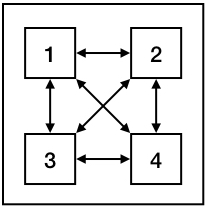
\includegraphics[width=1.0\columnwidth]{local}}
			\caption{Local exchange \label{fig:local_exchange}}
		\end{subfigure}%
		\hspace{1em}%
		\begin{subfigure}{0.53\linewidth}
			\centerline{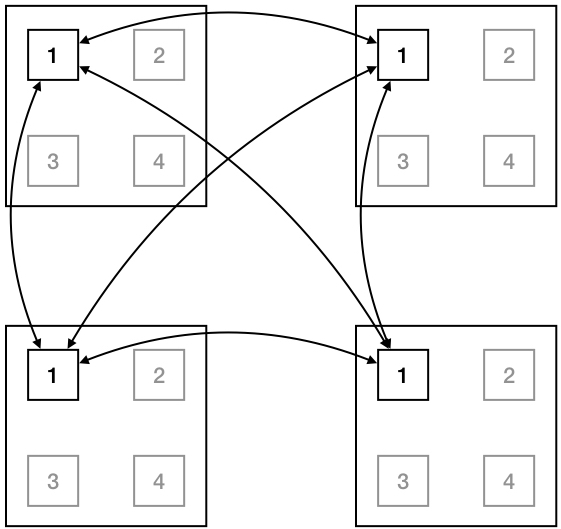
\includegraphics[width=1.0\columnwidth]{remote}}
			\caption{Remote exchange \label{fig:remote_exchange}}
		\end{subfigure}
		\caption{Local and remote exchange diagrams where $N = C = 4$. \label{fig:exchange}}
	\end{center}
\end{figure}


\bigskip
\noindent
\textbf{Node Local}

\noindent
We call the protocol consisting of a local exchange on each node, followed by $C$ remote exchanges that occur in parallel \emph{Node Local}.
%Assume that a message has source $(c_1, n_1)$ and destination $(c_2, n_2)$. 
%In the remote exchange it will be transmit remotely to intermediary $(c_1, n_2)$.
%In the local exchange, it will be transmit locally to its destination. 	
%
%
%The node local strategy consists of a local exchange on each node, followed by $C$ remote exchanges which occur in parallel. 
At the beginning of the local exchange, the process on core $(n,c)$ holds a set of messages to be transmitted.
Each message with destination $(n^\prime, c^\prime)$ is forwarded to $(n, c^\prime)$ in a local exchange, unless $c^\prime = c$, in which case the process holds onto the message.
At the end of this local exchange, each core $(n,c)$ holds messages with addresses of the form $(n^\prime, c)$.
If $n^\prime = n$, then the message has arrived at its destination and is processed. 
Otherwise, it is to be communication in a subsequent remote exchange.
%At the end of this exchange, each message is held by a process matching the destination's core offset.

Once the processor on $(n, c)$ completes its local communication phase, it enters the program context for a remote exchange.
This remote exchange consists of all of the cores with local offset $c$, each of which also hold, or will hold, messages bound for some participant in the exchange.
Once a process has sent all messages routed through it and received all messages sent to it during this ``round'' of communication, it is finished. 
It can safely move on to a different program context, even if others are still working. 

In total, the node local protocol consists of $N$ local exchanges and $C$ remote exchanges, which occur in parallel. 
All messages destined for a particular remote process are accumulated at a single intermediary at each node prior to remote transmission, saving on remote overhead.

While this local aggregate, remote send policy appears adequate for handling point-to-point messages, it is not robust to one-to-many broadcasts.
Such a broadcast results in a total of $NC$ remote messages, which can clearly be improved. 

\bigskip
\noindent
\textbf{Node Remote}

\noindent
Consider the reverse protocol, which we call \emph{Node Remote}.
That is, each process participates in a remote exchange with all cores matching its core offset in the first round of communication, followed by a local exchange at each node in the second. 
For each message held by the process at $(n, c)$ with destination $(n^\prime, c^\prime)$, the process forwards the message to $(n^\prime, c)$ in the remote exchange.
Once all remote exchanges have completed, each message is held on a node matching its destination node offset. 
A local exchange in the second phase ensures that each message arrives at its destination core. 

Whereas the node local protocol accumulates all messages to a particular process in a single intermediary before remote transmission, the node remote protocol instead forwards all messages from a particular process destined for the same \emph{node}, allowing for a similar bundling of messages in shared memory.
If the distribution over sender-receiver pairs is roughly uniform in an application, then the two protocols should exhibit similar performance.
However, node remote performs much better in the presence of a large number of broadcasts. 
In node remote, a broadcast generates only $N-1$ remote messages.
This means that Node Remote uses less bandwidth per broadcast than Node Local, at a gain of $O \left (\frac{1}{C} \right )$.
The broadcasting work is pushed onto the (typically much faster) shared memory local exchanges. 
%However, the opposite relationship is true for many-to-one communications, such as those of a gather or reduce operation.
%We will illustrate these relationships in greater detail in Section~\ref{async:sec:experiments}.

\bigskip
\noindent
\textbf{NLNR}

\noindent
Both the Node Local and Node Remote protocols exhibit some weaknesses depending upon the distribution of message recipients.
Moreover, each round of each protocol results in $O \left (N^2 \right )$ remote messages, as each processor has $N-1$ possible remote communication partners.
These messages are sent along $C$ parallel communication channels, each including $N$ participating processors.
%We have detailed two protocols thus far, each of which depend upon $C$ independent communication channels, each including $N$ participating cores. 
%As we have discussed, different applications might prefer either the message  node local and node remote protocols.
%However, is it possible to retain qualities of both?

The final protocol we discuss in this document improves upon both the messages per round as well as the communication channel size.
The NLNR protocol reduces the number of remote communication channels to the theoretical minimum, while still allowing each node to communicate directly with every other node by eliminating redundancy.
Consider that a message originating at node $n_1$ might be transmitted along any of $C$ different remote channels to node $n_2$ using node local or node remote.
In NLNR, there is only one channel connecting each such pair of nodes. 

\begin{figure}
	\begin{center}
		\begin{subfigure}{0.45\linewidth}
			\centerline{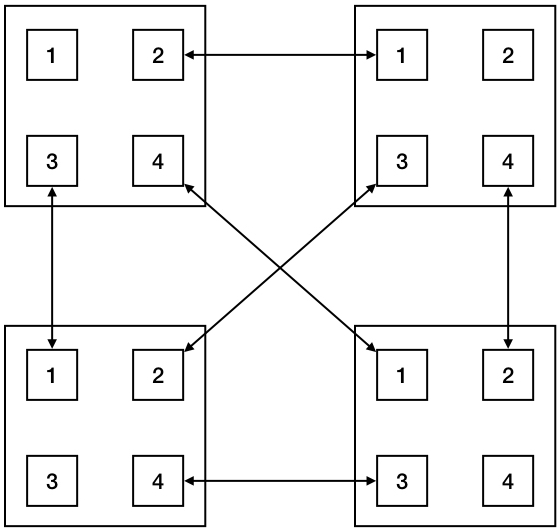
\includegraphics[width=1.0\columnwidth]{intra_layer_nlnr}}
			\caption{Intra-layer communication \label{fig:intra_exchange}}
		\end{subfigure}%
		\hspace{1em}%
		\begin{subfigure}{0.49\linewidth}
			\centerline{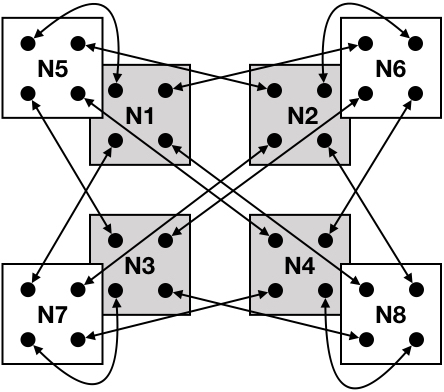
\includegraphics[width=1.0\columnwidth]{inter_layer_nlnr}}
			\caption{Inter-layer communication \label{fig:inter_exchange}}
		\end{subfigure}
		\caption{Intra- and inter-layer exchange diagrams where $N = 8$ and $C = 4$. \label{fig:nlnr}}
	\end{center}
\end{figure}


In order to facilitate this reduction in channels, the protocol need occur in three stages: an initial local exchange, a more complex remote exchange, and a final local exchange.
This more complex remote exchange can be described by taking a clique connecting each node to every other node and assigning to each edge a single core on each incident node.
%It is helpful to separate this clique 
Figure~\ref{fig:nlnr} illustrates an example remote exchange where $N=8$, $C=4$ and $L=2$.

It is helpful to visualize the topology of the remote exchange to explain the whole process. 
We must ensure that each node has an intermediary core responsible for each remote node, so that when viewed as a graph the topology of any subset of nodes and their communication channels forms a clique. 
This constraint leads to a natural ``layering'' of the nodes, where each notional layer consists of $C$ nodes. 
For convenience, in addition to their node offset $n \in [N]$, we assign to each node a \emph{layer offset} $\ell = n \mod C$.
Further, we enforce the rule that $(n,c) \in [N] \times [C]$ is an intermediary for all cores on node $n^\prime$, where $c = n^\prime \mod C$ with corresponding intermediaries $(n^\prime, c^\prime)$ where $c^\prime = n \mod C$. 
Fig.~\ref{fig:intra_layer_nlnr} depicts such a topology for a single layer, whose connections form a clique. 
Note that cores with addresses of the form $(n, c)$ where $c = n \mod C$ do not participate in any communication within a layer. 
These cores only communicate with their corresponding cores in nodes whose layer offsets match their own. 
Fig.~\ref{fig:inter_layer_nlnr} depicts an example inter-layer communication topology  for two layers. 
Intra-layer edges are suppressed for clarity. 
The edges in Fig.~\ref{fig:inter_layer_nlnr} mirror those of Fig.~\ref{fig:intra_layer_nlnr} aside from the addition of the self-offset edges missing from Fig.~\ref{fig:intra_layer_nlnr}.
Note that by adding the edges from Fig.~\ref{fig:intra_layer_nlnr} to both layers, we have a clique.


\begin{figure}[htbp] 
\centerline{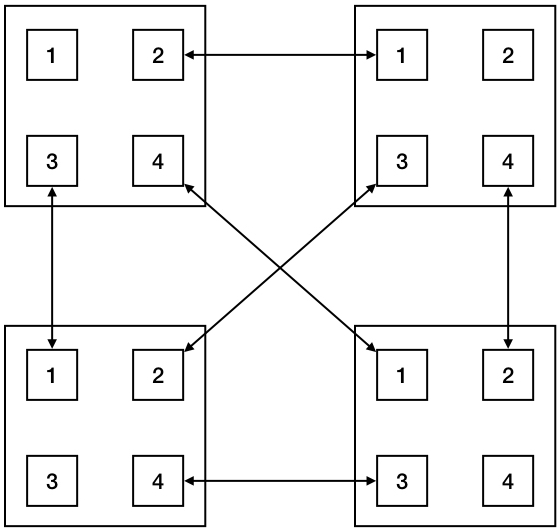
\includegraphics[width=0.6\columnwidth]{intra_layer_nlnr}}
\caption{Example of the remote communication topology within a single layer of 4-core machines in the nlnr protocol.
\label{fig:intra_layer_nlnr}}
\end{figure}

\begin{figure}[htbp] 
\centerline{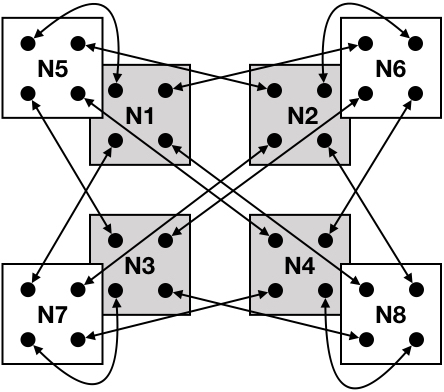
\includegraphics[width=0.6\columnwidth]{inter_layer_nlnr}}
\caption{Example of the remote communication topology between two layers of 4-core machines in the nlnr protocol.
\label{fig:inter_layer_nlnr}}
\end{figure}

In the first local exchange on node $n$, a message from $(n, c)$ with destination $(n^\prime, c^\prime)$ is forwarded to $(n, n^\prime \mod C)$.
In the remote exchange, this message is sent to $(n^\prime, n \mod C)$.
In the final local exchange, the message arrives at $(n^\prime, c^\prime)$.
If any of these intermediate cores are the destination, it is received there and not forwarded. 

If a process needs to broadcast to all other processes, then it sends this message to each of its local neighbors, who forward it along to each of their local partners, who in turn distribute it on each remote node.
Like the node remote protocol, a broadcast over NLNR results in $N-1$ remote messages. 

While point to point messages are transmitted at most twice in node local and node remote, they might be transmitted up to 3 times in NLNR. 
While the local shared memory transmissions are less costly than remote transmissions over a wire, they are still not trivial and so this can result in overhead not seen in the other two protocols. 
However, in exchange we significantly reduce the number of channels over which remote messages traverse.
Recall that node local and node remote each require $C$ communication channels, each of which includes the $N$ cores with matching core offset $c$ for each $c \in [C]$. 
NLNR, however, requires ${C \choose 2} + C$ channels, each including $2\frac{N}{C}$ cores (aside from the self-offset channels, which include $\frac{N}{C}$ cores each).
Such a channel consists of all the address pairs $(n, c)$, $(n^\prime, c^\prime)$ where $c = \ell^\prime = n^\prime \mod C$ and $c^\prime = \ell = n \mod C$ for some $(\ell, \ell^\prime) \in [C]^2$.

%It turns out that this is, in fact, the minimum achievable channel size  given our constraint that each node communications directly with each other node.
It is worth noting that there are many other specific assignments of cores to channels possible. 
We did not find that other assignments exhibited sufficiently different behavior, and so we will forgo a discussion thereof. 

%----------------------------------------------------------------------------------------
\section{Experiments} \label{async:sec:experiments}
%----------------------------------------------------------------------------------------











%----------------------------------------------------------------------------------------
%----------------------------------------------------------------------------------------
\chapter{\algoname{DegreeSketch} with Applications to Neighborhood Approximation and Local Triangle Count Heavy Hitter Estimation}
 \label{chap:DS}
%----------------------------------------------------------------------------------------
%----------------------------------------------------------------------------------------


In this chapter we present \algoname{DegreeSketch}, a semi-streaming distributed sketch datastructure and demonstrate its utility for estimating local triangle count heavy hitters.
\algoname{DegreeSketch} consists of vertex-centric cardinality sketches distributed across a set of processors. 
While other semi-streaming approaches to estimating local triangle counts depend on sampling, \algoname{DegreeSketch} is a persistent queryable data structure.
We discuss the advantages and limitations of this approach, and present empirical results.

%----------------------------------------------------------------------------------------
\section{Introduction and Related Work}
 \label{DS:sec:intro}
%----------------------------------------------------------------------------------------

Counting the number of triangles in graphs is a canonical problem in both the RAM and streaming models.
A ``triangle'' is a trio of co-adjacent vertices, and is the smallest nontrivial community structure.
Consequently, triangles and triangle counting arise often in applications.
Both the global count of triangles and the vertex-local counts, i.e. the number of triangles incident upon each vertex, are key to network analysis and graph theory topics such as cohesiveness \cite{lim2015mascot}, global and local clustering coefficients \cite{tsourakakis2008fast}, and trusses \cite{cohen2008trusses}.
These counts are also directly useful in many applications, such as spam detection \cite{becchetti2010efficient},  community discovery \cite{wang2010triangulation, berry2011tolerating}, and protein interaction analysis \cite{milo2002network}.

Although not traditionally considered a centrality index, one can think of the number of triangles incident upon a vertex as a generalization of its degree centrality. 
To wit, we define the \emph{triangle count centrality} of a vertex $x \in \mathcal{V}$ as
%
\begin{equation}
	\mathcal{C}^{\algoname{Tri}}(x) = |\{yz \in \mathcal{E} \mid xy, zx \in \mathcal{E} \wedge |\{x, y, z\}| = 3\}|.
\end{equation}
%
Similarly, we can consider the triangle count centrality of edges as well, defined similarly as
%
\begin{equation}
	\mathcal{C}^{\algoname{Tri}}(xy) = |\{z \in \mathcal{V} \setminus \{x,y\} \mid yz, zx \in \mathcal{E}\}|.
\end{equation}
%

Although many exact algorithms have been proposed for the triangle counting problem \cite{tsourakakis2008fast, becchetti2010efficient, chu2011triangle, suri2011counting, wolf2017fast}, their time complexity is superlinear in the number of edges, $O(m^{
\frac{3}{2}})$.
Consequently, these analyses are expensive on very large graphs, particularly if they are dense.
While there is a rich literature centered on the exact global and local triangle counting problem, we will not exhaustively recall it in this document.

In order to avoid the dreaded superlinear scaling of exact algorithms, many researchers have turned to approximation.
Several streaming local triangle counting algorithms have been proposed in recent years.
These serial streaming algorithms  maintain a limited number of sampled edges from an edge stream.
Streaming global triangle estimation algorithms have arisen that sample edges with equal probability \cite{tsourakakis2009doulion}, sample edges with probability relative to counted adjacent sampled edges and incident triangles \cite{ahmed2017sampling}, and sample edges along with paths of length two \cite{jha2013space}. 
The first proposed semi-streaming local triangle estimation algorithm relies upon min-wise independent permutations accumulated over a logarthmic number of passes \cite{becchetti2008efficient}. 
More recently, true single-pass algorithms have arisen such as \algoname{Mascot} \cite{lim2015mascot}, which maintains local estimates that are updated whether an observed edge is sampled or not.
Similarly, \algoname{Tri\'est} \cite{stefani2017triest} utilizes reservoir sampling, possibly disposing of sampled edges when a new edge is observed if system memory is saturated.
This affords robustness to dynamic streams, as well as reducing variance.
None of these algorithms perform edge-local triangle counting.

While many distributed global and vertex-local triangle counting algorithms have been proposed, the overwhelming majority store the graph in distributed memory and return exact solutions using \algoname{MapReduce} \cite{suri2011counting} or distributed memory \cite{arifuzzaman2013patric, pearce2017triangle}.
Recently, the study of distributed streaming vertex-local triangle counting was intiated in earnest with the presentation of \algoname{Try-Fly} \cite{shin2018tri}, which maintains parallel instantiations of \algoname{Tri\'est$_{\algoname{Impr}}$}.
A controller node feeds partitions of the graph stream to each of these instances in order to boost estimation accuracy and speed.
\algoname{DiSLR} \cite{shin2018dislr} improves upon \algoname{Try-Fly} by introducing limited redundancy into the graph stream partitions.
Although \algoname{Try-Fly} and \algoname{DiSLR} are the most similar examples in the literature to our approach, we use distinct methods.

Our approach is fundamentally different, depending upon sketching rather than sampling as its core primitive. 
While the sampling approaches produce estimates, we produce a leave-behind queryable data structure similar in interface to \algoname{CountMinSketch}.

%These algorithms depends upon sampling edges from an edge stream in order to assemble a sparse graph, whose triangles are then used to estimate the true local triangle counts.
%The most successful recent algorithm \algoname{Tri\'est} utilizes reservoir sampling to afford dynamic graph streams as well as to affect a reduction in variance.
%Very recent distributed streaming algorithms boost the performance of underlying sampling algorithms such as \algoname{Tri\'est} by utilizing parallel machines operating on partitions of the input graph \cite{shin2018tri, shin2018dislr}.

%----------------------------------------------------------------------------------------
\section{\algoname{DegreeSketch} via Distributed Cardinality Sketches}
 \label{DS:sec:DS}
%----------------------------------------------------------------------------------------

We take a different approach to estimating local triangle counts, relying upon sketches instead of sampling.
We introduce \algoname{DegreeSketch}, a cardinality sketch-based distributed data structure trained on graph streams.
We will first describe \algoname{DegreeSketch} at a high level, describe algorithms that utilize it in Sections~\ref{DS:sec:neighborhoods}, ~\ref{DS:sec:edge_triangles}, and ~\ref{DS:sec:vertex_triangles} and then discuss implementation details using the \algoname{HyperLogLog} cardinality sketch in Section~\ref{DS:sec:HLL}.

\algoname{DegreeSketch} maintains a data structure $\mathcal{D}$ that can be queried for an estimate of a vertex's degree, similar in interface to the celebrated \algoname{CountSketch} \cite{charikar2002finding} and \algoname{CountMinSketch} \cite{cormode2005improved}.
This data structure is organized not unlike the sampling sketch approach to graph sparsification discussed in Section~\ref{sec:spanner}, with sketches summarizing the local information for each $x \in \mathcal{V}$.
For each $x \in \mathcal{V}$ we maintain a cardinality sketch $\mathcal{D}[x]$, which affords the approximation of $\mathbf{d}_x$, the degree of $x$. 
%We obtain estimates of local triangle counts by comparing the sketches of adjacent vertices.

It is known that any data structure that provides relative error guarantees for the cardinality of a multiset with $n$ unique elements requires $O(n)$ space \cite{alon1999space}.
Consequently, investigators have developed many so-called \emph{cardinality sketches} that provide such relative error guarantees while admitting a small probability of failure, such as PCSA \cite{flajolet1985probabilistic}, MinCount \cite{bar2002counting},  LogLog \cite{durand2003loglog}, Multiresolution Bitmap \cite{estan2003bitmap}, HyperLogLog \cite{flajolet2007hyperloglog}, and the space-optimal solution of \cite{kane2010optimal}.
While all these cardinality sketches have a natural union operation that allows one to combine the sketches of two multisets into a sketch of their union, most have no closed intersection operation.

For the purposes of discussion, we will abstract the particulars of cardinality sketches until Section~\ref{DS:sec:HLL}.
We assume that the sketches provide a $\varepsilon$-approximation of the number of unique items in a stream using $\Omega(\varepsilon^{-2})$ space.
We assume that the sketches support an \algoname{Insert} operation to add elements, a \algoname{Merge} operation to combine sketches, an \algoname{Estimate} operation to estimate cardinalities, and an \algoname{EstimateIntersection} operation to estimate intersection cardinalities.
For reasons that will be described in Section~\ref{DS:sec:HLL:intersection}, we do not assume that the \algoname{EstimateIntersection} procedure has the same error and variance properties as the guarantees for \algoname{Estimate}.

We will describe the accumulation of a \algoname{DegreeSketch} instance on a universe of processors $\mathcal{P}$. 
We assume that the undirected graph $\mathcal{G} = (\mathcal{V}, \mathcal{E})$ is given by a stream $\boldsymbol{\sigma}$.
$\boldsymbol{\sigma}$ is further partitioned by some unknown means into $|\mathcal{P}|$ substreams.
We assume that each processor $P \in \mathcal{P}$ has send and receive buffers $\mathcal{S}[P]$ and $\mathcal{R}[P]$, respectively.
We will make no assumptions in the following algorithms how processors handle switching context between processing and sending and receiving communication. 
In our implementations we use the software package \algoname{YGM} described in Chapter~\ref{chap:async}.
We further assume that there is some partitioning of vertices to processors $f : \mathcal{V} \rightarrow \mathcal{P}$. 
We will occasionally abuse notation and use $f(P)$ to describe the set of vertices that map to $P \in \mathcal{P}$.
We make no assumptions about the particulars of $f$, noting that vertex partitionings are a subject of intense academic scrutiny as discussed in Section~\ref{async:sec:intro:partitioning}.

Algorithm~\ref{alg:ds:accumulation} describes the distributed accumulation of a \algoname{DegreeSketch} instance.
In a distributed pass over the partitioned stream, processors use the partition function $f$ to send edges to the cognizant processors for each endpoint. 
These processors each maintain cardinality sketches for their assigned vertices.
When $P \in \mathcal{P}$ receives an edge $xy \in \mathcal{E}$ where $f(x) = P$, it performs $\algoname{Insert}(\mathcal{D}[x], y)$.
Once all processors are done reading and communicating, $\mathcal{D}$ is accumulated.

\begin{algorithm}[htbp] 
\caption{\algoname{DegreeSketch} Accumulation}\label{alg:ds:accumulation}
\begin{flushleft}
        \textbf{Input:} 		$\boldsymbol{\sigma}$ - edge stream divided into $|\mathcal{P}|$ substreams\\
        	\hspace{3.2em}	$\mathcal{P}$ - universe of processors	 \\
%        	\hspace{2.65em}	$\mathcal{D}$ - distributed dictionary mapping $\mathcal{V}$ to cardinality sketches	 \\
        	\hspace{3.2em}	$\mathcal{S}$ - distributed dictionary mapping $\mathcal{P}$ to send queues	 \\
        	\hspace{3.2em}	$\mathcal{R}$ - distributed dictionary mapping $\mathcal{P}$ to receive queues	 \\
        	\hspace{3.2em}	$f$ - function mapping $\mathcal{V} \rightarrow \mathcal{P}$	 \\
        \textbf{Output:} $\mathcal{D}$ - accumulated DegreeSketch
\end{flushleft}
\begin{flushleft}
\begin{algorithmic}[1]
	\Statex \textbf{Send Context} for $P \in \mathcal{P}$:
		\While{$\mathcal{S}[P]$ is not empty}
  			\State $(W, xy) \gets \mathcal{S}[P].\pop$
			\State $\mathcal{R}[W].\push{xy}$
  		\EndWhile
	\Statex \textbf{Receive Context} for $P \in \mathcal{P}$:
		\While{$\mathcal{R}[P]$ is not empty}
  			\State $xy \gets \mathcal{R}[P].\pop$
  			\If {$!\exists \mathcal{D}[x]$} 
				\State $\mathcal{D}[x] \gets \text{empty sketch}$
			\EndIf
	  		\State $\algoname{Insert}(\mathcal{D}[x], y)$
  		\EndWhile
	\Statex \textbf{Accumulation Context} for $P \in \mathcal{P}$:
		\State $\mathcal{D} \gets $ empty $\algoname{DegreeSketch}$ dictionary
		\While{$\sigma_P$ has unread element $uv$}
			\State $U \gets f(u)$
 			\State $\mathcal{S}[P].\push{U, uv}$
			\State $V \gets f(v)$
 			\State $\mathcal{S}[P].\push{V, vu}$
		\EndWhile
		\State \Return $\mathcal{D}$
\end{algorithmic}
\end{flushleft}
\end{algorithm}



\algoname{DegreeSketch} can be implemented with any cardinality sketch that admits some form of union and intersection estimation.
In fact, the algorithms in Sections~\ref{DS:sec:edge_triangles} and ~\ref{DS:sec:vertex_triangles} do not even require a closed merge operation.
In our experiments, we focus on the well-known \algoname{HyperLogLog} or \algoname{HLL} cardinality sketches.
We use \algoname{HLL}s for implementation due to several attractive features:
\begin{enumerate}
	\item Small register size
	\item Simple merge operation
	\item Sparse register representation
	\item Adequate intersection estimator
\end{enumerate}

We introduce \algoname{HLL} and discuss these features in greater detail in Section~\ref{DS:sec:hll}.
FIrst, however, we describe algorithms utilizing \algoname{DegreeSketch} for neighborhood size estimation in Section~\ref{DS:sec:neighborhoods}, recovering edge-local triangle count heavy hitters in Section~\ref{DS:sec:edge_triangles}, and finally recovering vertex-local triangle count heavy hitters in Section~\ref{DS:sec:vertex_triangles}.

%----------------------------------------------------------------------------------------
\section{Neighborhood Size Estimation}
 \label{DS:sec:neighborhoods}
%----------------------------------------------------------------------------------------

Let the neighborhood function $\mathcal{N}_\mathcal{G}(t)$ be defined by 
%
\begin{equation} \label{eq:func:nbhd}
	\mathcal{N}_\mathcal{G}(t) = |\{(x, y) \in \mathcal{V} \times \mathcal{V} | d_\mathcal{G}(x, y) < t\}|.
\end{equation}
%
This function provides data about how fast the ``average ball'' around each $x \in \mathcal{V}$ expands, permitting the estimation of $G$'s properties such as the effective diameter \cite{palmer2002anf}.
For $t \in \mathbf{N}$, let $\mathcal{N}_\mathcal{G}^t(x)$ be the \emph{local} neighborhood function defined as 
%
\begin{equation} \label{eq:func:nbhd:local}
	\mathcal{N}_\mathcal{G}^t(x) = |\{y \in \mathcal{V} | d_\mathcal{G}(x, y) < t\}|.
\end{equation}
%
We will drop the subscripts where they are clear.
In particular, we have that 
%
\begin{equation} \label{eq:func:nbhd:sum}
	\mathcal{N}(t) = \sum_{x \in \mathcal{V}} \mathcal{N}^t(x).
\end{equation}
%
The \algoname{ANF} \cite{palmer2002anf} and \algoname{HyperANF} \cite{boldi2011hyperanf} algorithms estimate $\mathcal{N}^t(x)$ for each $x \in \mathcal{V}$ using Flajolet-Martin and \algoname{HyperLogLog} cardinality sketches, respectively, and produce estimates of $\mathcal{N}(t)$ of the form Eq.~\eqref{eq:func:nbhd:sum}.

Let $\mathcal{D}$ be an instance of \algoname{DegreeSketch} as described, so that for $x \in \mathcal{V}$, $\mathcal{D}[x]$ is a cardinality sketch of the adjacency set of $x$.
Assume that there is an approximate union operator $\widetilde{\cup}$.
If we have $A_{:,x}$, then we can compute an estimate of $\mathcal{N}^2(x)$ by computing 
%
\begin{equation} \label{eq:estimate:nbhd}
	\widetilde{\mathcal{N}}^2(x) 
	= \widetilde{\bigcup}_{y: A_{y,x} \neq 0} \mathcal{D}[y].
\end{equation}
%

Higher-order merge operations described by Eq.~(\ref{eq:estimate:nbhd}) form the core of the \algoname{ANF} \cite{palmer2002anf} and \algoname{HyperANF} \cite{boldi2011hyperanf} algorithms.
We will restrict further analysis to \algoname{HyperANF}.
\algoname{HyperANF} uses HyperLogLog sketches similar to \algoname{DegreeSketch} to estimate the $t$-hop neighborhood sizes of all vertices by way of a iterative sketch merging procedure, which is useful for applications such as edge prediction in social networks \cite{gupta2013wtf} and probabilistic distance calculations \cite{boldi2011hyperanf, myers2014information}.
However, \algoname{HyperANF} also requires storing the whole graph in memory in addition to the \algoname{DegreeSketch} data structure, and is optimized for shared but not distributed memory. 
It also does not take advantage of recent advances in HyperLogLog joint estimation that permit reasonable estimation of sketch intersections as well as unions.


\begin{algorithm}[htbp] 
\caption{\algoname{DegreeSketch} Neighborhood Approximation}\label{alg:ds:anf}
\begin{flushleft}
        \textbf{Input:} 		$\boldsymbol{\sigma}$ - edge stream divided into $|\mathcal{P}|$ substreams\\
        	\hspace{3.2em}	$\mathcal{P}$ - universe of processors	 \\
        	\hspace{3.2em}	$\mathcal{D}^1$ - accumulated \algoname{DegreeSketch} 	 \\
        	\hspace{3.2em}	$\mathcal{S}$ - distributed dictionary mapping $\mathcal{P}$ to send queues	 \\
        	\hspace{3.2em}	$\mathcal{R}$ - distributed dictionary mapping $\mathcal{P}$ to receive queues	 \\
        	\hspace{3.2em}	$f$ - function mapping $\mathcal{V} \rightarrow \mathcal{P}$	 \\
        \textbf{Output:} $\mathcal{N}(t)$ for all $t > 1$
\end{flushleft}
\begin{flushleft}
\begin{algorithmic}[1]
	\Statex \textbf{Send Context} for $P \in \mathcal{P}$:
		\While{$\mathcal{S}[P]$ is not empty}
			\If {next message is an \algoname{Edge}}
	  			\State $(W, xy, t) \gets \mathcal{S}[P].\pop$
				\State $\mathcal{R}[W].\push{\algoname{Edge}, xy, t}$
			\ElsIf{next message is a \algoname{Sketch}}
				\State $(W, \mathcal{D}[x], y, t) \gets \mathcal{S}[P].pop()$
				\State $\mathcal{R}[W].\push{\algoname{Sketch}, y, t}$
			\EndIf
  		\EndWhile
	\Statex \textbf{Receive Context} for $P \in \mathcal{P}$:
		\While{$\mathcal{R}[P]$ is not empty}
			\If {next message is an \algoname{Edge}}
	  			\State $(xy, t) \gets \mathcal{R}[P].\pop$
				\State $Y \gets f(y)$
				\State $\mathcal{S}[P].\push{\algoname{Sketch}, (Y, \mathcal{D}^{t-1}[x], y, t)}$
			\ElsIf{next message is a \algoname{Sketch}}
				\State $(\mathcal{D}^{t-1}[x], y, t) \gets \mathcal{R}[P].\pop$
				\State $\mathcal{D}^t[y] \gets \algoname{Merge}(\mathcal{D}^t[y], \mathcal{D}^{t-1}[x])$
			\EndIf
  		\EndWhile
	\Statex \textbf{Execution Context} for $P \in \mathcal{P}$:
		\State $t \gets 1$
		\State $\mathcal{N}(0) \gets |\mathcal{V}|$
		\State $\mathcal{N}_P(1) \gets \sum\limits_{x \in f(P)} \algoname{Estimate}(\mathcal{D}^1[x])$ \label{alg:ds:anf:line:sum1}
		\State $\mathcal{N}(1) \gets \algoname{Reduce}(\algoname{Sum}, \mathcal{N}_P(1))$
		\While{$\mathcal{N}(t) \neq \mathcal{N}(t-1)$}
			\State $t \gets t + 1$
			\State $\mathcal{D}^t \gets $ empty \algoname{DegreeSketch} dictionary
			\While{$\sigma_P$ has unread element $uv$}
				\State $U \gets f(u)$
	 			\State $\mathcal{S}[P].\push{\algoname{Edge}, (U, uv, t)}$
				\State $V \gets f(v)$
 				\State $\mathcal{S}[P].\push{\algoname{Edge}, (V, vu, t)}$
			\EndWhile
			\State $\mathcal{N}_P(t) \gets \sum\limits_{x \in f(P)} \algoname{Estimate}(\mathcal{D}^t[x])$ \label{alg:ds:anf:line:sum2}
			\State $\mathcal{N}(t) \gets \algoname{Reduce}(\algoname{Sum}, \mathcal{N}_P(t))$
			\State replace $\mathcal{D}^{t-1}$ with $\mathcal{D}^t$
		\EndWhile
\end{algorithmic}
\end{flushleft}
\end{algorithm}

Algorithm~\ref{alg:ds:anf} uses ~\algoname{DegreeSketch} to recreate the behavior of \algoname{HyperANF}.
After accumulating $\mathcal{D}^1$, an instance of \algoname{DegreeSketch}, the algorithm takes a number of additional passes over $\boldsymbol{\sigma}$. 
For $t$ starting at 2, we accumulate 
%
\begin{equation} \label{eq:nextlayer}
\mathcal{D}^t[x] = \widetilde{\bigcup}_{y: xy \in \mathcal{E}} \mathcal{D}^{t-1}[y]
\end{equation}
%
by way of a message-passing scheme similar to Algorithm~\ref{alg:ds:accumulation}.
When $P \in \mathcal{P}$ receives an edge $xy \in \mathcal{E}$ where $f(x) = P$, it forwards $\mathcal{D}^{t-1}[x]$ to $Y = f(y)$.
When $Y$ receives this sketch, it merges it into its next layer local sketch for $y$, $\mathcal{D}^t[y]$, computing Eq.~\eqref{eq:nextlayer} once all messages are processed.
By construction, we have that
%
\begin{equation} \label{eq:nextlayer:full}
\mathcal{D}^t[x] = \widetilde{\bigcup}_{y: d(x,y) = s < t-1} \mathcal{D}^{s}[y].
\end{equation}
%
Ergo, the set of elements inserted into $\mathcal{D}^t[x]$ consists of all $y \in \mathcal{V}$ such that $d(x,y) < t$, which is to say that $\mathcal{D}^t[x]$ directly approximates $\mathcal{N}^t(x)$ (Eq.~\eqref{eq:func:nbhd:local}). 
Ergo, the summations over all sketches in lines \ref{alg:ds:anf:line:sum1} and \ref{alg:ds:anf:line:sum2} of Algorithm~\ref{alg:ds:anf} estimate $\mathcal{N}(t)$ in the same way as does the equivalent procedure in \algoname{HyperANF}.
Note that these summations are performed as distributed \algoname{Reduce} operations.
In addition to returning estimates of the neighborhood function, this procedure can be used to return estimates of the local $t$-degree neighborhoods of vertices, which have their own uses.
Furthermore, as the actual estimates produced by Algorithm~\ref{alg:ds:anf} as the same as those produced by \algoname{HyperANF}, all of the statistical results of \cite{boldi2011hyperanf} apply.
We reproduce the following theorem, although the other theorems and corollaries of \cite{boldi2011hyperanf} also apply. 

\begin{theorem}
The output $\widetilde{\mathcal{N}}(t)$ of Algorithm~\ref{alg:ds:anf} at the $t$-th iteration satisfies 
%
\begin{equation*}
	\frac{\E \left [ \widetilde{\mathcal{N}}(t) \right ]}{\mathcal{N}(t)} = 1 + \delta_1(n) + o(1) \textnormal{ for $n \rightarrow \infty$,}
\end{equation*}
%
where $\delta_1(n)$ is the same as in \cite{flajolet2007hyperloglog} Theorem 1, and $|\delta_1(x)| < 5 \cdot 10^{-5}$ when $r \geq 16$.

Furthermore, let $\widetilde{\mathcal{N}}^t(\cdot)$ be the local output of Algorithm~\ref{alg:ds:anf} (i.e. $\widetilde{\mathcal{N}}^t(x) = \algoname{Estimate}(\mathcal{D}^t[x]$).
Each of these estimates shares the standard deviation $\eta_r$ given by \cite{flajolet2007hyperloglog}, which is also shared by $\widetilde{N}(t)$. 
That is, 
%
\begin{equation*}
	\frac{\sqrt{\Var \left [ \widetilde{\mathcal{N}}(t)\right ]}}{\mathcal{N}(t)} \leq \eta_r.
\end{equation*}
%
%Implementing Algorithm~\ref{alg:ds:anf} with \algoname{HyperLogLog} sketches requires $\widetilde{O}(m)$ time and bits of communication, and only $O(n ( \varepsilon^{-1}\log\log n + \log n))$ space.
\end{theorem}

\begin{proof}
The proof of the first two claims is the same as the proof of Theorem 1 in \cite{boldi2011hyperanf}, so we will not reproduce it here.
\end{proof}

%Rather than inserting received edges into sketches, however, processors forward


Unlike \algoname{HyperANF}, Algorithm~\ref{alg:ds:anf} is distributed and streaming, and does not require the storage of $\mathcal{G}$ in memory. 
However, it is also not optimized to take advantage of shared memory task decomposition or multicore optimizations using \emph{broadword programming} like \algoname{HyperANF}.
It is possible to design an algorithm that supports these features, but we do not produce it here as it would be out of scope. 
We will instead describe it at a high level.
Rather than each core on each node operating independently, each node would act as an instance of \algoname{HyperANF} on a partition of the graph, communicating sketches to other nodes as needed like Algorithm~\ref{alg:ds:anf}.
Merges and estimates would make use of all of the shared memory cores, utilizing the broadword programming approach given in Section 3 of \cite{boldi2011hyperanf}.

%----------------------------------------------------------------------------------------
\section{Edge-Local Triangle Count Heavy Hitters}
 \label{DS:sec:edge_triangles}
%----------------------------------------------------------------------------------------

In addition to estimating local neighborhood sizes, \algoname{DegreeSketch} affords an analysis of local triangle counts using intersection estimation. 
Furthermore, while sampling-based streaming algorithms are limited to vertex-local triangle counts, \algoname{DegreeSketch} affords the analysis of edge-local triangle counts. 
Edge-local triangle counts, i.e. the number of triangles in which each edge participate, can be thought of as a generalization of vertex-local triangle counts. 
Given the edge-local triangle counts for each edge incident upon a vertex, we can easily compute its vertex-local triangle count.
Specifically,
%
\begin{equation} \label{eq:sum_of_edge_tris}
	\mathcal{C}^\algoname{Tri}(x) 
	= \frac{1}{2}\sum\limits_{xy \in \mathcal{E}} \mathcal{C}^\algoname{Tri}(xy)
\end{equation}
%
The reverse is not true. 

Edge-local triangle counts have understandably not received much attention in the streaming literature, considering that even enumerating them requires $\Omega(m)$ space. 
Given an accumulated \algoname{DegreeSketch} $\mathcal{D}$ and intersection operator $\widetilde{\cap}$, for $xy \in \mathcal{E}$ we can estimate $\mathcal{C}^{\algoname{Tri}}(xy)$ using 
%
\begin{equation} \label{eq:tri:edge}
	\widetilde{\mathcal{C}}^{\algoname{Tri}}(xy) 
	= \mathcal{D}[x] \widetilde{\cap} \mathcal{D}[y].
\end{equation}
%
This procedure is similar to the well-known intersection method for local triangle counting. 
Indeed, we can estimate the total number of triangles $\mathcal{T}$ in the graph by computing
%
\begin{equation} \label{eq:tri:total}
	\widetilde{\mathcal{T}} 
	= \frac{1}{3} \sum\limits_{xy \in \mathcal{E}} 	\widetilde{\mathcal{C}}^{\algoname{Tri}}(xy) 
	= \frac{1}{3} \sum\limits_{xy \in \mathcal{E}} \mathcal{D}[x] \widetilde{\cap} \mathcal{D}[y].
\end{equation}
%


Unfortunately, while most cardinality sketches have a native and closed $\widetilde{\cup}$ operation, they all lack a satisfactory intersection operation.
This is not surprising, as sketches are in effect lossy compressions. 
Indeed, it is known that the detection of a trivial intersection is impossible in sublinear memory. 
Hence, we must instead make use of unsatisfactory intersection operations in practice, which has been a focus of recent research \cite{ting2016towards, cohen2017minimal, ertl2017new}.
We will discuss these in more detail in Section~\ref{DS:sec:HLL:intersection}, and their shortcomings in Section~\ref{DS:sec:intersections}.
For our purposes, we will suppose that $\widetilde{\cap}$ is reliable only where intersections are large.
Consequently, we will attempt only to recovery the heavy hitters of $\mathcal{C}^{Tri}$. 

Algorithm~\ref{alg:ds:chassis} provides a chassis for Algorithms~\ref{alg:ds:edge_local}  and ~\ref{alg:ds:vertex_local}, which differ only in their communication behavior. 
In Algorithm~\ref{alg:ds:chassis}, all processors read over their edge streams and forward edges to one of their endpoints, similar to the behavior in the \textbf{Accumulation Context} of Algorithm~\ref{alg:ds:anf}.
They also initialize a counter $\widetilde{\mathcal{T}}$ and a min heap with a maximum size of $k$, $\widetilde{\mathcal{H}}_k$. 
These values are modified in the send and receive contexts of Algorithms~\ref{alg:ds:edge_local}  and ~\ref{alg:ds:vertex_local}.

\begin{algorithm}[htbp] 
\caption{Local Triangle Count Heavy Hitters Chassis}\label{alg:ds:chassis}
\begin{flushleft}
        \textbf{Input:} 		$\boldsymbol{\sigma}$ - edge stream divided into $|\mathcal{P}|$ substreams\\
        	\hspace{3.2em}	$k$ - integral heavy hitter count	 \\
        	\hspace{3.2em}	$\mathcal{P}$ - universe of processors	 \\
        	\hspace{3.2em}	$\mathcal{D}$ - accumulated \algoname{DegreeSketch} 	 \\
        	\hspace{3.2em}	$\mathcal{S}$ - distributed dictionary mapping $\mathcal{P}$ to send queues	 \\
        	\hspace{3.2em}	$\mathcal{R}$ - distributed dictionary mapping $\mathcal{P}$ to receive queues	 \\
        	\hspace{3.2em}	$f$ - function mapping $\mathcal{V} \rightarrow \mathcal{P}$	 \\
%        \textbf{Output:} $\widetilde{\mathcal{T}}$, $\widetilde{\mathcal{H}}_k$
\end{flushleft}
\begin{flushleft}
\begin{algorithmic}[1]
	\Statex \textbf{Accumulation Context} for $P \in \mathcal{P}$:
		\State $\widetilde{\mathcal{H}}_k \gets $ empty $k$-heap
		\State $\widetilde{\mathcal{T}} \gets 0$
		\While{$\sigma_P$ has unread element $uv$}
			\State $U \gets f(u)$
 			\State $\mathcal{S}[P].\push{\algoname{Edge}, (U, uv)}$
%			\State $V \gets f(v)$
%			\State $\mathcal{S}[P].\push{\algoname{Edge}, (V, vu)}$
		\EndWhile
		\State \algoname{Reduce}  $\widetilde{\mathcal{T}}$
		\State $\widetilde{\mathcal{T}} \gets \frac{1}{3} \widetilde{\mathcal{T}}$
\end{algorithmic}
\end{flushleft}
\end{algorithm}


Algorithm~\ref{alg:ds:edge_local} issues a chain of messages for each read edge, not unlike the procedure in Algorithm~\ref{alg:ds:anf}.
$P$ reads $uv$, and issues a message of type \algoname{Edge} containing $uv$ to $U = f(u)$.
Upon receipt, $U$ issues a message of type \algoname{Sketch} containing $(\mathcal{D}[u], uv)$ to $V = f(v)$.
When $V$ receives this message, it computes $\widetilde{\mathcal{C}}^\algoname{Tri}(uv)$ via Eq.~\eqref{eq:tri:edge} and updates $\widetilde{\mathcal{T}}$ and $\widetilde{\mathcal{H}}_k$. 
Once computation is complete and all receive queues are flushed, the algorithm computes a global \algoname{Reduce} sum to find $\widetilde{\mathcal{T}}$ and similarly finds the global top $k$ estimates via a reduce on $\widetilde{\mathcal{H}}_k$. 
The algorithm returns $\widetilde{\mathcal{T}}/3$ (each triangle is counted 3 times) and $\widetilde{\mathcal{H}}_k$.


\begin{algorithm}[htbp] 
\caption{\algoname{DegreeSketch} Edge-Local Triangle Count Heavy Hitters}\label{alg:ds:edge_local}
\begin{flushleft}
%        \textbf{Input:} 		$\boldsymbol{\sigma}$ - edge stream divided into $|\mathcal{P}|$ substreams\\
%        	\hspace{2.65em}	$k$ - integral heavy hitter count	 \\
%        	\hspace{2.65em}	$\mathcal{P}$ - universe of processors	 \\
%        	\hspace{2.65em}	$\mathcal{D}$ - accumulated \algoname{DegreeSketch} 	 \\
%        	\hspace{2.65em}	$\mathcal{S}$ - distributed dictionary mapping $\mathcal{P}$ to send queues	 \\
%        	\hspace{2.65em}	$\mathcal{R}$ - distributed dictionary mapping $\mathcal{P}$ to receive queues	 \\
%        	\hspace{2.65em}	$f$ - function mapping $\mathcal{V} \rightarrow \mathcal{P}$	 \\
        \textbf{Output:} $\widetilde{\mathcal{T}}$, $\widetilde{\mathcal{C}}^{\algoname{Tri}}(xy)$ for top $k$ edges $xy$
\end{flushleft}
\begin{flushleft}
\begin{algorithmic}[1]
%	\Statex \textbf{Accumulation Context} for $P \in \mathcal{P}$:
%		\State $\widetilde{\mathcal{H}}_k \gets $ empty $k$-heap
%		\State $\widetilde{\mathcal{T}} \gets 0$
%		\While{$\sigma_P$ has unread element $uv$}
%			\State $U \gets f(u)$
% 			\State $\mathcal{S}[P].\push{\algoname{Edge}, (U, uv)}$
%%			\State $V \gets f(v)$
%%			\State $\mathcal{S}[P].\push{\algoname{Edge}, (V, vu)}$
%		\EndWhile
%		\State \algoname{Reduce} $\mathcal{H}$ and $\widetilde{\mathcal{T}}$
%		\State $\widetilde{\mathcal{T}} \gets \frac{1}{3} \widetilde{\mathcal{T}}$
	\Statex \textbf{Send Context} for $P \in \mathcal{P}$:
		\While{$\mathcal{S}[P]$ is not empty}
			\If {next message is an \algoname{Edge}}
	  			\State $(W, xy) \gets \mathcal{S}[P].\pop$
				\State $\mathcal{R}[W].\push{\algoname{Edge}, xy}$
			\ElsIf{next message is a \algoname{Sketch}}
				\State $(W, \mathcal{D}[x], y) \gets \mathcal{S}[P].pop()$
				\State $\mathcal{R}[W].\push{\algoname{Sketch}, xy}$
			\EndIf
  		\EndWhile
	\Statex \textbf{Receive Context} for $P \in \mathcal{P}$:
		\While{$\mathcal{R}[P]$ is not empty}
			\If {next message is an \algoname{Edge}}
	  			\State $xy \gets \mathcal{R}[P].\pop$
				\State $Y \gets f(y)$
				\State $\mathcal{S}[P].\push{\algoname{Sketch}, (Y, \mathcal{D}[x], xy)}$
			\ElsIf{next message is a \algoname{Sketch}}
				\State $(\mathcal{D}[x], xy) \gets \mathcal{R}[P].\pop$
				\State $\widetilde{\mathcal{C}}^\algoname{Tri}(xy) \gets \algoname{EstimateIntersection}(\mathcal{D}[y], \mathcal{D}[x])$
				\State $\widetilde{\mathcal{T}} \gets \widetilde{\mathcal{T}} + \widetilde{\mathcal{C}}^\algoname{Tri}(xy)$
				\If{$\widetilde{\mathcal{C}}^\algoname{Tri}(xy) > \min \mathcal{H}_k$}
					\State insert $\left ( xy, \widetilde{\mathcal{C}}^\algoname{Tri}(xy) \right )$ into $\mathcal{H}_k$
					\If {$|\mathcal{H}_k| > k$}
						\State remove $\min \mathcal{H}_k$
					\EndIf
				\EndIf
			\EndIf
  		\EndWhile
	\Statex \textbf{Execution} for $P \in \mathcal{P}$:
		\State Run Algorithm~\ref{alg:ds:chassis} using these communication contexts
		\State \algoname{Reduce} $\widetilde{\mathcal{H}}_k$
		\State \Return $\widetilde{\mathcal{T}}, \widetilde{\mathcal{H}}_k$
\end{algorithmic}
\end{flushleft}
\end{algorithm}

Algorithm~\ref{alg:ds:edge_local} addresses edge--local triangle count heavy hitter recovery using memory sublinear in the size of $\mathcal{G}$. 
It requires $\widetilde{O}(\varepsilon^{-2}m)$ time and communication, given our assumptions, and a total of $O(\varepsilon^{-2} |\mathcal{V}| \log\log |\mathcal{V}| + \log |\mathcal{V}|)$ space, where DegreeSketch is implemented using $\algoname{HyperLogLog}$ sketches with accuracy parameter  $\varepsilon$. 
Unfortunately, we are unable to provide an analytic bound on the error of this algorithm, due to the nature of sublinear intersection estimation. 
We will explore this problem in Section~\ref{DS:sec:intersections} and provide experimental analysis of Algorithm~\ref{DS:sec:experiments}.

%----------------------------------------------------------------------------------------
\section{Vertex-Local Triangle Count Heavy Hitters}
 \label{DS:sec:vertex_triangles}
%----------------------------------------------------------------------------------------

Given access to a trained \algoname{DegreeSketch} $\mathcal{D}$ and $A_{:,x}$, we can compute an estimate of $\mathcal{C}^{\algoname{Tri}}(x)$ using
%
\begin{equation} \label{eq:tri:vertex}
	\widetilde{\mathcal{C}}^{\algoname{Tri}}(x) 
	= \frac{1}{2} \sum_{y: A_{y,x} \neq 0} \widetilde{\mathcal{C}}^{\algoname{Tri}}(xy)  
	= \frac{1}{2} \sum_{y: A_{y,x} \neq 0} \mathcal{D}[x] \widetilde{\cap} \mathcal{D}[y].
\end{equation}
%

While we are not faced with the space constraint present in Section~\ref{DS:sec:edge_triangles} when contending with simply writing down vertex-local triangle counts, we instead must contend with the dreaded small intersection problem discussed in Section \ref{DS:sec:intersections}.
Consequently, we limit our scope to the recovery of vertex-local triangle count heavy hitters.

Algorithm~\ref{alg:ds:vertex_local} performs vertex-local triangle count estimation in a manner similar to Algorithm~\ref{alg:ds:edge_local} with some additional steps. 
We maintain $\widetilde{\mathcal{C}}^\algoname{Tri}(x)$ for each $x \in \mathcal{V}$, which are of course distributed so that $X = f(x)$ computes $\widetilde{\mathcal{C}}^\algoname{Tri}(x)$. 
It performs similar work for $xy \in \mathcal{E}$ up to the point processor $Y = f(y)$ estimates $\widetilde{\mathcal{C}}^\algoname{Tri}(xy)$. 
Instead of inserting this estimate into a local max heap, we add it to $\widetilde{\mathcal{C}}^\algoname{Tri}(y)$, and forward $(\widetilde{\mathcal{C}}^\algoname{Tri}(xy), x)$ to $X = f(x)$ so that it can add it to $\widetilde{\mathcal{C}}^\algoname{Tri}(x)$.
This message has the \algoname{Est} type, to distinguish it from \algoname{Edge} and \algoname{Sketch} messages.


\begin{algorithm}[htbp] 
\caption{\algoname{DegreeSketch} Vertex-Local Triangle Count Heavy Hitters}\label{alg:ds:vertex_local}
\begin{flushleft}
%        \textbf{Input:} 		$\boldsymbol{\sigma}$ - edge stream divided into $|\mathcal{P}|$ substreams\\
%        	\hspace{2.65em}	$k$ - integral heavy hitter count	 \\
%        	\hspace{2.65em}	$\mathcal{P}$ - universe of processors	 \\
%        	\hspace{2.65em}	$\mathcal{D}$ - accumulated \algoname{DegreeSketch} 	 \\
%        	\hspace{2.65em}	$\mathcal{S}$ - distributed dictionary mapping $\mathcal{P}$ to send queues	 \\
%        	\hspace{2.65em}	$\mathcal{R}$ - distributed dictionary mapping $\mathcal{P}$ to receive queues	 \\
%        	\hspace{2.65em}	$f$ - function mapping $\mathcal{V} \rightarrow \mathcal{P}$	 \\
        \textbf{Output:} $\widetilde{\mathcal{T}}$, $\widetilde{\mathcal{C}}^{\algoname{Tri}}(x)$ for top $k$ vertices $x$
\end{flushleft}
\begin{flushleft}
\begin{algorithmic}[1]
%	\Statex \textbf{Accumulation Context} for $P \in \mathcal{P}$:
%		\State $\widetilde{\mathcal{H}}_k \gets $ empty $k$-heap
%		\State $\widetilde{\mathcal{T}} \gets 0$
%		\While{$\sigma_P$ has unread element $uv$}
%			\State $U \gets f(u)$
% 			\State $\mathcal{S}[P].\push{\algoname{Edge}, (U, uv)}$
%%			\State $V \gets f(v)$
%%			\State $\mathcal{S}[P].\push{\algoname{Edge}, (V, vu)}$
%		\EndWhile
%		\State \algoname{Reduce} $\mathcal{H}$ and $\widetilde{\mathcal{T}}$
%		\State $\widetilde{\mathcal{T}} \gets \frac{1}{3} \widetilde{\mathcal{T}}$
	\Statex \textbf{Send Context} for $P \in \mathcal{P}$:
		\While{$\mathcal{S}[P]$ is not empty}
			\If {next message is an \algoname{Edge}}
	  			\State $(W, xy) \gets \mathcal{S}[P].\pop$
				\State $\mathcal{R}[W].\push{\algoname{Edge}, xy}$
			\ElsIf{next message is a \algoname{Sketch}}
				\State $(W, \mathcal{D}[x], xy) \gets \mathcal{S}[P].pop()$
				\State $\mathcal{R}[W].\push{\algoname{Sketch}, xy}$
			\ElsIf{next message is an \algoname{Est}}
				\State $(Y, \widetilde{\mathcal{C}}^\algoname{Tri}(xy), y) \gets \mathcal{S}[P].pop()$
				\State $\mathcal{R}[T].\push{\algoname{Est}, (\widetilde{\mathcal{C}}^\algoname{Tri}(xy), y)}$
			\EndIf
  		\EndWhile
	\Statex \textbf{Receive Context} for $P \in \mathcal{P}$:
		\While{$\mathcal{R}[P]$ is not empty}
			\If {next message is an \algoname{Edge}}
	  			\State $xy \gets \mathcal{R}[P].\pop$
				\State $Y \gets f(y)$
				\State $\mathcal{S}[P].\push{\algoname{Sketch}, (Y, \mathcal{D}[x], xy)}$
			\ElsIf{next message is a \algoname{Sketch}}
				\State $(\mathcal{D}[x], xy) \gets \mathcal{R}[P].\pop$
				\State $Y \gets f(y)$
				\State $\widetilde{\mathcal{C}}^\algoname{Tri}(xy) \gets \algoname{EstimateIntersection}(\mathcal{D}[y], \mathcal{D}[x])$
				\State $\widetilde{\mathcal{C}}^\algoname{Tri}(x) \gets \widetilde{\mathcal{C}}^\algoname{Tri}(x) + \widetilde{\mathcal{C}}^\algoname{Tri}(xy)$
				\State $\widetilde{\mathcal{T}} \gets \widetilde{\mathcal{T}} + \widetilde{\mathcal{C}}^\algoname{Tri}(xy)$
				\State $\mathcal{S}[P].\push{Y, (\widetilde{\mathcal{C}}^\algoname{Tri}(xy), y)}$
			\ElsIf{next message is an \algoname{Est}}
				\State $(\widetilde{\mathcal{C}}^\algoname{Tri}(xy), y) \gets \mathcal{R}[P]$
				\State $\widetilde{\mathcal{C}}^\algoname{Tri}(y) \gets \widetilde{\mathcal{C}}^\algoname{Tri}(y) + \widetilde{\mathcal{C}}^\algoname{Tri}(xy)$
			\EndIf
  		\EndWhile
	\Statex \textbf{Execution} for $P \in \mathcal{P}$:
		\State $\widetilde{\mathcal{C}}^\algoname{Tri}(x) \gets 0$ for each $x \in f(P)$
		\State Run Algorithm~\ref{alg:ds:chassis} using these communication contexts
			\For {$x \in f(P)$}
				\If {$\widetilde{\mathcal{C}}^\algoname{Tri}(x) > \min \widetilde{\mathcal{H}}_k$}
					\State insert $\left ( x, \widetilde{\mathcal{C}}^\algoname{Tri}(x) \right )$ into $\widetilde{\mathcal{H}}_k$
					\If {$|\widetilde{\mathcal{H}}_k| > k$}
						\State remove $\min \widetilde{\mathcal{H}}_k$
					\EndIf
				\EndIf
			\EndFor
		\State \algoname{Reduce} $\widetilde{\mathcal{H}}_k$
		\State \Return $\widetilde{\mathcal{T}}, \widetilde{\mathcal{H}}_k$
\end{algorithmic}
\end{flushleft}
\end{algorithm}


Algorithm~\ref{alg:ds:vertex_local} addresses vertex--local triangle count heavy hitter recovery using the same asymptotic computation, memory and communication costs as Algorithm~\ref{alg:ds:edge_local}.
Unfortunately, we are similarly unable to provide an a priori analytic bound on the error of this algorithm. 
We do, however, have the following theorem using the subadditivity of the standard deviation (i.e. If $A$ and $B$ have finite variance, $\sqrt{\Var \left [ A + B\right ]} \leq \sqrt{\Var \left [ A\right ]} + \sqrt{\Var \left [ B\right ]}$). 

\begin{theorem} \label{thm:vertex_local:variance}
	Let $\widetilde{\mathcal{C}}^\algoname{Tri}(x)$ be the estimated output of Algorithm~\ref{alg:ds:vertex_local} for $x \in \mathcal{V}$, and that $\widetilde{\mathcal{C}}^\algoname{Tri}(xy)$ is the estimated edge triangle count for each $xy \in \mathcal{E}$.
	Assume further that for each $xy$, we know a standard deviation bound $\eta_{xy}$ so that
	\begin{equation} \label{thm:vertex_local:variance:bound}
		\frac{\sqrt{\Var \left [ \widetilde{\mathcal{C}}^\algoname{Tri}(xy) \right ] }}{\mathcal{C}^\algoname{Tri}(xy)} \leq \eta_{xy}.
	\end{equation}
	Furhermore, let $\eta_{*} = \max_{xy \in \mathcal{E}} \eta_{xy}$.
	Then, $\widetilde{\mathcal{C}}^\algoname{Tri}(x)$ has at most twice this maximum standard deviation.
	That is,
	\begin{equation*}
		\frac{\sqrt{\Var \left [ \widetilde{\mathcal{C}}^\algoname{Tri}(x) \right ] }}{\mathcal{C}^\algoname{Tri}(x)} \leq 2\eta_{*}.
	\end{equation*}
\end{theorem}

\begin{proof}
\begin{align*}
	\frac{\sqrt{\Var \left [ \widetilde{\mathcal{C}}^\algoname{Tri}(x) \right ] }}{\mathcal{C}^\algoname{Tri}(x)}
	&=
	\frac{\sqrt{\Var \left [ \sum\limits_{xy \in \mathcal{E}} \widetilde{\mathcal{C}}^\algoname{Tri}(xy) \right ] }}{\mathcal{C}^\algoname{Tri}(x)}
	& \\
	%&>
	%\sum_{z \in \mathcal{V}} \Pr \left [ \widetilde{d}_x - d_x > \varepsilon \|d\|_1 \right ] \\
	%&\geq
	%\sum_{x \in \mathcal{V}} \Pr \left [ \widetilde{d}_x - d_x > \varepsilon \|d\|_1 \wedge d_x < (\phi - \varepsilon) \|d\|_1 \right ] 
	%& \\
	&\leq
	\frac{\sum\limits_{xy \in \mathcal{E}} \sqrt{\Var \left [ \widetilde{\mathcal{C}}^\algoname{Tri}(xy) \right ] }}{\mathcal{C}^\algoname{Tri}(x)}
	& \textnormal{subadditivity} \\
	&\leq
	\frac{\sum\limits_{xy \in \mathcal{E}} \eta_{xy} \mathcal{C}^\algoname{Tri}(xy)}{\mathcal{C}^\algoname{Tri}(x)}
	& \textnormal{Eq.~\eqref{thm:vertex_local:variance:bound}}  \\
	&\leq
	\frac{\eta_* \sum\limits_{xy \in \mathcal{E}} \mathcal{C}^\algoname{Tri}(xy)}{\mathcal{C}^\algoname{Tri}(x)}
	&  \\
	&=
	2\eta_*
	&  \textnormal{Eq.~\eqref{eq:sum_of_edge_tris}}\\
\end{align*}

\end{proof}

Theorem~\ref{thm:vertex_local:variance} shows that if we can bound the standard deviation of the edge-local triangle count estimates produced using \algoname{DegreeSketch}, we can also bound the standard deviation of the vertex-local triangle count estimates produced by Algorithm~\ref{alg:ds:vertex_local}. 
Unfortunately, we are unable to provide these bounds a priori, as they depend upon the sizes of all of the the sets and their intersections, which are unknown. 
It does, however, show how the variance of the vertex-local estimates depends upon those of the edge-local estimates. 

%----------------------------------------------------------------------------------------
\section{\algoname{HyperLogLog} Cardinality Sketches}
 \label{DS:sec:HLL}
%----------------------------------------------------------------------------------------

While many different cardinality sketches have been proposed, the HyperLogLog sketch is undoubtedly the most popular of these data structures in practice, and has attained widespread adoption \cite{flajolet2007hyperloglog}.
The sketch relies on the key insight that the binary representation of a random machine word  starts with $0^{j-1} 1$ with probability $2^{-j}$. 
Thus, if the maximum number of leading zeros in a set of random words is $j-1$, then $2^j$ is a good estimate of the cardinality of the set \cite{flajolet1985probabilistic}.
However, this estimator clearly has high variance. 
The variance is traditionally minimized using stochastic averaging to simulate parallel random trials \cite{flajolet1985probabilistic}.

Assume we have a stream $\sigma$ of random machine words of a fixed size $W$.
For a $W=(p + q)$-bit word $w$, let $\xi(w)$ be the first $p$ bits of $w$, and let $\rho(w)$ be the number of leading zeros plus one of its remaining $q$ bits.
We pseudorandomly partition elements $e$ of $\sigma$ into $r = 2^p$ substreams of the form $\sigma_i = \{ e \in \sigma | \xi(e) = i \}$.
For each of these approximately equally-sized streams, we maintain an independent estimator of the above form.
Each register $\mathbf{r}_i$, $i \in [m]$, accumulates the value
%
\begin{equation} \label{eq:register}
\mathbf{r}_i = \max\limits_{x \in \sigma_i} \rho(x).
\end{equation}
%

After accumulation, $\mathbf{r}_i$ stores the maximum number of leading zeroes in the substream $\sigma_i$, plus one. 
The authors of HyperLogLog show in \cite{flajolet2007hyperloglog} that the normalized bias corrected harmonic mean of these registers,
%
\begin{equation} \label{eq:estimator}
\widetilde{D} = \alpha_r r^2 \left ( \sum_{i=0}^{r-1} 2^{-\mathbf{r}_i} \right) ^{-1},
\end{equation}
%
where the bias correction term $\alpha_r$ is given by
%
%
\begin{equation} \label{eq:alpha}
\alpha_r :=  \left( r \int_{0}^\infty \left( \log_2 \left( \frac{2 + u}{1 + u} \right) \right)^r du \right) ^{-1},
\end{equation}
is a good estimator of the number of unique elements in $\sigma$.
If the true cardinality of the streamed multiset is $D$, the error of estimate $\widetilde{D}$, $|D - \widetilde{D}|$, has standard error $\approx 1.04 / \sqrt{r}$. 
In expectation, $\widetilde{D}$ satisfies
%
\begin{equation} \label{eq:error_bound}
|D - \widetilde{D}| \leq (1.04/\sqrt{r}) D.
\end{equation}
%
 with high probability.
A comprehensive analysis of the properties of the \algoname{HLL} sketch,  the quality of \eqref{eq:estimator}, and a proof of \eqref{eq:error_bound}  can be found in \cite{flajolet2007hyperloglog}.
In particular, if $N$ is the number of possible machine words, a HyperLogLog sketch satisfied Eq.~(\ref{eq:error_bound}) using space $O(\varepsilon^{-2} \log\log N + \log N)$, where $r = \Theta(\varepsilon^2)$.

Of course, practical streams do not consist of random 64-bit numbers. 
In practice, we simulate this randomness by way of hash functions, of which there are many alternatives. 
The fast, non-cryptographic hash functions Murmurhash3 \cite{murmurhash3} and xxhash \cite{xxhash} are often utilized in implementations. 
We will assume throughout that algorithms have access to such a hash function $h : 2^{64} \rightarrow 2^{64}$.

A particular HyperLogLog sketch, $S$, consists of such a hash function $h$, a prefix size $p$ (typically between 4 and 16), a maximum register value $q$, and an array of $r=2^p$ registers, $\mathbf{r}$, all of which are initialized to zero. 
We summarize references to such a sketch as $\algoname{HLL}(p,q,h)$.
%Machine words must be of size $(p + q)$, and so typically in implementations $p + q = 64$.
%Consequently, we will opt for the simpler $\algoname{HLL}(p,h)$ reference in our discussion.
Algorithm~\ref{alg:hll:vanilla} describes the accumulation and functions supported by the vanilla \algoname{HyperLogLog} sketch. 
We will add features in the next few sections. 

\begin{algorithm}[htbp] 
\caption{$\algoname{HLL}(p,q,h)$ Operations}\label{alg:hll:vanilla}
\begin{flushleft}
        \textbf{State Variables} for $\algoname{HLL}(p, q, h)$ $S$ :		\\
        	\hspace{2.65em}	$p$ \,\,\, integral prefix size	 \\
        	\hspace{2.65em}	$q$ \,\,\, integral maximum register value	 \\
        	\hspace{2.65em}  $h$ \,\,\, hash function mapping universe $U \rightarrow [0,2^{64}-1]$\\
        	\hspace{2.65em}	$r \,\,\, \coloneqq 2^p$	 \\
    		\hspace{2.65em}	$\mathbf{r}$  \, array of $m$ registers, initially all zeroes \\		
\end{flushleft}
\begin{algorithmic}[1]
\Statex \textbf{Accumulation:}
	\State $S \gets $ empty $\algoname{HLL}(p,q,h)$
	\For{$e \in \sigma$}
		\State $x \gets h(e)$
		\State $\algoname{Insert}(S, \xi(x), \rho(x))$
	\EndFor
\Statex \textbf{Functions:}
	\Function{Insert}{$S, j, z$}
		\State $\mathbf{r}_j \gets \max ( \mathbf{r}_j, z)$
	\EndFunction
%
%
	\Function{Merge}{$S^{(0)}, S^{(1)}, \dots, S^{(\ell)}$}
		\State $S^* \gets \text{empty $\algoname{HLL}(p, q, h)$}$
		\For{$j \in [0,r)$} 
			\State $\mathbf{r}^*_j \gets \max\limits_{ i \in [0, \ell]} \mathbf{r}^{(i)}_j$
		\EndFor
		\State \Return $S^*$
	\EndFunction
%
	\Function{Estimate}{$S$}
		\State \Return $\alpha_r r^2 \left ( \sum\limits_{j=0}^{r-1} 2^{-\mathbf{r}_j} \right) ^{-1}$
	\EndFunction
\end{algorithmic}
\end{algorithm}


Note that \algoname{HLL}s support a natural merge operation: taking the element-wise maximum of each index of a pair register vectors.
This requires that the two sketches were generated using the same hash function.
We will assume that all sketches share a hash function throughout the rest of the chapter.
 

%%----------------------------------------------------------------------------------------
%\vspace{1em}
%\textbf{Sparse Register Format}.
%----------------------------------------------------------------------------------------
\subsection{\algoname{HLL} Improvements: Sparse Register Format}
 \label{DS:sec:HLL:sparse}
%----------------------------------------------------------------------------------------


Heule et al. suggest a sparse representation for \algoname{HyperLogLog} sketches consisting of a list of the set index-value pairs of a \algoname{HLL}'s register list \cite{heule2013hyperloglog}.
Mathematically, the sparsification procedure is tantamount to maintaining the set $R = \left \{(i, \mathbf{r}_i) | \mathbf{r}_i \neq 0 \right \}$.
$R$ requires less memory than $\mathbf{r}$ when the cardinality of the underlying multiset is small. 
Moreover, it is straightforward to saturate a sparse sketch into a dense one once it is no longer cost effective to maintain it by instantiating $\mathbf{r}$ while assuming all registers not set in $R$ are zero. 
We will assume that $R$ is implemented as a map, where an element $R[j] = z$ if $(j, z) \in R$ and is zero otherwise.
Algorithm~\ref{alg:hll:sparse} describes the changes and additions to Algorithm~\ref{alg:hll:vanilla} needed to implement sparse registers.


\begin{algorithm}[htbp] 
\caption{$\algoname{HLL}(p,q,h)$ Operations  Update - sparsification}\label{alg:hll:sparse}
\begin{flushleft}
        \textbf{State Variables} for $\algoname{HLL}(p, q, h)$ $S$ :		\\
    		\hspace{2.65em}	$\nu$  \,\,\, mode $\in \{\algoname{sparse}, \algoname{dense}\}$, initially $\algoname{sparse}$ \\
    		\hspace{2.65em}	$R$  \, sparse register set, initially $\emptyset$
\end{flushleft}
\begin{algorithmic}[1]
	\Function{Insert}{$S, j, z$}
		\If {$\nu = \algoname{dense}$}
			\State $\mathbf{r}_j \gets \max ( \mathbf{r}_j, z)$
		\ElsIf {$\nu = \algoname{sparse}$}
			\State $R[j] \gets \max \{z, R[j]\}$ (see Figures 6 \& 7 of \cite{heule2013hyperloglog})
			\If {$|R| > 6*r$}
				\State $\algoname{Saturate}(S)$
			\EndIf
		\EndIf
	\EndFunction
%
	\Function{Saturate}{$S$}
		\State $\nu \gets \algoname{dense}$
		\For {$(j, z) \in R$} 
			\State $\algoname{Insert}(S, j, z)$
		\EndFor
		\State $R \gets \emptyset$
	\EndFunction
%
	\Function{Merge}{$S^{(0)}, S^{(1)}, \dots, S^{(\ell-1)}$}
		\State $S^* \gets \text{empty $\algoname{HLL}(p, q, h)$}$
		\For{$j \in [0,r)$} 
			\State $z \gets  \max\limits_{ i \in [0, \ell)} \left ( \max \left \{ \mathbf{r}^{(i)}_j, R^{(i)}[j] \right \} \right )$
			\If {$z \neq 0$} 
				\State $\algoname{Insert}(S^*, j, z)$
			\EndIf
		\EndFor
		\State \Return $S^*$
	\EndFunction
%
	\Function{Estimate}{$S$}
		\If{$\nu = \algoname{dense}$}
			\State \Return $\alpha_r r^2 \left ( \sum\limits_{j=0}^{r-1} 2^{-\mathbf{r}_j} \right) ^{-1}$
		\Else
			\State \Return $\alpha_r r^2 \left ( \sum\limits_{(j, z) \in R} 2^{-z} \right) ^{-1}$
		\EndIf
	\EndFunction
\end{algorithmic}
\end{algorithm}


We use sparse registers in our algorithms, although we will not go into the details of their maintenance in the interest of clarity.
The sparse sketch representation $R$ can be implemented efficiently by maintaining a list sorted by register index, containing at most one entry per register, and a set of unsorted pairs that is periodically folded into the sorted list.
In a practical implementation, these pairs are encoded into a single value that must be decoded when read.
We obfuscate the details of the efficient implementation in our algorithms for the sake of clarity, and invite the interested reader to investigate Figures 6 \& 7 of \cite{heule2013hyperloglog}.

The authors of \cite{heule2013hyperloglog} also describe a procedure by which the sparse elements of $R$ might be stored at higher precision than the elements of $\mathbf{r}$.
Although this method may be practical for applications we will avoid it in our work to avoid unnecessary confusion.







%%----------------------------------------------------------------------------------------
%\vspace{1em}
%\textbf{Reduced Register Size}.
%----------------------------------------------------------------------------------------
\subsection{\algoname{HLL} Improvements: Reduced Register Size}
 \label{DS:sec:HLL:reduced}
%----------------------------------------------------------------------------------------

In practice, $N= 2^{64}$, and so the registers require 6 bits apiece.
This small register size is one of the advantages of \algoname{HLL}s over other cardinality sketches.
For example, \algoname{MinCount} requires the storage of the same number of 64-bit hashes for the same universe size. 
Cardinality sketches are known to require $\Omega(\varepsilon^{-2} + \log N)$ space, although the known optimal algorithm is not considered practical \cite{kane2010optimal}.
This reliance upon $\Omega(\varepsilon^{-2})$ registers implies that \algoname{HLL}s are about as optimal as we can get in implementations without sacrificing performance.

The authors of \algoname{HyperLogLog-TailCut} reduced the footprint of the \algoname{HyperLogLog} algorithm by reducing the registers to 4 bits \cite{xiao2017better}.
In order to avoid overflow, \algoname{HyperLogLog-TailCut} adds a base register $b$, initialized to zero, and changes the update rule \eqref{eq:register} and estimator \eqref{eq:estimator} so that each register $\mathbf{r}_j$ stores notional value $\mathbf{r}_j + b$. 
When $\mathbf{r}_j$ would experience an overflow event, \algoname{HyperLogLog-TailCut} instead increases $b$ to the minimum set register value and decreases all registers by the same quantity. 
This yields an insert rule given by Algorithm \ref{alg:hll:tailcut_insert}.
%%
\begin{algorithm}
\caption{\algoname{HyperLogLog-TailCut} Insert}\label{alg:hll:tailcut_insert}
\begin{algorithmic}[1]
	\State $e \gets \text{next element of $\sigma$}$
	\State $x \gets h(e)$
%\State $\ell \gets \langle x_0, x_1, \dots, x_{p-1} \rangle$, $r \gets \langle x_p, x_{p+1}, \dots x_{63} \rangle$
	\If {$\rho(x) - b > 15$} 
		\State $\Delta b \gets \min\limits_{i \in [0, r)} \mathbf{r}_i$
		\If {$\Delta b > 0$}
			\State $b \gets b + \Delta b$
			\For {$j \in [0,r)$}
				\State $\mathbf{r}_j \gets \mathbf{r}_j - \Delta b$
			\EndFor
		\EndIf
	\EndIf
	\State $\mathbf{r}_{\xi(x)} \gets \max ( \mathbf{r}_{\xi(x)}, \min ( \rho(x) - b, 15))$
\end{algorithmic}
\end{algorithm}
%%

Note that this modification to the register update procedure is lossy. 
If $\rho(x) - b > 15$ even after updating $b$, then the algorithm notionally stores $b + 15$ in $\mathbf{r}_{\xi(x)}$. 
We henceforward refer to this event as a "tail cut".
The authors show that tail cuts occur infrequently enough that it does not impact the Monte Carlo $1.04/\sqrt{m}$ error bound using the following modification to \eqref{eq:estimator}:
%
\begin{equation} \label{eq:compact_estimator}
\tilde{D} = \alpha_r r^2 \left ( \sum_{i=0}^{r-1} 2^{-(b + \mathbf{r}_i)} \right) ^{-1}.
\end{equation}
%
However, this tail-cutting introduces bias when performing merge operations on sketches.
Concatenations of two streams may not yield the same answer as merging their individual sketches, which violates  Eq.~(\ref{eq:merge}).
Furthermore, tail-cutting is order dependent, so sketches accumulated over the same reordered stream may not agree, which violates a core assumption one usually makes about sketches.
%We address this problem and introduce a correction in Section \ref{sec:merge_bias}.
%
%The authors of HyperLogLog-TailCut also describe HyperLogLog-TailCut+, which further reduces the register size to 3 bits apiece using similar techniques. 
%However, this technique relies upon a maximum likelihood estimator optimization problem, which makes it a less attractive candidate for our algorithms as described in Section \ref{sec:sparse}. 
%Furthermore, tail cutting events are much more frequent in HyperLogLog-TailCut+, amplifying the combination problem observed in HyperLogLog-TailCut.
%
%%----------------------------------------------------------------
%\subsection{Bias Correction When Merging Compressed Registers} \label{sec:merge_bias}
%%----------------------------------------------------------------

The validity of the estimator based upon the union of sketches depends upon the property that the element-wise maximum of a set of sketches over streams is identical to the sketch accumulated from their concatentation. 
The tail-cutting procedure introduced in Algorithm \ref{alg:hll:tailcut_insert} violates this property, as some hashes can be cut in the operands that would not be cut in the sketch over the concatenated stream.
For a small number of sketches, the resulting error is small enough that it might go without notice.
However, when merging many sketches, the additional error introduced by the tail cuts results in an estimator that does not maintain the desired error bound property \eqref{eq:error_bound}.

We solve this problem by maintaining a set $E$ of these cut elements. 
This set is of the same (index, value) form as the set of sparse registers $R$ discussed above, and in practice is small as tail cutting events are uncommon.
Where $b$ is set, the probability of generating a hash $x$ that causes an overflow is given by 
%
\begin{equation}
	\Pr [\rho(x) - b > 15] = 2^{-15 - b}
\end{equation}
%
using an idealized hash function.
The probability that this hash gets cut is more difficult to characterize, and depends on the elements read thus far. 
We found approximately 4 tail cut events per $10^9$ distinct element insertions in our experiments.

We add a subroutine that attempts to reinsert the cut elements into the registers. 
This subroutine gets called whenever the base register increases, the estimate procedure is called, the sketch is merged with another, or the set reaches a given size bound. 
These changes result in the updated \algoname{Insert}, \algoname{Merge}, and \algoname{Estimate} procedures given in Algorithm \ref{alg:hll:tc}.
Note that these procedures are able to coexist with the sparse register format, allowing us to combine the two approaches. 
%
\begin{algorithm}[htbp] 
\caption{$\algoname{HLL}(p,q,h)$ Operations - sparsification + tail cut}\label{alg:hll:tc}
\begin{flushleft}
        \textbf{State Variables} for $\algoname{HLL}(p, q, h)$ $S$ :		\\
%        	\hspace{2.65em}	$p$ \,\,\, integral prefix size	 \\
%        	\hspace{2.65em}	$q$ \,\,\, integral maximum register value	 \\
%        	\hspace{2.65em}  $h$ \,\,\, hash function mapping universe $U \rightarrow [0,2^{64}-1]$\\
%        	\hspace{2.65em}	$r \,\,\, \coloneqq 2^p$	 \\
%    		\hspace{2.65em}	$\mathbf{r}$  \,\, array of $m$ registers, initially all zeroes \\		
%    		\hspace{2.65em}	$\nu$  \,\,\, mode $\in \{\algoname{sparse}, \algoname{dense}\}$, initially $\algoname{sparse}$ \\
%    		\hspace{2.65em}	$R$  \, sparse register set, initially $\emptyset$ \\
        	\hspace{2.65em}	$b$ \,\,\, base register, initially 0	 \\
    		\hspace{2.65em}	$E$  \, cut set, initially $\emptyset$ \\
%        \textbf{Output:} $S$ - accumulated $\algoname{HLL}(p, h)$ 
\end{flushleft}
\begin{algorithmic}[1]
%\Statex \textbf{Accumulation:}
%	\State $S \gets $ empty $\algoname{HLL}(p,q,h)$
%	\For{$e \in \sigma$}
%		\State $x \gets h(e)$
%		\State $\algoname{Insert}(S, \xi(x), \rho(x))$
%	\EndFor
\Statex \textbf{Functions:}
	\Function{Insert}{$S, j, z$}
		\If {$\nu = \algoname{dense}$}
			\State $\mathbf{r}_j \gets \max ( \mathbf{r}_j, z)$
			\If {$z - b > 15$} 
				\State $\Delta b \gets \min\limits_{i \in [0, r)} \mathbf{r}_i$
				\If {$\Delta b > 0$}
					\State $b \gets b + \Delta b$
					\For {$i \in [0,r)$}{ $\mathbf{r}_i \gets \mathbf{r}_i - \Delta b$}
					\EndFor
					\State $\algoname{FlushCuts}(S)$
				\EndIf
			\EndIf
			\State $\mathbf{r}_{j} \gets \max ( \mathbf{r}_{j}, \min ( z - b, 15))$
			\If {$z - b > 15$} 
				\State $E[j] \gets \max \{z, E[j]\}$
			\EndIf
		\ElsIf {$\nu = \algoname{sparse}$}
			\State $R[j] \gets \max \{z, R[j]\}$ (see Figures 6 \& 7 of \cite{heule2013hyperloglog})
			\If {$|R| > 4*r$}
				\State $\algoname{Saturate}(S)$
			\EndIf
		\EndIf
	\EndFunction
%
	\Function{FlushCuts}{S}
		\For {$(j, z) \in E$}
			\State $E \gets E \setminus \{(j, z)\}$
			\State $\algoname{Insert}(j, z)$
		\EndFor
	\EndFunction
%
%
	\Function{Merge}{$S^{(0)}, S^{(1)}, \dots, S^{(\ell)}$}
		\State $S^* \gets \text{empty $\algoname{HLL}(p, q, h)$}$
		\For{$j \in [0,r)$} 
			\State $b^* \gets \max\limits_{i \in [0, \ell]} b^{(i)}$
			\State $z \gets  \max\limits_{ i \in [0, \ell]} \left ( \max \left \{ \mathbf{r}^{(i)}_j + b^{(i)} - b^{*}, E^{(i)}[j], R^{(i)}[j] \right \} \right )$
			\If {$z \neq 0$} 
				\State $\algoname{Insert}(S^*, j, z)$
			\EndIf
		\EndFor
		\State \Return $S^*$
	\EndFunction
%
	\Function{Estimate}{$S$}
		\If{$\nu = \algoname{dense}$}
			\State \Return $\alpha_r r^2 \left ( \sum\limits_{j=0}^{r-1} 2^{-\max \{ \mathbf{r}_j + b, E[j]\}} \right) ^{-1}$
		\Else
			\State \Return $\alpha_r r^2 \left ( \sum\limits_{(j, z) \in R} 2^{-z} \right) ^{-1}$
		\EndIf
	\EndFunction
\end{algorithmic}
\end{algorithm}


%%
Algorithm~\ref{alg:hll:tc} guarantees order-invariance in the produced sketches, as well as maintaining a true sketch merge.
These results come at the cost of some additional space, as the cut set $E$ must be stored.
In a pathological stream $E$ could hold as many as $m-1$ elements, i.e. there is one holdout register index that prevents $b$ from growing in spite of cut insertions. 
Fortunately, the likelihood of such an event is vanishingly unlikely. 
Furthermore, even this worst case at most doubles the size of the sketch, as so maintains the same asymptotic bounds as the vanilla \algoname{HLL}.


%%----------------------------------------------------------------------------------------
%\vspace{1em}
%\textbf{Maximum Likelihood Estimation}
%----------------------------------------------------------------------------------------
\subsection{\algoname{HLL} Improvements: Maximum Likelihood Estimation}
 \label{DS:sec:HLL:MLE}
%----------------------------------------------------------------------------------------

The estimator \eqref{eq:estimator} is known to have several practical problems, many of which are discussed at length in \cite{flajolet2007hyperloglog} and \cite{heule2013hyperloglog}.
Subsequent work has refined HyperLogLog by modifying the estimator \eqref{eq:estimator} to reduce bias on high and low values \cite{flajolet2007hyperloglog, heule2013hyperloglog, qin2016loglog},  reducing the register size by a constant \cite{xiao2017better}, and replacing the estimator \eqref{eq:estimator} entirely with a maximum likelihood estimator \cite{xiao2017better, lang2017back, ertl2017new}.
%We will briefly discuss how we used a few of these modifications.
We adopt the latter of these approaches, which yields the added benefit of a maximum likelihood estimator for the intersection of two sketches. 
We will sketch the ideas for the estimators here, although the full treatment is somewhat involved.
We direct the interested reader to \cite{ertl2017new} for details.

The maximum likelihood estimator in \cite{ertl2017new} uses a Poisson model, assuming that the cardinality itself is drawn from a Poisson distribution with parameter $\lambda$, and that the observed register values after accumulation are independent.
This yields the following loglikelihood function for $\lambda$ given the observed register list $\mathbf{r}$:
%
\begin{equation} \label{eq:poisson}
\mathcal{L}(\lambda \mid \mathbf{r}) 
= -\frac{\lambda}{r} \sum_{k=0}^q \frac{\mathbf{c}_k}{2^k} + \sum_{k=1}^q \mathbf{c}_k \log \left ( 1 - e^{-\frac{\lambda}{r2^k}} \right )
+ \mathbf{c}_{q+1} \log \left ( 1 - e^{-\frac{\lambda}{r2^q}} \right ).
\end{equation}
%
Here 
%
\begin{equation} \label{eq:c}
\mathbf{c}_k = |\{\mathbf{r}_i = k \mid i \in \{0, \dots, p-1\} \}|
\end{equation}
%
is the count of occurrences of the value $k$ in the register list $\mathbf{r}$ for $k \in \{0, 1, \dots, q+1\}$.
The author shows in \cite{ertl2017new} that given an unbiased estimator $\hat{\lambda}$ for $\lambda$, we can leverage depoissonization \cite{jacquet1998analytical} to yield an estimator for the fixed-size set.
That is, $\mathbb{E}[\hat{\lambda} \mid D] = D$, where $D$ is the cardinality of the input set.
The count statistic $\mathbf{c}$ suffices to iteratively find the optimum of \eqref{eq:poisson}, yielding a maximum likelihood estimator. 
See Algorithm 8 of \cite{ertl2017new} for the full algorithm description. 

%%----------------------------------------------------------------------------------------
%\vspace{1em}
%\textbf{Maximum Likelihood Intersection Estimation}
%----------------------------------------------------------------------------------------
\subsection{\algoname{HLL} Improvements: Intersection Estimation}
 \label{DS:sec:HLL:intersection}
%----------------------------------------------------------------------------------------

A na\"ive approach to estimating an intersection of two sets $A$ and $B$ using cardinality sketches might involve computing the intersection via the inclusion-exclusion principle:
%
\begin{equation} \label{eq:inclusion-exclusion}
	|A \cap B| = |A \cup B| - |A| - |B|.
\end{equation}
%
Given sketches $S^{(A)}$ and $S^{(B)}$ for $A$ and $B$, we might be tempted to estimate the intersection via
%
\begin{equation} \label{eq:intersection:naive}
	\widetilde{|A \cap B|} 
	= \algoname{Estimate} \left ( S^{(A)} \right ) 
	+ \algoname{Estimate} \left ( S^{(B)} \right ) 
	- \algoname{Estimate} \left ( \algoname{Merge} \left ( S^{(A)}, S^{(B)} \right ) \right ).
\end{equation}
%
However, the approach in Eq.~(\ref{eq:intersection:naive}) suffers from several failings.
In particular, it might be negative!
Furthermore, due to the error noise in each estimate, if the true intersection is small relative to the set sizes, or if one set is much larger than the other, the variance of Eq.~(\ref{eq:intersection:naive}) will be quite high.

We describe a better intersection estimator due to Ertl \cite{ertl2017new}.
This estimator is similar to the maximum likelihood estimator Eq.~(\ref{eq:poisson}), instead focusing on the joint distribution of a pair of sketched sets A and B.
Accordingly, the estimator yields estimates of $|A \setminus B|$, $|B \setminus A|$, and $|A \cap B|$. 
The algorithm depends on a similar optimization of a Poisson model application, where it is assumed that $|A \setminus B|$ is drawn from a Poisson distribution with parameter $\lambda_a$, and similarly $|B \setminus A|$ and $|A \cap B|$ use Poisson parameters $\lambda_b$ and $\lambda_x$. These parameters can be related to the observed HyperLogLog register lists corresonding to $A$ and $B$, $\mathbf{r}^{(A)}$ and $\mathbf{r}^{(B)}$, via a loglikelihood function $\mathcal{L}(\lambda_a, \lambda_b, \lambda_x \mid \mathbf{r}^{(A)}, \mathbf{r}^{(B)})$. 
This is Eq.~(70) in \cite{ertl2017new}, which we reproduce in Eq.~(\ref{eq:poisson:joint}) in this work. 
%
\begin{equation} \label{eq:poisson:joint}
	\begin{aligned}
		\mathclap{\mathcal{L}(\lambda_a, \lambda_b, \lambda_x \mid \mathbf{r}^{(A)}, \mathbf{r}^{(B)}) =} \\
		&\sum_{k=1}^q \log \left ( 1 - e^{-\frac{\lambda_a + \lambda_x}{r2^k}} \right ) \mathbf{c}^{(A), <}_k 
		+ \log \left ( 1 - e^{-\frac{\lambda_b + \lambda_x}{r2^k}} \right ) \mathbf{c}^{(B), <}_k\\
		+ &\sum_{k=1}^{q+1} \log \left ( 1 - e^{-\frac{\lambda_a}{r2^{\min\{k,q\}}}} \right ) \mathbf{c}^{(A), >}_k
		+ \log \left ( 1 - e^{-\frac{\lambda_b}{r2^{\min\{k,q\}}}} \right ) \mathbf{c}^{(B), >}_k \\
		+ &\sum_{k=1}^{q+1} \log \left ( 1 - e^{-\frac{\lambda_a + \lambda_x}{r2^{\min\{k,q\}}}} 
				- e^{-\frac{\lambda_b + \lambda_x}{r2^{\min\{k,q\}}}} + e^{-\frac{\lambda_a + \lambda_b + \lambda_x}{r2^{\min\{k,q\}}}} \right ) \mathbf{c}^{=}_k \\
		- &\frac{\lambda_a}{r} \sum_{k=0}^q \frac{\mathbf{c}^{(A),<}_k + \mathbf{c}^{=}_k + \mathbf{c}^{(A),>}_k}{2^k}
		- \frac{\lambda_b}{r} \sum_{k=0}^q \frac{\mathbf{c}^{(B),<}_k + \mathbf{c}^{=}_k + \mathbf{c}^{(B),>}_k}{2^k}
		- \frac{\lambda_x}{r} \sum_{k=0}^q \frac{\mathbf{c}^{(A),<}_k + \mathbf{c}^{=}_k + \mathbf{c}^{(B),<}_k}{2^k}
	\end{aligned}
\end{equation}
%
Like Eq. \eqref{eq:poisson}, this function depends on the statistics:
%
\begin{equation} \label{eq:cs}
	\begin{alignedat}{2}
		&\mathbf{c}^{(A),<}_k &= |\{i \mid k = \mathbf{r}^{(A)}_i < \mathbf{r}^{(B)}_i \}|, \\
		&\mathbf{c}^{(A),>}_k &= |\{i \mid k = \mathbf{r}^{(A)}_i > \mathbf{r}^{(B)}_i \}|, \\
		&\mathbf{c}^{(B),<}_k &= |\{i \mid k = \mathbf{r}^{(B)}_i < \mathbf{r}^{(A)}_i \}|, \\ 
		&\mathbf{c}^{(B),>}_k &= |\{i \mid k = \mathbf{r}^{(B)}_i > \mathbf{r}^{(A)}_i \}|, \\
		&\mathbf{c}^{=}_k &= |\{i \mid k = \mathbf{r}^{(A)}_i = \mathbf{r}^{(B)}_i \}|,
  \end{alignedat}
\end{equation} 
%
which capture the differences in register list distribution.
The Na\"ive inclusion-exclusion estimator implemented using the maximum likelihood optimization of Eq.~(\ref{eq:poisson}) depends on the count statistics %
\begin{equation} \label{eq:naivecs}
	\begin{alignedat}{2}
		&\mathbf{c}^{(A)} &= \mathbf{c}^{(A),<} + \mathbf{c}^= + \mathbf{c}^{(A),>}\mathbf{c}, \\
		&\mathbf{c}^{(B)} &= \mathbf{c}^{(B),<} + \mathbf{c}^= + \mathbf{c}^{(B),>}\mathbf{c}, \\
		&\mathbf{c}^{(A \cup B)} &= \mathbf{c}^{(A),>} + \mathbf{c}^= + \mathbf{c}^{(B),>}\mathbf{c}, \\
  \end{alignedat}
\end{equation} 
%
which loses information present in the more detailed count statistics statistics in Eq.~\eqref{eq:cs}.
%and Jaccard difference estimators do not utilize the information in the statistic \eqref{eq:cs}.
Algorithm 9 of \cite{ertl2017new} describes the estimation of $|A \setminus B|$, $|B \setminus A|$, and $|A \cap B|$ by accumulating the sufficient statistic \eqref{eq:cs} and using it to find the maximum of Eq.~\eqref{eq:poisson:joint} via maximum likelihood estimation.
The author shows extensive simulation evidence indicating that this method significantly improves upon the estimation error of a na\"ive estimator.
They also show evidence suggesting that this estimator can be used to obtain a better estimate of $|A \cup B|$ than the na\"ive method, which involves composing a new sketch by computing the elementwise maximum of each register and taking its estimate.
In the parlance of Algorithm~\ref{alg:hll:vanilla} this is tantamount to computing $\algoname{Estimate} \left ( \algoname{Merge} \left ( S^{(A)}, S^{(B)} \right ) \right )$. 
We reaffirm these conclusion with our findings in Section \ref{DS:sec:experiments}, where we use this algorithm to estimate the intersection of sets underlying pairs of sketches.

Algorithm~\ref{alg:hll:estimation} summarizes the various estimation procedures that we have described. 
In practice we use the machinery of Algorithm~\ref{alg:hll:tc} along with the estimators of Algorithm~\ref{alg:hll:estimation}.


%
\begin{algorithm}[htbp] 
\caption{\algoname{HyperLogLog} Maximum Likelihood Estimators}\label{alg:hll:estimation}
\begin{algorithmic}[1]
%
	\Function{EstimateMLE}{$S$}
		\State Compute a statistic $\mathbf{c}$ of form Eq.~\eqref{eq:c}
		\State \Return MLE of \eqref{eq:cs} (e.g. Algorithm 8 of \cite{ertl2017new})
	\EndFunction
%
	\Function{Na\"iveIntersection}{$S^{(A)}, S^{(B)}$}
		\State \Return $\algoname{EstimateMLE} \left( S^{(A)} \right ) + \algoname{EstimateMLE} \left ( S^{(B)} \right )$ \par
			\hskip\algorithmicindent $\quad -  \algoname{EstimateMLE} \left ( \algoname{Merge} \left ( S^{(A)}, S^{(B)} \right ) \right )$
	\EndFunction
%
%	\Function{Na\"iveIntersection}{$S^{(A)}, S^{(B)}$}
%		\State \Return $\algoname{Estimate} \left( S^{(A)} \right ) + \algoname{Estimate} \left ( S^{(B)} \right )$ \par
%			\hskip\algorithmicindent $\quad -  \algoname{EstimateUnion} \left ( S^{(A)}, S^{(B)} \right )$
%	\EndFunction
%
	\Function{EstimateUnion}{$S^{(A)}, S^{(B)}$}
		\State Compute statistics $\mathbf{c}^{(A), <}, \mathbf{c}^{(A), >}, \mathbf{c}^{(B), <}, \mathbf{c}^{(>), >}$ and $\mathbf{c}^{=}$  of form (\ref{eq:cs})
		\State \Return sum of MLEs of \eqref{eq:poisson:joint} (e.g. Algorithm 9 of \cite{ertl2017new})
	\EndFunction
%
	\Function{EstimateIntersection}{$S^{(A)}, S^{(B)}$}
		\State Compute statistics $\mathbf{c}^{(A), <}, \mathbf{c}^{(A), >}, \mathbf{c}^{(B), <}, \mathbf{c}^{(>), >}$ and $\mathbf{c}^{=}$  of form (\ref{eq:cs})
		\State \Return Intersection MLE of \eqref{eq:poisson:joint} (e.g. Algorithm 9 of \cite{ertl2017new})
	\EndFunction
\end{algorithmic}
\end{algorithm}


%----------------------------------------------------------------------------------------
\section{Intersection Estimation Limitations: Dominations and Small Intersections}
 \label{DS:sec:intersections}
%----------------------------------------------------------------------------------------

We have noted that there are limitations to the sketch intersection estimation in Section~\ref{DS:sec:HLL:intersection}.
There appear to be two main sources of large estimation error in practice.

The first is the phenomenon where $\mathbf{r}^{(A)}_i > \mathbf{r}^{(B)}_i$ for all $i$ where $\mathbf{r}^{(B)}_i > 0$, resulting in  $\mathbf{c}^{(A),<}_k = \mathbf{c}^{(B),>}_k = 0$ for all $k$ and $\mathbf{c}^{=}_k = 0$ for all $k > 0$. 
We say that such an $A$ \emph{strictly dominates} $B$. 
In this case, Eq.~\eqref{eq:poisson:joint} can be rewritten as the sum of functions depending upon $\lambda_a$ and $\lambda_b + \lambda_x$. 
This means that the optimization relative to $\lambda_a$ does not depend upon $\lambda_x$ or $\lambda_b$, and is given by $\widetilde{\lambda}_{(A)} = \algoname{EstimateMLE}(S^{(A)})$.
The optimization relative to $\lambda_b + \lambda_x$ is similarly independent of $\lambda_a$, and thus is given by $\widetilde{\lambda}_{(B)} = \algoname{EstimateMLE}(S^{(B)})$.
Consequently, Eq.~\eqref{eq:poisson:joint} does not specify an estimator for $\lambda_x$ in this case, as it could be anything between 0 and $\widetilde{\lambda}_{(B)}$ without affecting the optimum.

We also consider the phenomenon where $\mathbf{r}^{(A)}_i \geq \mathbf{r}^{(B)}_i$ for all $i$, resulting in  $\mathbf{c}^{(A),<}_k = \mathbf{c}^{(B),>}_k = 0$ for all $k$. 
We say that such an $A$ \emph{dominates} $B$. 
We are unable to make the same analytic statements about Eq.~\eqref{eq:poisson:joint}, as the terms dependent upon $\mathbf{c}^{=}$ are not eliminated.
Consequently, the optimum estimate for $\lambda_a$ depends upon $\lambda_b$ and $\lambda_x$. 
If $A$ dominates $B$, the count statistics given by Eq.~\ref{eq:cs} are unable to distinguish whether $B$ is subset of $A$. 
Given the construction of Eq.~\eqref{eq:poisson:joint}, many and large nonzero values for $\mathbf{c}^{=}_k$ for large $k$ will bias the optimization towards larger intersections, whereas the converse is true if $\mathbf{c}^{=}_k$ is nonzero for only a few small values of $k$.
If $|A| \gg |B|$, then the latter might occur whether $|A \cap B|$ is large or small.
Furthermore, note that if $B$ is a subset of $A$, then $A$ will (possibly strictly) dominate $B$. 

If $A$ dominates $B$, then $S^{(A \cup B)} = \algoname{Merge}(S^{(A)}, S^{(B)}) = S^{(A)}$.
Ergo, the inclusion-exclusion na\"ive intersection estimator produces the estimate $\algoname{Na\"iveIntersection} = \algoname{EstimateMLE}(S^{(B)}) = \lambda_{(B)}$.
This estimate is dubious, given that we have no evidence that the sets $A$ and $B$ hold any elements in common. 
This is especially true if $|A| \gg |B|$.
Hence, both the na\"ive and maximum likelihood estimators may suffer from bias when a domination event occurs.
%Furthermore, it can produce large relative error in practice.

Consequently, it might be safest to disregard dominations in practice, as doing so can greatly reduce mean relative error.
However, this poses a problem for our applications, as we will frequently have to compare the sketches of high degree vertices with those of comparatively low degree. 
%The observation that these estimates suffer from bias 

We have also noted the problem of small intersections. 
As discussed above, the intersection estimate optimized by Eq.~\eqref{eq:poisson:joint} is proportional to the number (and size) of the nonzero $\mathbf{c}^{=}_k$ for $k>0$, where larger $k$ biases the estimate toward larger intersections. 
If the ground truth intersection is small relative to $|A|$ and $|B|$, however, Eq.~\eqref{eq:poisson:joint} might exhibit high variance.




%----------------------------------------------------------------------------------------
\section{Experiments}
 \label{DS:sec:experiments}
%----------------------------------------------------------------------------------------















%----------------------------------------------------------------------------------------
%----------------------------------------------------------------------------------------
\chapter{Distributed Sublinear Random Walk Simulation with Applications to Betweenness Centrality Heavy Hitter Recovery}
 \label{chap:walks}
%----------------------------------------------------------------------------------------
%----------------------------------------------------------------------------------------

In this chapter we discuss schemes for the distributed parallel sampling of random walks using sublinear memory.
We extend this analysis to include random walk variants, with a focus on random simple paths.
We employ the same fast $\ell_p$ sampling sketches introduced in Section~\ref{sec:lp-sample} to bound the amount of working memory required to  sample from each vertex. 
By storing the adjacency stream for each hub in fast storage, we can accumulate $\ell_p$ sampling sketches on demand.
We are then able to afford the distributed, parallel sampling of random walks using sublinear distributed memory at the cost of I/O access. 

We also demonstrate how this distributed framework can be applied to estimating $\kappa$-path centrality.
$\kappa$-path centrality is notable for its empirical agreement with betweenness centrality on heavy hitters, as well as its relative ease of computation compared to the notoriously resource-hungry betweenness centrality. 



%----------------------------------------------------------------------------------------
\section{Introduction and Related Work}
 \label{walks:sec:intro}
%----------------------------------------------------------------------------------------

Random walks are a fundamental primitive in the study of graphs, and participate as a core primitive in many graph algorithms in computer science.
Random walks, and variants thereof, feature heavily in both theory and practice. 
Applications of random walks on graphs include connectivity testing \cite{reingold2008undirected}, clustering \cite{andersen2009finding}, graph partitioning \cite{charikar2003better, andersen2007using, spielman2013local}, load balancing \cite{karger2004simple}, search \cite{adamic2001search, lv2002search}, generating random spanning trees \cite{broder1989generating}, among other many other topics. 

A random walk in an unweighted graph is a series of random steps, beginning at a given start vertex, that forms a path.
In each step, the walk hops from the current vertex $x$ to one of its neighbors $y$, where $y$ is sampled uniformly.
That is,  
%
\begin{equation} \label{eq:walk:unweighted}
	\Pr [ y \mid x] = \frac{|A_{x,y}|^0}{\|A_{x,:}\|_0}.
\end{equation}
%
Here we once again employ the convention that $0^0 = 0$.
In a weighted graph, the neighbors are sampled with probability relative to their weight, i.e. 
%
\begin{equation} \label{eq:walk:weighted}
	\Pr [ y \mid x] =  \frac{|A_{x,y}|^1}{\|A_{x,:}\|_1}.
\end{equation}
%
These definitions are equivalent whether $\mathcal{G}$ is directed or undirected.
Typically in applications a length $t$ and a start vertex $x_0$ are given, after which $t$ samples of the form Eq.~\eqref{eq:walk:unweighted} or Eq.~\ref{eq:walk:weighted} occur.

The total probability of a particular random walk of length $t$ starting from $s \in \mathcal{V}$ is given by 
%
\begin{equation} \label{eq:walk:prob}
\Pr_{\textnormal{rw}(s,t)} [(x_0, x_1, \dots, x_t)] = \mathbf{1}_{[x_1 = s]} \prod\limits_{i = 0}^{t-1} \frac{A_{x_{i+1}, x_i}}{\|A_{:,x_i}\|_1}.
\end{equation}
%
For two distributions $P$ and $Q$ over the same set $\mathcal{U}$, their $\ell_1$ distance is given by
%
\begin{equation} \label{eq:distribution:distance}
\|P - Q\|_1 = \sum_{u \in \mathcal{U}} | P(u) - Q(u)|.
\end{equation}
%
Let $\widetilde{\Pr}_{\textnormal{rw}(s,t)}$  be the output distribution over $\mathcal{V}^{t+1}$ of a randomized algorithm $\mathcal{A}$ simulating $t$-length random walks starting from $s$.
We say that $\mathcal{A}$  simulates random walks within error $\varepsilon$ if $\|\widetilde{\Pr}_{\textnormal{rw}(s,t)} - \Pr_{\textnormal{rw}(s,t)}\|_1 \leq \varepsilon$.
If $\varepsilon = 0$, we way $\mathcal{A}$ is a \emph{perfect} simulation.

In distributed memory na\"ive implementation of random walk sampling using some vertex partitioning generates $O(t)$ communications, where each communication consists of the path generated thus far and is sent to the owner of the most recently sampled vertex. 
If we are locked in a Pregel-style synchronous communication scheme, this corresponds to $O(t)$ rounds required to sample any number of walks of length $t$. 
Das Sarma et al. proposed distributed algorithms for performing random walks in fewer rounds \cite{das2013distributed}.
By starting a larger number of walkers and joining them together, the authors prove results that permits $\widetilde{O}(\sqrt{tD})$ rounds for a single random walk of length $t$.
Here $D$ is the diameter of $\mathcal{G}$, i.e. it is the longest shortest path $D = \max_{x, y \in \mathcal{V}} d_{\mathcal{G}}(x,y)$.
This matches, up to polylogarithmic factors, the corresponding lower bound proved in \cite{nanongkai2011tight}.
The authors also demonstrate an algorithm requiring $\widetilde{O}(\sqrt{ktD} + k)$ rounds for $k$ parallel random walks of length $t$.
As these bounds depend on the diameter of $\mathcal{G}$, they are practical only when $t \gg D$. 
Furthermore, although these algorithms reduce the maximum number of \emph{sequential} computations required to sample random walks in such a situation, they may result in much more actual bandwidth usage than the na\"ive approach. 


We will instead focus on augmenting the na\"ive distributed random walk sampling algorithm, by reducing the amount of working memory demanded by hub vertices.
We do so by leveraging reservoir sampling and the $\ell_p$ sampling sketches discussed in Section~\ref{sec:lp-sample} in a distributed scheme similar to \algoname{DegreeSketch}, discussed in Chapter~\ref{chap:DS} utilizing an asynchronous communication protocol such as \algoname{YGM} discussed in Chapter~\ref{chap:async}.

%----------------------------------------------------------------------------------------
\subsection{Streaming Random Walks}
 \label{walks:sec:streaming:rw}
%----------------------------------------------------------------------------------------

Das Sarma et al. demonstrated the first random walk sampling algorithm in the literature, using $O(n)$ memory and $O(\sqrt{t})$ passes over the graph \cite{sarma2011estimating}. 
The authors questioned whether random walks could be simulated using fewer passes in the semi-streaming model. 

If $\mathcal{G}$ is given in a dynamic stream, the hop probabilities Eq.~\eqref{eq:walk:unweighted} and Eq.~\ref{eq:walk:weighted} naturally correspond to $\ell_p$ sampling on the columns of $A$, as discussed in Section~\ref{sec:lp-sample}.
Recall that a single $\ell_p$ sampling sketch of a frequency vector $\mathbf{f}$ can be used to obtain $(i, P)$, where $i$ is sampled with probability $P = (1 \pm \varepsilon)\frac{|\mathbf{f}_i|^p}{\|\mathbf{f}\|_p}$ with failure probability $\delta$, where $\ell_0$ sampling sketches require $O \left ( \log^2 n \log \frac{1}{\delta} \right)$ space and $\ell_1$ sampling sketches require $O \left ( \frac{1}{\varepsilon} \log \frac{1}{\varepsilon} \log^2 n \log \frac{1}{\delta} \right )$ space.
Hence, it is natural to apply $\ell_p$ sampling sketches to the problem of simulating random walks.


As discussed in Section~\ref{sec:lp-sample}, each sketch can be used to obtain one sample only. 
%Furthermore, if the sketch transform $S$ is applied to each vertex, only \emph{one} independent sample can be obtained from any of the resulting sketch data structures. 
Subsequent samples require ``fresh'' sketches in order to maintain the independence of the samples.
So, consider the na\"ive algorithm that accepts a turnstile graph stream $\sigma$ defining $\mathcal{G}$.
Consider that each update $(x, y, c)$ to $\sigma$ can be interpreted as an update to $A_{x,y}$.
Sample $t = \widetilde{O}(1)$ $\ell_0$ sketch transforms $S_1, \dots, S_t$. 
In a pass over $\sigma$ accumulate $S_1A_{:,x}, \dots, S_t A_{:,x}$ For each $x \in \mathcal{V}$.
Given start vertex $x_1$, then, sample $x_{i+1}$ from $S_i A_{:, x_i}$.

One might expect that this procedure obtains a path $(x_1, \dots, x_t)$, however each sample suffers from a probability of failure. 
Accounting for these failures by applying a union bound solves this problem at the cost of inflating the memory overhead of each sketch.
We formalize this result in Theorem~\ref{thm:rw:sampling:turnstile}.
%
\begin{theorem} \label{thm:rw:sampling:turnstile}
Let unweighted $\mathcal{G}$ with adjacency matrix $A$ be given in a strict turnstile stream.
A randomized algorithm can perfectly simulate a random walk of length $t$  starting at vertex $v_0$, which need not be known ahead of time, using $O(nt\log^2 n \log (t/\delta))$ space, where $\delta$ is the probability of failure.
% memory for an unweighted graph and $O((1/\varepsilon) nt \log (1/\varepsilon) \log^2 n \log (t/\delta))$ memory for a weighted graph
\end{theorem}

\begin{proof}
%We will describe the proof for unweighted graphs. 
%The weighted graph proof is similar.
As described above, sample $t$ $\ell_0$ sampling transforms $S^{(0)}, S^{(1)}, \dots, S^{(t-1)}$, each having failure probability $\delta^*$ to be specified later.
In a pass over $\mathcal{G}$, accumulate $S^{(0)}A_{:,x}, S^{(1)}A_{:,x}, \dots, S^{(t-1)}A_{:,x}$ sketches for each vertex $x \in \mathcal{V}$.
Note that if a sparse representation of $A_{:,x}$ is smaller than the size of these sketches, then we can store that instead and not bother with the sketches. 
After accumulation, we sample from a specified starting vertex's first sketch, sample from the resulting vertex's second sketch, and so on. 

Call an event where some sampled sketch of $x \in \mathcal{V}$ outputs FAIL a \emph{failure}. 
This can only happen when $d_x$ is sufficiently large, but as this depends on the degree distribution of the graph we will forgo this detail in the subsequent analysis.
We will adopt the assumption in this proof that the random variables $(v_0, v_1, \dots, v_j) \in \mathcal{V}^{k+1}$ are sampled in a simulation until either $j = t$ or $v_j$ fails.
We say that $x \in \mathcal{V}$ is \emph{chosen} if $v_i = x$ for some $0 \leq i < t$ during a simulation.
Notably, $x$ can fail only if it is chosen, as otherwise its sketch will never be queried.
If a failure occurs during the simulation of a random walk starting at $v_0$ we output the path so far accumulated and FAIL. 
We know that the probability that a particular vertex $x$ fails on a random walk simulation starting at vertex $s$ is given by
%
\begin{align}
\nonumber
\Pr [\textnormal{$x$ fails} \mid v_0 = s ]
&=
\Pr [\textnormal{$x$ fails and $x$ is chosen} \mid v_0 = s ]
\\
\nonumber
&=
\Pr [\textnormal{$x$ fails} \mid \textnormal{$v_0 = s$ and $x$ is chosen} ] \cdot \Pr [\textnormal{$x$ is chosen} \mid v_0 = s ]
\\
\nonumber
&\leq
\Pr [\textnormal{$x$ fails}] \cdot \Pr [\textnormal{$x$ is chosen} \mid v_0 = s ]
\\
\label{eq:sample:fail:prob}
&\leq
\delta^* \cdot \Pr [\textnormal{$x$ is chosen} \mid v_0 = s ].
\end{align}

We have shown that the probability that a particular vertex fails is at most $\delta$ times the probability that it occurs as a non-final vertex in a simulated walk.
We extend this result to obtain the probability that \emph{any} failure occurs on a random walk starting with $s$.
%
\begin{align*}
\Pr [\textnormal{a failure occurs} \mid v_0 = s]
&\leq 
\Pr \left [ \bigvee_{x \in \mathcal{V}} \textnormal{$x$ fails} \mid v_0 = s \right ]
&\\
&\leq
\sum_{x \in \mathcal{V}} \Pr [\textnormal{$x$ fails} \mid v_0 = s ] 
& \textnormal{Union bound}\\
&\leq
\delta^* \sum_{x \in \mathcal{V}} \Pr [\textnormal{$x$ is chosen} \mid v_0 = s ] 
& \textnormal{Eq.~\ref{eq:sample:fail:prob}}\\
%&=
%\delta^* \E [|\{v_0, v_1, \dots, v_{t-1} \} | \mid v_0 = s ] 
%& \\
&\leq
\delta^* t.
& |\{v_0, v_1, \dots, v_{t-1} \}| \leq t
%&>
%\sum_{z \in \mathcal{V}} \Pr \left [ \widetilde{d}_x - d_x > \varepsilon \|d\|_1 \right ] \\
%&\geq
%\sum_{x \in \mathcal{V}} \Pr \left [ \widetilde{d}_x - d_x > \varepsilon \|d\|_1 \wedge d_x < (\phi - \varepsilon) \|d\|_1 \right ] 
%& \\
\end{align*}
We have shown that the probability that a failure occurs in a simulation is less than $t\delta^*$.
By setting $\delta^* = \frac{\delta}{t}$ we guarantee that a miss occurs with probability at most $\delta$, obtaining our desired result.
This also fixes the space and update time complexities.
\end{proof}

A similar algorithm suffices for simulating weighted walks up to $\varepsilon$ error due to error inherent in the sketch.


We have shown a rudimentary serial algorithm for sublinearly sampling random walks from turnstile streams.
However, unlike the application in Chapter~\ref{chap:cc}, here there is no need to combine sampling sketches. 
Indeed, consider that the na\"ive algorithm for simulating $t$-step random walks we discussed above accumulates $t$ sketches for each vertex and iteratively samples vertices, using a total of $\widetilde{O}(nt)$ space.
Thus, the \emph{sketch}-ness of the data structures is unimportant, and so we can utilize more general streaming data structures that might not admit a merge operator.
However, as demonstrated by Li et al., streaming algorithms on turnstile streams possess a linear sketch equivalent \cite{li2014turnstile}. 

If $\mathcal{G}$ is given in an insert-only stream (i.e. $\sigma$ lists $\mathcal{E}$), then the above result does not apply.
Indeed, we can apply the well-studied \emph{reservoir sampling} in the place of $\ell_p$ sampling sketches \cite{vitter1985random}.
Reservoir sampling maintains a reservoir of $t$ items as follows. 
Upon reading the $s$th item, if fewer than $t$ items are held then it is added to the reservoir.
If $t$ items are currently held, then with probability $\frac{t}{s}$ add it to the reservoir and discard one of the held items uniformly at random.
We borrow the following lemma:
%
\begin{lemma} \label{lem:reservoir}
Given an insert-only stream $\sigma$, reservoir sampling uniformly samples $t$ items without replacement in a single pass using $O(t)$ space. 
\end{lemma}
%

Furthermore, Efraimidis and Spirakis extended reservoir sampling to admit sampling from weighted streams \cite{efraimidis2006weighted}.
For each index $i$ of $\mathbf{f}$ we randomly sample $u_i \in (0,1)$ and compute a key $k_i = u_i ^ {\frac{1}{\mathbf{f}_i}}$.
In a pass over the stream, we maintain the top $k$ elements, and return it as a sample.
We summarize this result in the following lemma:
%
\begin{lemma} \label{lem:reservoir:weighted}
Given a weighted insert-only stream $\sigma$ with index weights $\mathbf{f}_i$ and total weight $\|\mathbf{f}\|_1$, reservoir sampling samples $t$ items without replacement, sampling index $i$ with probability proportional to $\frac{\mathbf{f}_i}{\|\mathbf{f}\|_1}$ in a single pass using $O(t)$ space. 
\end{lemma}
%

However, these weighted reservoir samplers are not robust to changes in weight, even cash register-style monotoic changes, and a suitable only for weighted insert-only streams.
A similar approach that is robust to changes was developed by Indyk and Woodruff to estimate $F_k$ moments \cite{indyk2005optimal} and was subsequently formalized and streamlined as \emph{precision sampling} \cite{andoni2011streaming} and applied to many other problems in the streaming literature, such as estimating entropy \cite{bhuvanagiri2006estimating}, cascading norms \cite{jayram2009data}, Earth-mover distance \cite{andoni2009efficient}, and even $\ell_p$ sampling in \cite{monemizadeh20101, jowhari2011tight}. 
At a high level, so-called precision sampling involves executing precision sampling with an internal \algoname{CountSketch} data structure that estimates the frequency vector whose indices are modulated by the random values sampled in precision sampling. 
 


It if further worth noting that reservoir sampling can also be use to sample $t$ items \emph{with replacement} by maintaining $t$ parallel reservoir samplers each of size 1. 
However, this increases the amount of work required to process each element in the stream by a factor of $t$.
We can instead simulate sampling with replacement, which we summarize in Lemmas~\ref{lem:reservoir} and \ref{lem:reservoir:weighted}.
This procedure maintains the update time up to constant factors at the cost of a logarithmic increase in the space overhead.
We refer to this procedure as replacement reservoir sampling.
%
\begin{lemma} \label{lem:reservoir:replacement}
Given an insert-only stream $\sigma$ consisting of $n$ insertions, there is a procedure allowing reservoir sampling to uniformly sample $t \leq \frac{n}{2}$ items with replacement in a single pass using $O(t\log(n/t))$ bits of space. 
\end{lemma}
%
\begin{proof}
Run a reservoir sampler with capacity $t$ on the stream, obtaining $t$ samples stored in the list $S$ while also recording $c$, the total count of elements in the stream.
Let $U$ be an initially empty set of used samples. 
When sampling from the sampler for the first time, select a random element from $S$ and remove it, adding it to $U$ before returning it.
For subsequent samples, with probability $\frac{|U|}{c}$ instead sample a used sample uniformly from $U$ and return it.
Otherwise, select an element from $S$ and add it to $U$ as before.
In this way, each returned item is selected with probability $\frac{1}{c}$ with replacement, as desired, which follows from the correctness of Lemma~\ref{lem:reservoir}.

The sampler might consist of any subset of elements drawn from $\mathcal{V} \setminus \{x\}$ of size between 0 and $t$. 
Since the universe consists of $n$ items, there are $\sum_{i=0}^t {n-1 \choose i}$ total states that the sampler might assume. 
If $t < n/2$, then we are able to say 
$\sum_{i=0}^t {n-1 \choose i} \leq \sum_{i=0}^t \frac{(n-1)^i}{i!} = \sum_{i=0}^t \frac{k^i}{i!} \left ( \frac{n-1}{k} \right )^i \leq \left ( \frac{e(n-1)}{t} \right )^t$, where $e$ is Euler's constant.
Thus, the state can be encoded using $\left \lceil t \log \left ( \frac{e(n-1)}{t} \right ) \right \rceil = O(t\log(n/t))$ bits of space.
\end{proof}
%
\begin{lemma} \label{lem:reservoir:weighted:replacement}
Given a weighted insert-only stream $\sigma$ with index weights $\mathbf{f}_i$ and total weight $\|\mathbf{f}\|_1$, reservoir sampling samples $t$ items without replacement, sampling index $i$ with probability proportional to $\frac{\mathbf{f}_i}{\|\mathbf{f}\|_1}$ in a single pass using $O(t\log (n/t))$ words of memory. 
\end{lemma}
%
\begin{proof}
The proof is similar to that of Lemma~\ref{lem:reservoir:replacement}.
Collect $S$ as before using weighted reservoir sampling, where the elements of $S$ are tuples $(i,\mathbf{f}_i)$ consisting of element descriptors $i$ and their weights $\mathbf{f}_i$.
Simultaneously record the sum of weights in the stream, $\|\mathbf{f}\|_1$.
Let $U$ be an initially empty list of used samples. 
When sampling from the sampler for the first time, sample an element from $S$ with probability proportional to its weight and remove it, adding it to $U$ before returning it.
Say that $U = ((i_0, \mathbf{f}_{i_0}), (i_1, \mathbf{f}_{i_1}), \dots (i_j, \mathbf{f}_{i_j}))$ after performing some number of samples.
Upon querying for a new sample, sample a random number $y \sim (0, \|f\|_1)$.
If $y \leq \mathbf{f}_{i_0}$, return $i_0$.
If $y \in \left ( \sum_{k=0}^{\ell-1}\mathbf{f}_{i_{k}}, \sum_{k=0}^{\ell}\mathbf{f}_{i_{k}} \right ]$ for some $0 < \ell \leq j$, then return $i_\ell$.
Else return the next element from $S$, removing it and placing it in $U$ as $(i_{j+1}, \mathbf{f}_{j+1})$.
As before, each item is returned with probability $\frac{\mathbf{f}_i}{\|\mathbf{f}\|_1}$ with replacement, as desired, which follows from the correctness of Lemma~\ref{lem:reservoir:weighted}.
Furthermore, the sampler has the same number of states with respect to sampled items as the sampler in Lemma~\ref{lem:reservoir:replacement}.
However, each of these states possesses a list of $O(t)$ weights as well.
Assuming that these weights can be stored in a machine word, we have proven the $O(t\log(n/t))$ bound.
\end{proof}
%

In particular, it is simple to reproduce the behavior of Theorem~\ref{thm:rw:sampling:turnstile} for insert-only streams, which we do with Theorem~\ref{thm:rw:sampling:insert-only}.
%
\begin{theorem} \label{thm:rw:sampling:insert-only}
Let unweighted $\mathcal{G}$ with adjacency matrix $A$ be given in an insert-only stream.
A randomized algorithm can simulate a random walk of length $t < n/2$ starting at vertex $v_0$, which need not be known ahead of time, using $O(nt \log (n/t))$ bits of memory.
\end{theorem}

\begin{proof}
For every $x \in \mathcal{V}$, use Lemma~\ref{lem:reservoir:replacement} to uniformly sample $t$ of $x$'s neighbors.
If $\mathbf{d}_x < t$ edges are incident upon $x$, then we can instead store $A_{:,x}$ explicitly as before.
In a single pass over $\mathcal{G}$, we sample up to $t$ neighbors uniformly with replacement from each vertex.
Let $N_x$ be this set of sampled neighbors for vertex $x$.
We also compute the degree $\mathbf{d}_x$ of each vertex $x$.
Like in Theorem~\ref{thm:rw:sampling:turnstile} we simulate a random walk from given starting vertex $v_0$ using the sampled vertices. 
Unlike that theorem, however, the only additional work required is to read from $N_x$, as there is no sketch data structure. 
%For each vertex, we maintain a separate counter $\mathbf{d}^*_x$ that records how many samples have been used so far.
%We also maintain a separate set $M_x$ for each $x$.
%When $y \sim N_x$ is sampled, it is removed from $N_x$ and added to $M_x$, and $\mathbf{d}^*_x$ is incremented.
%We refer to this process as \emph{extracting} a neighbor from $N_x$.
%For each step in the simulation, when sampling from $x$ we extract a new neighbor from $N_x$ with probability $\frac{\mathbf{d}^*_x}{\mathbf{d}_x}$ and otherwise return a uniform sample from $M_x$.
%This procedure ensures that subsequent samples from the same vertex occur with replacement. 
We are guaranteed not to run out of samples for any vertex, and the correctness of the distribution over random walks follows from Lemma~\ref{lem:reservoir:replacement}.
As there are $n$ such replacement reservoir samplers operating in parallel, we have proven the $O(nt\log(n/t)))$ bit memory bound.

%The suite of samplers for a particular vertex $x$ might consist of any bag of elements drawn from $\mathcal{V} \setminus \{x\}$ of size between 0 and $t$. 
%Hence, there are $\sum_{i=0}^t {n-1 \choose i}$ total states that this bag might take. 
%If $t < n/2$, then we are able to say 
%$\sum_{i=0}^t {n-1 \choose i} \leq \sum_{i=0}^t \frac{(n-1)^i}{i!} = \sum_{i=0}^t \frac{k^i}{i!} \left ( \frac{n-1}{k} \right )^i \leq \left ( \frac{e(n-1)}{t} \right )^t$, where $e$ is Euler's constant.
%Thus, the suite's state can be encoded using $O(t\log(n/t))$ bits of memory.
%Putting this together with the fact that there are $n$ of these sampling suites, we have proven the $O(nt\log (n/t))$ bound.
\end{proof}

\begin{theorem} \label{thm:rw:sampling:weighted:insert-only}
Let unweighted $\mathcal{G}$ with adjacency matrix $A$ be given in an insert-only stream.
A randomized algorithm can simulate a random walk of length $t < n/2$ starting at vertex $v_0$, which need not be known ahead of time, using $O(nt \log (n/t))$ words of memory.
\end{theorem}

\begin{proof}
The proof is similar to Theorem~\ref{thm:rw:sampling:insert-only}, but uses Lemma~\ref{lem:reservoir:weighted:replacement} instead of Lemma~\ref{lem:reservoir:replacement}.
\end{proof}


Jin explores the simulation of random walks from both insert-only and dynamic graph streams for directed and undirected graphs \cite{jin2018simulating}.
The directed graph algorithms are similar to those corresponding to Theorems~\ref{thm:rw:sampling:turnstile} and \ref{thm:rw:sampling:insert-only}.
The undirected algorithms boast only a $O(\sqrt{t})$ dependence on $t$ by sampling $O(\sqrt{t})$ neighbors from each vertex's adjacency list, as well as computing all of the vertex degrees.
The insert-only algorithm stores $A_{:,v}$ for each $v \in \mathcal{V}$ sparsely in memory until the vector reaches a size threshold, upon which it begins maintaining reservoir samplers for $v$.
The turnstile algorithm follow a similar procedure, instead using $\ell_1$ samplers when vectors become too large.
%Jin boasts a $\sqrt{t}$ space dependence for unweighted graphs by storing $O(n \sqrt{t})$ sampled edges, with $O(\sqrt{t})$ sampled from each vertex as well as a measure of each vertex's degree.
Vertices that can be stored wholly in memory are recorded in a central map.
Vertices with degree greater than $\sqrt{t}$ might maintain only a subset of their edges. 
Once accumulated, a random walk is simulated on this sparsified subgraph.
When sampling from a high degree vertex, the central map is used with probability relative to the proportion of neighbors therein over the degree of the source.
This is similar to the uniform sampling approach described in Theorem~\ref{thm:rw:sampling:insert-only}.
Samples are consumed only when the central map is unused, and failures occur only when a vertex runs out of untouched samples.
%If the simulated random consumes all of the sampled out-edges for a vertex, the simulation fails.
%The unweightedness of the graph in this case is what allows the reduction to a $\sqrt{t}$ term in these theorems.
%The probability of failure is ameliorated by the fact that each edge might be sampled by either of its endpoints.
%The corresponding theorems for directed graphs are linear in $t$ for this reason \cite{jin2018simulating}. 
%However, much of this work appears to still be preliminary.

%We will assume, for the purposes of the rest of this document, that 



%We reproduce the following theorems:
%%
%\begin{theorem}[Theorem 2 of \cite{jin2018simulating}] \label{thm:jin:lower}
%For $t = O(n^2)$, simulating a $t$-step random walk on a simple undirected graph in the insertion-only model within error $\varepsilon = \frac{1}{3}$ requires $\Omega(n\sqrt{t})$ space.
%\end{theorem}
%%
%\begin{theorem}[Theorem 4 of \cite{jin2018simulating}] \label{thm:jin:insert-only}
%There is a randomized algorithm that simulates a $t$-step random walk on an undirected graph given by an insertion-only stream within error $\varepsilon$ using $O \left ( n\sqrt{t} \frac{q}{\log q}\right )$ memory, where $q = 2 + \frac{\log(1 / \varepsilon)}{\sqrt{t}}$.
%In particular, the algorithm using $O(n \sqrt{t})$ space when $\varepsilon = 2^{=\Theta(\sqrt{t})}$.
%\end{theorem}
%%
%\begin{theorem}[Theorem 6 of \cite{jin2018simulating}] \label{thm:jin:turnstile}
%There is a randomized algorithm that simulates a $t$-step random walk on an undirected graph given by a turnstile stream within error $\varepsilon$ using $O \left ( n \left ( \sqrt{t} + \log (1 / \varepsilon) \right ) \log^2 \max \{ n, q/\varepsilon \} \right )$ memory.
%\end{theorem}
%%
%
%The algorithms corresponding to Theorems~\ref{thm:jin:insert-only} and \ref{thm:jin:turnstile} achieve their nearly-tight results by storing $O(n \sqrt{t})$ sampled edges, with $O(\sqrt{t})$ sampled from each vertex.
%Once accumulated, a random walk is simulated on this sparsified subgraph.
%Vertices with degree greater than $\sqrt{t}$ might maintain only a subset of their edges. 
%If the simulated random consumes all of the sampled out-edges for a vertex, the simulation fails.
%The unweightedness of the graph in this case is what allows the reduction to a $\sqrt{t}$ term in these theorems.
%The probability of failure is ameliorated by the fact that each edge might be sampled by either of its endpoints.
%The corresponding theorems for directed graphs are linear in $t$ for this reason \cite{jin2018simulating}. 
%
%It is worth noting that thesealgorithm support multigraphs (i,e, graphs where $\mathcal{E}$ is a bag rather than a set).
%The turnstile algorithm furthermore  supports weighted graphs (and multigraphs).





%\begin{theorem} \label{thm:dchh:cashregister}
%Let $\mathcal{G}$ be an unweighted graph given in a turnstile stream.
%An algorithm can return every vertex with degree $\geq \phi \|\mathbf{d}\|_1$, and avoid returning any vertices with degree $< (\phi - \varepsilon)\|\mathbf{d}\|_1$ with probability $1-\delta$.
%The algorithm requires space $O \left ( \varepsilon^{-1}\log \frac{n}{\delta} \right )$ and update time $O \left ( \log \frac{n}{\delta} \right )$.
%\end{theorem}
%
%\begin{proof}
%Note that $\|\mathbf{d}(t)\|_1$ increases monotonically with $t$ in a cash register stream. 
%If $t < t^*$ and a vertex's estimate is smaller than $\phi \|\mathbf{d}(t)\|_1$, it cannot be larger than $\phi \|\mathbf{d}(t^*)\|_1$ without its estimate due to $\mathcal{S}$ increasing by time $t^*$.
%We check the estimate for each vertex when an incident edge is updated and the estimates do not underestimate, so no heavy hitters are omitted.
%
%%Assume that $z \in \mathcal{V}$ is not a heavy hitter.
%Call the event where $\widetilde{\mathbf{d}}_x > \phi \|\mathbf{d}_{x}\|_1 \wedge \mathbf{d}_x < (\phi - \varepsilon) \|\mathbf{d}\|_1$ for some $x \in \mathcal{V}$ a \emph{miss}.
%If $x \in \mathcal{V}$ participates in a miss, it is falsely output as a heavy hitter by the algorithm.
%By Theorem \ref{thm:cms:err}, an accumulated \algoname{CountMinSketch} data structure $\mathcal{S}$ with parameters $\varepsilon$ and $\delta^*$ guarantees that 
%%
%\begin{align*}
%n\delta^* 
%&>
%\sum_{x \in \mathcal{V}} \Pr \left [ \widetilde{\mathbf{d}}_x - d_x > \varepsilon \|\mathbf{d}_{-x}\|_1 \right ] 
%& \\
%%&>
%%\sum_{z \in \mathcal{V}} \Pr \left [ \widetilde{d}_x - d_x > \varepsilon \|d\|_1 \right ] \\
%%&\geq
%%\sum_{x \in \mathcal{V}} \Pr \left [ \widetilde{d}_x - d_x > \varepsilon \|d\|_1 \wedge d_x < (\phi - \varepsilon) \|d\|_1 \right ] 
%%& \\
%&\geq
%\sum_{x \in \mathcal{V}} \Pr \left [ \widetilde{\mathbf{d}}_x - (\phi - \varepsilon)\|\mathbf{d}\|_1 > \varepsilon \|d\|_1 \wedge \mathbf{d}_x < (\phi - \varepsilon) \|\mathbf{d}\|_1 \right ] 
%& \\
%&=
%\sum_{x \in \mathcal{V}} \Pr \left [ \widetilde{\mathbf{d}}_x > \phi \|\mathbf{d}\|_1 \wedge \mathbf{d}_x < (\phi - \varepsilon) \|\mathbf{d}\|_1 \right ] 
%& \text{i.e. sum of misses}  \\
%&\geq
%\Pr \left [ \bigvee_{x \in \mathcal{V}} \widetilde{\mathbf{d}}_x > \phi \|\mathbf{d}\|_1 \wedge \mathbf{d}_x < (\phi - \varepsilon) \|\mathbf{d}\|_1 \right ].
%& \text{Union bound} \\
%\end{align*}
%We have shown that the probability that \emph{any} miss occurs is less than $n\delta^*$.
%By setting $\delta^* = \frac{\delta}{n}$ we guarantee that a miss occurs with probability at most $\delta$, obtaining our desired result.
%This also fixes the space and update time complexities.
%\end{proof}





%----------------------------------------------------------------------------------------
\subsection{Betweenness Centrality} 
\label{sec:bc}
%----------------------------------------------------------------------------------------

Betweenness Centrality is a popular centrality index that is related to closeness centrality \cite{freeman1977set}. 
The betweenness of a vertex is defined in terms of the proportion of shortest paths that pass through it.
Thus, a vertex with high betweenness is one that connects many other vertices to each other - such as a boundary vertex connecting tightly-clustered subgraphs.
For $x,y, z \in \mathcal{V}$, suppose that $\lambda_{y,z}$ is the number of shortest paths from $y$ to $z$ and $\lambda_{y,z}(x)$ is the number of such paths that include $x$. 
Then the betweenness centrality of $x$ is calculated as
%
\begin{equation} \label{eq:bc}
\mathcal{C}^{\algoname{Btw}}(x) = \sum\limits_{\substack{x \not\in \{y,z\} \\ \lambda_{y,z} \neq 0}} \frac{\lambda_{y,z}(x)}{\lambda_{y,z}}.
\end{equation}
%
An implementation of betweenness centrality must solve the \algoname{AllPairsAllShortestPaths} problem, which is strictly more difficult than the \algoname{AllPairsShortestPaths} solution required by closeness centrality.
Moreover, there is no known algorithm for computing the betweenness centrality of a single vertex using less space or time than the best algorithm for computing the betweenness centrality for all of the vertices. 
The celebrated Brandes algorithm, the best known algorithm for solving betweeness centrality, requires $\Theta(nm)$ time ($\Theta(nm + n^2\log n)$ for weighted graphs) and space no better than that required to store the graph  \cite{brandes2001faster}. 

A significant number of algorithms that attempt to alleviate this time cost by approximating the betweenness centrality of some or all vertices have been proposed. 
Some of these approaches depend on adaptively sampling and computing all of the single-source shortest paths of a small number of vertices \cite{bader2007approximating,brandes2007centrality}, while others sample shortest paths between random pairs of vertices \cite{riondato2016fast}. 
A recent advancement incrementalizes the latter approach to handle evolving graphs \cite{bergamini2014approximating}.

Fortunately, researchers have directed much effort in recent years toward maintaining the betweenness centrality of the vertices of evolving graphs \cite{green2012fast, wei2014real, kourtellis2015scalable}. 
The most recent of these approaches keep an eye toward parallelization across computing clusters to maintain scalability.

The most fruitful recent line of research into approximating betweenness centrality involves the Hypergraph Sketch data structure,  which maintains sampled shortest path DAGs between pairs of vertices \cite{yoshida2014almost}. 
Hayashi et al. expanded upon the Hypergraph Sketch, showing how to maintain it in distributed memory on dynamic graphs \cite{hayashi2015fully}. 
Riondato and Upfal recent improved upon this work further, applying Rademacher Averages to reduce the number of samples needed \cite{riondato2018abra}.

If the evolving graph in question is sufficiently small that storing it in working memory is feasible, then existing solutions suffice to solve the problem in a reasonably efficient fashion. 
However, none of the existing solutions adapt well to the semi-streaming model, as they each require $\Omega(m)$ memory. 
Indeed, directly approximating betweenness centrality seems likely to be infeasible using sublinear memory.


%----------------------------------------------------------------------------------------
\subsection{$\kappa$-Path Centrality} 
\label{sec:kpc}
%----------------------------------------------------------------------------------------

Kourtellis et al. attempt to approximate the top-$k$ betweenness central vertices by way of relaxing its computation with the related $\kappa$-path centrality \cite{alahakoon2011k, kourtellis2013identifying}.
The authors define the $\kappa$-path centrality of a vertex $x$ as the sum, over all $y \in \mathcal{V} \setminus \{x\}$, of the probability that a random simple path beginning at $y$ of length at most $k$ passes through $x$. 
In notation, this is 
%
\begin{equation} \label{eq:kpath}
	\mathcal{C}^{\algoname{Path}}_\kappa(x) = \sum\limits_{y \in \mathcal{V} \setminus \{x\}} 
		\Pr_{p: \textnormal{$p$ a simple path, $|p| \leq \kappa$}}
 		\left [ x \in p \right ].
\end{equation}
%


Kourtellis et al. provide a randomized algorithm for approximating the $\kappa$-path centrality of the vertices of a graph, and demonstrate that on real-world networks vertices with high approximate $\kappa$-path centrality empirically correlate well with high betweenness-centrality vertices. 
Moreover, this algorithm is much more efficient than other attempts to approximate betweenness centrality, as it sidesteps the need to approximate the \algoname{AllPairsAllShortestPaths} problem.
Finally, $\kappa$-Path centrality is desirable in that it depends only on $\kappa$-local features of the graph when considering any particular vertex.


%%----------------------------------------------------------------------------------------
%\subsection{Fast $\ell_p$ sampling sketches}
% \label{walks:sec:sampling}
%%----------------------------------------------------------------------------------------


%----------------------------------------------------------------------------------------
\section{Serial Sublinear Simulation of Many Random Walks}
 \label{walks:sec:walks}
%----------------------------------------------------------------------------------------

We described serial algorithms for the sampling of single random walks in Theorems~\ref{thm:rw:sampling:turnstile} and \ref{thm:rw:sampling:insert-only}.
We will first discuss a serial algorithm for the simultaneous sampling of $k$ random walks of length $t$, and then discuss a distributed version. 
%
%We will first discuss a serial algorithm, and then extend a distributed version.
%In any case, it is imperative to design an algorithm to sample $k$ random walks of length $t$ in a single pass over $\sigma$.
Of course, the na\"ive approach is to simply increase the memory overhead of the algorithms corresponding to Theorem~\ref{thm:rw:sampling:insert-only} and \ref{thm:rw:sampling:turnstile} by a factor of $k$ and simulate the random walks in parallel sparsified subgraphs.
However, we will show that it is possible to reduce the dependence on $t$ and $k$ to $O(\sqrt{tk})$ in undirected graphs.

First, we show it is not possible to do better than $\sqrt{k}$.
This result depends on a reduction from the well-known \algoname{Index} problem of communication theory.
In the \algoname{Index} problem, two participants Alice and Bob communicate to identify the index of vector.
Alice is given a vector $X \in \{0,1\}^n$, while Bob is given an index $i \in [n]$. 
Alice sends a message containing $s$ bits to Bob, who must then output $X_i$. 
We will require the following lemma:
%$
\begin{lemma} \label{lem:index}
Solving the \algoname{Index} problem with probability $> \frac{1}{2}$ requires that Alice send $s = \Omega(n)$ bits.
\end{lemma}



We now prove the corresponding lower bound for the streaming simulation of parallel random walk sumulation, whose proof is inspired by that of Theorem~13 of \cite{jin2018simulating}.
%
\begin{theorem} \label{thm:rw:lower}
For $t = O(n^2)$, simulating $k$ $t$-step random walks on a simple undirected graph in the insertion-only model within error $\varepsilon = \frac{1}{3}$ requires $\Omega(n\sqrt{kt})$ space.
\end{theorem}
%
\begin{proof}
We reduce from the \algoname{Index} problem.
We assume that there is a streaming algorithm $\mathcal{A}$ that can perfectly simulate $k$ random walks on an insert-only graph stream
% up to error $\varepsilon \leq \frac{1}{3}$ 
consisting of $O(n)$ vertices from starting vertices $v_0^{(1)}, v_0^{(2)}, \dots, v_0^{(k)}$.
Alice will insert edges into $\mathcal{A}$ and then pass its state to Bob, who will insert more edge, perform the sampling, and approximately solve the \algoname{Index} problem.

Alice receives a vector $X = \{0.1\}^{n\sqrt{kt}}$ and encodes it in a graph as follows.
Alice and Bob agree upon a graph representation $\mathcal{G} = \mathcal{V}_0 \cup \mathcal{V}_1 \cup \cdots \cup \mathcal{V}_{\frac{n}{\sqrt{kt}}}$, where $|\mathcal{V}_j| = 2 \sqrt{kt}$ and the $V_j$s are mutually disjoint.
For each $j >0$, $V_j = A_j \cup B_j$, where $|A_j| = |B_j| = \sqrt{kt}$ are disjoint.
Note that there are $O(n + \sqrt{kt}) = O(n)$ vertices in $\mathcal{G}$.
There are $k$ agreed-up starting vertices $v_0^{(1)}, v_0^{(2)}, \dots, v_0^{(k)} \in V_0$.
Due to the pigeonhole principle some of these vertices collide, but we will show that this is not a problem in the analysis.

Alice divides $X$ up into ranges of size $kt$.
For the $j$th such range, she encodes the $kt$ bits into the possible edges between $A_j$ and $B_j$.
Note that there are $|A_j||B_j| = kt$ such edges.
If a bit is 1, she inserts the corresponding edge into $\mathcal{A}$. 
In total she so encodes $kt \cdot n/\sqrt{kt} = n\sqrt{kt}$ bits in this way, and then passes the state of $\mathcal{A}$ to Bob. 

Bob receives the index $i \in [n\sqrt{kt}]$ and the state of $\mathcal{A}$ so far.
$i$ corresponds to the $j$th partition, $\mathcal{V}_j$, for some $j$, and to some particular edge, say $(a,b) \in A_j \times B_j$.
Bob inserts every edge in $\mathcal{V}_0 \times A_j$ into $\mathcal{A}$.
Bob then queries $\mathcal{A}$ to perform $k$ random walks of length $t^* = O(t)$ to be determined.

Any random walk starting in $\mathcal{V}_0$ will occur inside of the bipartite subgraph $(A_j, \mathcal{V}_0 \cup B_j)$.
In particular, every other hop will take a random walk through $A_j$. 
We will assume that the edge $(a, b)$ exists, i.e. Bob wants to output 1.
It is impossible to productively bound the probability of then hopping from some vertex in $A_j$ to $b$ before hopping to $a$.
However, we instead bound the probability of hopping to some vertex in $V_0$, then $a$, then $b$.
We again assume the $p$th random walk output by $\mathcal{A}$ corresponds to the random variables $\left ( v_0^{(p)}, v_1^{(p)}, \dots v_{t^*}^{(p)} \right)$.
Consider,
%
\begin{align}
\nonumber
\Pr \left [ \left ( v_{\ell+2}^{(p)}, v_{\ell+3}^{(p)} \right ) = (a ,b) \mid v_\ell^{(p)} \in A_j \right ]
&\leq
\Pr \left [ v_{\ell+1}^{(p)} \in V_0 \wedge v_{\ell+2}^{(p)} = a \wedge v_{\ell+3}^{(p)} = b \mid v_{\ell}^{(p)} \in A_j \right ]
\\
\nonumber
&=
\Pr[v_{\ell+1}^{(p)} \in V_0 \mid v_\ell^{(p)} \in A_j] \cdot
\Pr[v_{\ell+2}^{(p)} = a \mid v_{\ell+1}^{(p)} \in V_0] \cdot
\Pr[v_{\ell+3}^{(p)} = b \mid v_{\ell+2}^{(p)} = a] 
\\
\nonumber
&\leq
\frac{|V_0|}{|V_0| + |B_j|} \cdot \frac{1}{|A_j|} \cdot \frac{1}{|V_0| + |B_j|}
\\
\label{eq:rw:lb}
&=
\frac{2}{9kt}.
\end{align}
%
Thus, in ever four hops on the $p$th walk the edge $(a,b)$ will be passed with probability at least $\frac{2}{9kt}$.
Call each of these events where $(a,b)$ is \emph{not} passed a \emph{miss}.
Walk $p$ has $\geq \lfloor t^*/4 \rfloor$ opportunities to miss over the course of its simulation.
As these walks are independently sampled, this is true of every walk. 
Say that a walk \emph{fails} if it completes without passing $(a,b)$.
Then we have the following:
%
\begin{align*}
\Pr \left [ \textnormal{walker $p$ fails} \mid v_0^{(p)} \in V_0 \right ]
&\leq
\Pr \left [ \textnormal{walker $p$ passes at every opportunity} \mid v_{0}^{(p)} \in V_0 \right ]
&
\\
&\leq
\prod\limits_{s = 1}^{t^*} 
\mathbf{1}_{[s\mod 4 = 1]}
\Pr \left [ \textnormal{walker $p$ passes} \mid v_{s}^{(p)} \in A_j \right ]
&
\\
&\leq
\prod\limits_{s = 1}^{t^*} 
\mathbf{1}_{[s\mod 4 = 1]}
\left ( 1 - \Pr \left [ \left ( v_{\ell+2}^{(p)}, v_{\ell+3}^{(p)} \right ) = (a ,b) \mid v_\ell^{(p)} \in A_j \right ] \right )
&
\\
&\leq
\left ( 1 - \frac{2}{9kt} \right ) ^ {\left \lfloor \frac{t^*}{4} \right \rfloor}.
& \textnormal{Eq.~\eqref{eq:rw:lb}}
\end{align*}
%
Note that Bob will only output 0 if all independent walkers fail. 
We can now bound this probability with 
%
\begin{align*}
\Pr \left [ \textnormal{all walkers fail} \mid v_0^{(1)}, v_0^{(2)}, \dots v_0^{(k)} \in V_0 \right ]
&=
\prod\limits_{p=1}^{k} \Pr \left [ \textnormal{walker $p$ fails} \mid v_0^{(p)} \in V_0 \right ]
&
\\
&\leq
\left ( 1 - \frac{2}{9kt} \right ) ^ {k\left \lfloor \frac{t^*}{4} \right \rfloor}.
&
\end{align*}
%

If we choose $t^* = 42 t$, we can guarantee that the probability that all walkers fail is $< 0.1$ for all $t$ and $k$. 
Consequently, Bob is able to use $\mathcal{A}$ to output 1 if $X_i = 1$ with probability $> 0.9$. 
$\mathcal{A}$ can admit error up to $\varepsilon = \frac{1}{3}$ and maintain $0.9 - \varepsilon > 0.5$.
Meanwhile, if $X_i = 0$ Bob will always output $0$.
Thus, Alice and Bob can solve the \algoname{Index} problem.
So, by Lemma~\ref{lem:index}, $\mathcal{A}$ requires $\Omega(n\sqrt{kt})$ memory, and we have the result.
\end{proof}

We have shown asymptotic bounds on the space performance of multiple random walk simulation algorithms.
We will now demonstrate a serial algorithm that nearly meets this bound.
The algorithm is inspired by \cite{jin2018simulating}, and depends upon the intuition discussed in Section~\ref{walks:sec:streaming:rw}, wherein $O(\sqrt{kt})$ sample neighbors are kept for each vertex and careful attention is paid to accounting how many times some random walk simulation visits vertices not wholly stored in memory.
We first present an insert-only algorithm utilizing replacement reservoir sampling.
We will then augment this algorithm to handle multigraphs.
Finally, we will present a further turnstile version of the algorithm instead using $\ell_1$ sampling sketches.

%\noindent
%\textbf{Algorithm Description}

We will set a positive threshold integer $c$, to be determined later, and assume that an input graph $\mathcal{G}$ has degree distribution $\mathbf{d}$. 
We will notionally separate $\mathcal{V} = \mathcal{B} \cup \mathcal{S}$, where $\mathcal{B} = \{x \in \mathcal{V} \mid \mathbf{d}_x > c \}$ is the set of \emph{big} vertices and $\mathcal{S} = \{x \in \mathcal{V} \mid \mathbf{d}_x \leq c\}$ is the set of \emph{small} vertices.
A directed edge $(x, y)$ is \emph{important} if $y \in \mathcal{S}$, and \emph{unimportant} otherwise.
Let $\mathcal{E}^\prime$ be the set of directed edges corresponding to edges in $\mathcal{E}$. 
Since $\mathcal{G}$ is undirected, for every $xy \in \mathcal{E}$, $(x, y), (y, x) \in \mathcal{E}^\prime$.
Then we can partition $\mathcal{E}^\prime = \mathcal{E}_\mathcal{S} \cup \mathcal{E}_\mathcal{B}$, where $\mathcal{E}_\mathcal{S}$ is the set of important edges and $\mathcal{E}_\mathcal{B}$ is the set of unimportant edges. 
Note in particular that by definition $|\mathcal{E}_\mathcal{S}| = \sum_{x \in \mathcal{S}} \mathbf{d}_x \leq |\mathcal{S}|c = O(nc)$.
$\mathcal{E}_\mathcal{B}$, on the otherhand, may be quite large.

The core idea of the algorithm is to store $\mathcal{E}_\mathcal{S}$ directly, and sample $O(c)$ unimportant edges incident upon each $x \in \mathcal{V}$ while recording $\mathbf{d}$.
%Let $\mathcal{N}_\mathcal{S}^{(I)}$ and $\mathcal{N}_\mathcal{S}^{(O)}$ be dictionary data structures such that for $x \in \mathcal{V}$, $\mathcal{N}_\mathcal{S}^{(I)}[x] = \{(u, v) \in \mathcal{E}_\mathcal{S} \mid v = x \}$ and $\mathcal{N}_\mathcal{S}^{(O)}[x] = \{(u, v) \in \mathcal{E}_\mathcal{S} \mid u = x \}$, allowing fast looking in both directions of arcs in $\mathcal{E}_\mathcal{S}$.
Let $\mathcal{N}_\mathcal{S}$ be a dictionary data structure such that for $x \in \mathcal{V}$, $\mathcal{N}_\mathcal{S}[x] = \{(u, v) \in \mathcal{E}_\mathcal{S} \mid u = x \}$.
Meanwhile, the sampled unimportant edges are stored in a dictionary data structure $\mathcal{N}_\mathcal{B}$ such that for $x \in \mathcal{V}$, $\mathcal{N}_\mathcal{B}[x]$ is a replacement reservoir sampler over the stream, and after accumulation  $\mathcal{N}_\mathcal{B}[x]= \{(u, v) \in \mathcal{E}_\mathcal{B} \mid u = x \wedge \textnormal{$(u, v)$ is sampled} \}$.
While simulating a random hop from $x \in \mathcal{V}$ we toss a coin and with probability $\frac{|\mathcal{N}_\mathcal{S}[x]|}{\mathbf{d}_x}$ sample from $\mathcal{N}_\mathcal{S}[x]$.
We otherwise consume a sample from $\mathcal{N}_\mathcal{B}[x]$, which are sampled with replacement via a scheme like Lemma~\ref{lem:reservoir:replacement} and so each require at most $O(c)$ words of memory.

We need to maintain $\mathcal{N}_\mathcal{S}$ and $\mathcal{N}_\mathcal{B}$ when $x \in \mathcal{V}$ moves from $\mathcal{S}$ to $\mathcal{B}$ as the algorithm reads the edge list. 
This is as simple as removing $(y, x)$ from $\mathcal{N}_\mathcal{S}[y]$ for each $y \in \mathcal{V}$, which unfortunately requires a linear scan over $\mathcal{V}$.
We can ameliorate this by maintaining a separate dictionary data structure $\mathcal{L}$ so that for $x \in \mathcal{S}$, $\mathcal{L}[x] = \{ y \mid (y, x) \in \mathcal{N}_\mathcal{S}[y] \}$.
Thankfully, $|\mathcal{L}[x]| = O(c)$ for each $x \in \mathcal{S}$ by the definition of $\mathcal{S}$, which allows us to perform this procedure with $O(c)$ lookups to $\mathcal{N}_\mathcal{S}^{(O)}$.

Algorithm~\ref{alg:rw:serial:insert-only:accumulation} describes this accumulation procedure in pseudocode. 
Algorithm~\ref{alg:rw:serial:insert-only:simulation} describes the simulation procedure.
As we have described above, the algorithm flips a coin at each random hop to decide whether to jump to a vertex in $\mathcal{S}$ or $\mathcal{B}$.
If a vertex $x$ is receives $> c$ queries to unimportant edges $\mathcal{N}_\mathcal{B}[x]$ during the simulation of a random walk (counting all the queries that occured in earlier walks), that walk simulation terminates with FAIL.



\begin{algorithm}[htbp] 
\caption{Insert-Only Streaming $k$ Random Walk Accumulation}\label{alg:rw:serial:insert-only:accumulation}
\begin{flushleft}
        \textbf{Input:} 		$\sigma$ - insert-only edge stream\\
%        	\hspace{2.65em}	$k$ - integral heavy hitter count	 \\
%        	\hspace{2.65em}	$\mathcal{P}$ - universe of processors	 \\
%        	\hspace{2.65em}	$\mathcal{D}$ - accumulated \algoname{DegreeSketch} 	 \\
%        	\hspace{2.65em}	$\mathcal{S}$ - distributed dictionary mapping $\mathcal{P}$ to send queues	 \\
%        	\hspace{2.65em}	$\mathcal{R}$ - distributed dictionary mapping $\mathcal{P}$ to receive queues	 \\
%        	\hspace{2.65em}	$f$ - function mapping $\mathcal{V} \rightarrow \mathcal{P}$	 \\
        \textbf{Output:} $\mathcal{N}_\mathcal{S}$ - dictionary for edges in $\mathcal{E}_\mathcal{S}$ \\
        	\hspace{4.05em}	$\mathcal{N}_\mathcal{B}$ - dictionary for sampled edges in $\mathcal{E}_\mathcal{B}$
\end{flushleft}
\begin{flushleft}
\begin{algorithmic}[1]
	\Statex \textbf{Functions}:
		\Function{InitVertex}{$x$}
			\If {$\exists ! \mathbf{d}_x$}
				\State $\mathbf{d}_x \gets 0$
				\State $\mathcal{L}[x] \gets \emptyset$			
				\State $\mathcal{N}_\mathcal{S}[x] \gets \emptyset$			
				\State $\mathcal{N}_\mathcal{B}[x] \gets$ empty sampler			
			\EndIf
		\EndFunction
		\Function{InsertArc}{$x,y$}
			\State $\algoname{InitVertex}(x)$, $\algoname{InitVertex}(y)$
			\State $\mathbf{d}_y \gets \mathbf{d}_y + 1$
			\If {$\mathbf{d}_y = c + 1$}
				\For{$u \in \mathcal{L}[y]$}
					\State $\mathcal{N}_\mathcal{S} \gets \mathcal{N}_\mathcal{S} \setminus (u, y)$
					\State Feed $(u,y)$ into $\mathcal{N}_\mathcal{B}[u]$
				\EndFor
			\EndIf
			\If {$\mathbf{d}_y \leq c$}
				\State $\mathcal{N}_\mathcal{S}[x] \gets \mathcal{N}_\mathcal{S}[x] \cup \{(x, y)\}$
				\State $\mathcal{L}[y] \gets \mathcal{L}[y] \cup \{x\}$
			\Else
				\State Feed $(x,y)$ into $\mathcal{N}_\mathcal{B}[x]$
			\EndIf
		\EndFunction
	\Statex \textbf{Accumulation}:
		\For{$xy \in \sigma$}
			\State $\algoname{InsertArc}(x, y)$
			\State $\algoname{InsertArc}(y, x)$
		\EndFor
		\State \Return $\mathcal{N}_\mathcal{S}$, $\mathcal{N}_\mathcal{B}$
\end{algorithmic}
\end{flushleft}
\end{algorithm}

\begin{algorithm}[htbp] 
\caption{Insert-Only Streaming $k$ Random Walk Simulation}\label{alg:rw:serial:insert-only:simulation}
\begin{flushleft}
        \textbf{Input:} 		$\mathcal{N}_\mathcal{S}$ - dictionary mapping vertices to outgoing edges in $\mathcal{E}_\mathcal{S}$ \\
        	\hspace{3.15em}	$\mathcal{N}_\mathcal{B}$ - dictionary mapping vertices to outgoing sampled edges in $\mathcal{E}_\mathcal{B}$ \\
        	\hspace{3.15em}	$\mathbf{d}$ - degree dictionary \\
        	\hspace{3.15em}	$v_0^{(1)}, v_0^{(2)}, \dots, v_0^{(k)}$ - $k$ starting vertices $\in \mathcal{V}$ \\
%        	\hspace{2.65em}	$k$ - integral heavy hitter count	 \\
%        	\hspace{2.65em}	$\mathcal{P}$ - universe of processors	 \\
%        	\hspace{2.65em}	$\mathcal{D}$ - accumulated \algoname{DegreeSketch} 	 \\
%        	\hspace{2.65em}	$\mathcal{S}$ - distributed dictionary mapping $\mathcal{P}$ to send queues	 \\
%        	\hspace{2.65em}	$\mathcal{R}$ - distributed dictionary mapping $\mathcal{P}$ to receive queues	 \\
%        	\hspace{2.65em}	$f$ - function mapping $\mathcal{V} \rightarrow \mathcal{P}$	 \\
        \textbf{Output:} $k$ Random Walks (length $t$ or ends in FAIL)
%        $\mathcal{N}_\mathcal{S}$ - dictionary for edges in $\mathcal{E}_\mathcal{S}$ \\
%        	\hspace{4.05em}	$\mathcal{N}_\mathcal{B}$ - dictionary for sampled edges in $\mathcal{E}_\mathcal{B}$
\end{flushleft}
\begin{flushleft}
\begin{algorithmic}[1]
	\Statex \textbf{Functions}:
		\Function{SimulateRandomWalk}{$v_0$}
			\For {$i = 0, 1, \dots, t-1$}
				\State $a \sim_U [\mathbf{d}_{v_i}] $
				\If {$a \leq |\mathcal{N}_\mathcal{S}[v_i]|$}
					\State $v_{i+1} \sim_U \mathcal{N}_\mathcal{S}[v_i]$
				\Else
					\If {$|\mathcal{N}_\mathcal{B}[v_i]| > 0$}
						\State $v_{i+1} \gets$ next item from $\mathcal{N}_\mathcal{B}[v_i]$
						\State $\mathcal{N}_\mathcal{B}[v_i] \gets \mathcal{N}_\mathcal{B}[v_i] \setminus \{v_{i+1}\}$
					\Else
						\State \Return $(v_0, v_1, \dots, v_i)$, FAIL
					\EndIf
				\EndIf
			\EndFor
			\State \Return $(v_0, v_1, \dots, v_t)$
		\EndFunction
	\Statex \textbf{Accumulation}:
		\For{$j \in [k]$}
			\State $\left ( v_0^{(j)}, v_1^{(j)}, \dots, v_t^{(j)} \right ) \gets \algoname{SimulateRandomWalk} \left ( v_0^{(j)} \right )$
		\EndFor
		\State \Return $\left ( v_0^{(j)}, v_1^{(j)}, \dots, v_t^{(j)} \right )$ for all $j \in [k]$
\end{algorithmic}
\end{flushleft}
\end{algorithm}

A set of $k$ walks $\left ( v_0^{(j)}, v_1^{(j)}, \dots, v_t^{(j)} \right )$, $j \in [k]$, \emph{fails} at vertex $x$ in the $w$th walk if 
\begin{equation*}
\left | \left \{ (i,j) \in [t] \times [w] \mid v_i^{(j)} = x 
		\wedge (v_i^{(j)}, v_{i+1}^{(j)}) \in \mathcal{E}_\mathcal{B} \right \} \right | = c + 1.
\end{equation*}
It is at this point that $\mathcal{N}_\mathcal{B}[x]$ is queried for the $(c+1)$th time, but all of the samples have already been consumed.
If no vertex fails, then by the correctness of reservoir sampling the set is returned perfectly, i.e. with probability equal to that of the true distribution.
It suffices to show that the algorithm fails with probability at most $\frac{\varepsilon}{2}$, which is achieved by setting the capacity $c$.

\begin{lemma} \label{lem:rw:startbound}
Suppose for every $x \in \mathcal{V}$, $\Pr \left [\textnormal{$x$ fails} \mid v_0^{(1)} = x, \left (v_0^{(2)}, \dots, v_0^{(k)} \right ) \right ] \leq \delta$.
Then for any starting vertex $x \in \mathcal{V}$, $\Pr \left [\textnormal{any vertex fails} \mid v_0^{(1)} = s, \left (v_0^{(2)}, \dots, v_0^{(k)} \right ) \right ] \leq tk\delta$.
\end{lemma}
%
\begin{proof}
Fix $s \in \mathcal{V}$.
As before, say vertex $x$ is \emph{chosen} if $v_i^{(j)} = x$ for some $(i, j) \in [t] \times [k-1]$.
For any $x \in \mathcal{V}$, 
%
\begin{align}
\nonumber
\Pr& \left [ \textnormal{$x$ fails} \mid v_0^{(1)} = s, \left (v_0^{(2)}, \dots, v_0^{(k)} \right ) \right ]
\\
\nonumber
&=
\Pr \left [ \textnormal{$x$ fails and $x$ is chosen} \mid v_0^{(1)} = s, \left (v_0^{(2)}, \dots, v_0^{(k)} \right ) \right ]
\\
\nonumber
&=
\Pr \left [ \textnormal{$x$ fails} \mid v_0^{(1)} = s, \left (v_0^{(2)}, \dots, v_0^{(k)} \right ) \textnormal{ and $x$ is chosen} \right ] \cdot
\Pr \left [ \textnormal{$x$ is chosen} \mid v_0^{(1)} = s, \left (v_0^{(2)}, \dots, v_0^{(k)} \right ) \right ]
\\
\nonumber
&\leq
\Pr \left [ \textnormal{$x$ fails} \mid v_0^{(1)} = x, \left (v_0^{(2)}, \dots, v_0^{(k)} \right ) \right ] \cdot
\Pr \left [ \textnormal{$x$ is chosen} \mid v_0^{(1)} = s, \left (v_0^{(2)}, \dots, v_0^{(k)} \right ) \right ]
\\
\label{eq:rw:sample:fail:prob}
&\leq
\delta \cdot
\Pr \left [ \textnormal{$x$ is chosen} \mid v_0^{(1)} = s, \left (v_0^{(2)}, \dots, v_0^{(k)} \right ) \right ].
\end{align}
%
%\begin{equation} \label{eq:poisson:joint}
%	\begin{aligned}
%		\mathclap{\Pr \left [ \textnormal{$x$ fails} \mid v_0^{(1)} = s, \left (v_0^{(2)}, \dots, v_0^{(k)} \right ) \right ]} \\
%		&= 
%		\Pr \left [ \textnormal{$x$ fails and $x$ is chosen} \mid v_0^{(1)} = s, \left (v_0^{(2)}, \dots, v_0^{(k)} \right ) \right ]
%		\\
%		&=
%		\Pr \left [ \textnormal{$x$ fails} \mid v_0^{(1)} = s, \left (v_0^{(2)}, \dots, v_0^{(k)} \right ) \textnormal{ and $x$ is chosen} \right ] \cdot
%		\Pr \left [ \textnormal{$x$ is chosen} \mid v_0^{(1)} = s, \left (v_0^{(2)}, \dots, v_0^{(k)} \right ) \right ]
% 		\\
%		&\leq
%		\Pr \left [ \textnormal{$x$ fails} \mid v_0^{(1)} = x, \left (v_0^{(2)}, \dots, v_0^{(k)} \right ) \right ] \cdot
%		\Pr \left [ \textnormal{$x$ is chosen} \mid v_0^{(1)} = s, \left (v_0^{(2)}, \dots, v_0^{(k)} \right ) \right ]
%		\\
%		&\leq
%		\delta \cdot
%		\Pr \left [ \textnormal{$x$ is chosen} \mid v_0^{(1)} = s, \left (v_0^{(2)}, \dots, v_0^{(k)} \right ) \right ].
%	\end{aligned}
%\end{equation}

We are now able to show that
%
\begin{align*}
\Pr& \left [ \textnormal{a failure occurs} \mid v_0^{(1)} = s, \left (v_0^{(2)}, \dots, v_0^{(k)} \right ) \right ]
&\\
&\leq 
\Pr \left [ \bigvee_{x \in \mathcal{V}} \textnormal{$x$ fails} \mid v_0^{(1)} = s, \left (v_0^{(2)}, \dots, v_0^{(k)} \right )\right ]
&\\
&\leq
\sum_{x \in \mathcal{V}} \Pr \left [ \textnormal{$x$ fails} \mid v_0^{(1)} = s, \left (v_0^{(2)}, \dots, v_0^{(k)} \right ) \right ] 
& \textnormal{Union bound}\\
&\leq
\delta \sum_{x \in \mathcal{V}} \Pr \left [ \textnormal{$x$ is chosen} \mid v_0^{(1)} = s, \left (v_0^{(2)}, \dots, v_0^{(k)} \right ) \right ] 
& \textnormal{Eq.~\ref{eq:sample:fail:prob}}\\
&\leq
\delta kt
& \textnormal{$\leq kt$ vertices chosen}
\end{align*}
\end{proof}

We now must show that a bound of the type supposed in Lemma~\ref{lem:rw:startbound} exists.
We do so by setting $c$ appropriately. 

\begin{lemma} \label{lem:rw:setc}
There is a parameter $c = O\left (\sqrt{kt} \cdot \frac{q}{\log q} \right )$, where $q = 2 + \frac{\log(1/\delta)}{\sqrt{kt}}$ such that 
%
\begin{equation*}
\Pr \left [\textnormal{$x$ fails} \mid v_0^{(1)} = x, \left (v_0^{(2)}, \dots, v_0^{(k)} \right ) \right ], \leq \delta
\end{equation*}
%
where $x$ does not occur in $\left ( v_0^{(1)}, v_0^{(2)}, \dots, v_0^{(k)} \right )$ more than $\sqrt{k}$ times, 
for all $x \in \mathcal{V}$.
\end{lemma}
%
\begin{proof}
Assume that $\mathbf{d}_\mathcal{B}[x] = |\{y \mid (x, y) \in \mathcal{E}_\mathcal{B}\}|$.
Furthermore, certainly for any $x \in \mathcal{V}$,
%
\begin{equation*}
\Pr \left [\textnormal{$x$ fails} \mid v_0^{(1)} = x, \left (v_0^{(2)}, \dots, v_0^{(k)} \right ) \right ]
\leq 
\Pr \left [\textnormal{$x$ fails} \mid v_0^{(1)} = x, \left (v_0^{(2)}, \dots, v_0^{(k)} \right ) \wedge (v_0, v_1) \in \mathcal{E}_\mathcal{B} \right ].
\end{equation*}
%
We can rewrite this probability in terms of the sum of probabilities of all series of random walks in which $x$ fails.  
Recall that $x$ fails if and only if 
$\left | \left \{ (i,j) \in [t] \times [k] \mid v_i^{(j)} = x 
	\wedge \left ( v_i^{(j)}, v_{i+1}^{(j)} \right ) \in \mathcal{E}_\mathcal{B} \right \} \right | > c$.
We imagine we simulate the random walks in lockstep in reverse order, i.e. we sample $v_1^{(k)}, v_2^{(k-1)}, \dots, v_1^{(1)}$, followed by $v_2^{(k)}, v_2^{(k-1)}, \dots, v_2^{(1)}$, and so on.
Assume that $x$ fails on the $\ell$th step of the $w$th walk.
When we perform this simulation, we keep only the shortest prefix of each walk sampled at the time that $x$ fails, i.e. we keep $\left (v_0^{(p)}, v_1^{(p)},  \dots, v_\ell^{(p)} \right )$ of the $p$th walk where $p \in [w, k]$, and $\left (v_0^{(p)}, v_1^{(p)},  \dots, v_{\ell-1}^{(p)} \right )$ where $p \in [w-1]$. 
Specifically, the edge $\left ( v_{\ell-1}^{(w)}, v_{\ell}^{(w)} \right )$ is the $(c+1)$st unimportant edge sampled outgoing from $x$, so $v_{\ell-1}^{(w)} = x$.
Consider the sum of probabilities of such random walks, which is given by
%
\begin{align}
\nonumber
\Pr& \left [\textnormal{$x$ fails} \mid v_0^{(1)} = x, \left (v_0^{(2)}, \dots, v_0^{(k)} \right ) \wedge (v_0, v_1) \in \mathcal{E}_\mathcal{B} \right ]
\\
\nonumber
&= 
\sum_{i = 1}^{t} 
\sum_{j =k}^{1} 
\sum_{\substack{
	\left (v_0^{(k)}, v_2^{(k)} \dots, v_i^{(k)} \right ) \\
	\vdots \\
	\left (v_0^{(j)}, v_2^{(j)} \dots, v_i^{(j)} \right ) \\
	\vdots \\
	\left (v_0^{(1)}, v_2^{(1)} \dots, v_{i-1}^{(1)} \right ) \\
}}
\mathbf{1}_{ \left [\substack{
	v_0^{(1)} = v_{i-1}^{(j)} = x 
			\wedge \left ( v_0^{(1)}, v_1^{(1)} \right ), \left ( v_{i-1}^{(j)}, v_i^{(j)} \right ) \in \mathcal{E}_\mathcal{B} 
			\wedge \\
	\left ( \substack{
		\left | \left \{ 
				(i^*,j^*) \in [0, i-2] \times [k] 
						\mid v_{i^*}^{(j*)} = x 
						\wedge \left ( v_{i^*}^{(j^*)}, v_{i^*+1}^{(j^*)} \right ) \in \mathcal{E}_\mathcal{B}
		\right \} \right | \\
		+ \left | \left \{ 
				j^* \in [j, k] 
						\mid v_{i}^{(j*)} = x 
						\wedge \left ( v_{i - 1}^{(j^*)}, v_{i}^{(j^*)} \right ) \in \mathcal{E}_\mathcal{B}
		\right \} \right | = c + 1
	} \right )
}\right ]}
\frac{1}{\mathbf{d}_\mathcal{B}[x]}
\left ( 
	\prod_{i^* = 0}^{i-1}  
	\prod_{j^*= 1}^{k} 
		\frac{1}{\mathbf{d}_{v_{i^*}^{(j^*)}}} 
\right ) 
\prod_{j^* = 0}^{j -1}  \frac{1}{\mathbf{d}_{v_{i}^{(j^*)}}}
\\
\label{eq:rw:q:prob}
&= 
\sum_{i = 1}^{t} 
\sum_{j =k}^{1} 
\sum_{\substack{
	\left (v_0^{(k)}, v_2^{(k)} \dots, v_i^{(k)} \right ) \\
	\vdots \\
	\left (v_0^{(j)}, v_2^{(j)} \dots, v_{i-1}^{(j)} \right ) \\
	\vdots \\
	\left (v_0^{(1)}, v_2^{(1)} \dots, v_{i-1}^{(1)} \right ) \\
}}
\mathbf{1}_{ \left [\substack{
	v_0^{(1)} = v_{i-1}^{(j)} = x 
			\wedge \left ( v_0^{(1)}, v_1^{(1)} \right ) \in \mathcal{E}_\mathcal{B} 
			\wedge \\
	\left ( \substack{
		\left | \left \{ 
				(i^*,j^*) \in [0, i-2] \times [k] 
						\mid v_{i^*}^{(j*)} = x 
						\wedge \left ( v_{i^*}^{(j^*)}, v_{i^*+1}^{(j^*)} \right ) \in \mathcal{E}_\mathcal{B}
		\right \} \right | \\
		+ \left | \left \{ 
				j^* \in [j, k] 
						\mid v_{i}^{(j*)} = x 
						\wedge \left ( v_{i - 1}^{(j^*)}, v_{i}^{(j^*)} \right ) \in \mathcal{E}_\mathcal{B}
		\right \} \right | = c
	} \right )
}\right ]}
%\frac{1}{\mathbf{d}_\mathcal{B}[x]}
\left ( 
	\prod_{i^* = 0}^{i-1}  
	\prod_{j^*= 1}^{k} 
		\frac{1}{\mathbf{d}_{v_{i^*}^{(j^*)}}} 
\right ) 
\prod_{j^* = 0}^{j -1}  \frac{1}{\mathbf{d}_{v_{i}^{(j^*)}}}
\end{align}
%
Recall that $v_{\ell-1}^{(w)} = x$ is the point at which we assume the simulation fails.
In Eq.~\eqref{eq:rw:q:prob} we threw away the $\ell$th step of the $w$th walk. 
At this point we have simulated the $k$th through $(w+1)$th walks up to $\ell$ steps, and all other walks up to $\ell-1$ steps.
Assume that $v^{(p)^\prime}_s$ = $v^{(p)}_{\ell - s}$ for $p \in [w+1, k]$ and $s \leq \ell$.
Then the walk $\left ( v_0^{(p)^\prime}, v_1^{(p)^\prime} \dots, v_\ell^{(p)^\prime} \right )$ is the reverse of the walk $\left ( v_0^{(p)}, v_1^{(p)} \dots, v_\ell^{(p)} \right )$ for such $p$.
Similarly assume that $v^{(p)^\prime}_s$ = $v^{(p)}_{\ell -1 - s}$ for $p \in [2, w-1]$ and $s \leq \ell-1$.
Then the walk $	\left ( v_0^{(p)^\prime}, v_1^{(p)^\prime} \dots, v_{\ell-1}^{(p)^\prime} \right )$ is also the reverse of the walk $\left ( v_0^{(p)}, v_{1}^{(p)} \dots, v_{\ell-1}^{(p)} \right )$.
%Furthermore, now $v_t^{(1)^\prime} = v_0^{(w)^\prime} = x$.
Finally, assume that $v^{(1)^\prime}_s = v^{(w)}_{\ell -1 - s}$ and $v^{(w)^\prime}_s = v^{(1)}_{\ell -1 - s}$ for $s \leq \ell-1$.
Then $\left ( v_0^{(1)^\prime}, v_1^{(1)^\prime} \dots, v_{\ell-1}^{(1)^\prime} \right )$ is the reverse of $\left ( v_0^{(w)}, v_{1}^{(w)} \dots, v_{\ell-1}^{(w)} \right )$ and $\left ( v_0^{(w)^\prime}, v_1^{(w)^\prime} \dots, v_{\ell-1}^{(w)^\prime} \right )$ is the reverse of $\left ( v_0^{(1)}, v_{1}^{(1)} \dots, v_{\ell-1}^{(1)} \right )$.
This yields a family of random walks of a the same form as the original walks, as $v_0^{(1)^\prime} = v_{\ell - 1}^{(w)^\prime} = x$.
This allows us to set the summation Eq.~\eqref{eq:rw:q:prob} equal to 
%
\begin{align}
%\nonumber
%& 
%\sum_{i = 1}^{t} 
%\sum_{j =1}^{k} 
%\sum_{\substack{
%	\left (v_0^{(1)^\prime}, v_2^{(1)^\prime} \dots, v_t^{(1)^\prime} \right ) \\
%	\vdots \\
%	\left (v_0^{(j)^\prime}, v_2^{(j)^\prime} \dots, v_i^{(j)^\prime} \right ) \\
%}}
%\mathbf{1}_{ \left [\substack{
%	v_t^{(1)^\prime} = v_{0}^{(j)^\prime} = x \wedge \left ( v_t^{(1)^\prime}, v_{t-1}^{(1)^\prime} \right ) \in \mathcal{E}_\mathcal{B} \wedge \\
%	\left | \left \{ (i^*,j^*) \in [i] \times [j] \mid v_{i^*}^{(j)^\prime} = x 
%			\wedge \left ( v_{i^*-1}^{(j^*)^\prime}, v_{i^*}^{(j^*)^\prime} \right ) \in \mathcal{E}_\mathcal{B} \right \} \right | = c
%}\right ]}
%%\frac{1}{\mathbf{d}_\mathcal{B}[x]}
%\left ( \prod_{j^* = 1}^{j-1} \prod_{i^* = 0}^{t-1}  \frac{1}{\mathbf{d}_{v_{i^*}^{j^*}}} \right ) \prod_{i^* = 0}^{i-1}  \frac{1}{\mathbf{d}_{v_{i^*}^{(j)^\prime}}}
%\\
\nonumber
& 
\sum_{i = 1}^{t} 
\sum_{j =k}^{1} 
\sum_{\substack{
	\left (v_0^{(k)^\prime}, v_2^{(k)^\prime} \dots, v_i^{(k)^\prime} \right ) \\
	\vdots \\
	\left (v_0^{(j)^\prime}, v_2^{(j)^\prime} \dots, v_{i-1}^{(j)^\prime} \right ) \\
	\vdots \\
	\left (v_0^{(1)^\prime}, v_2^{(1)^\prime} \dots, v_{i-1}^{(1)^\prime} \right ) \\
}}
\mathbf{1}_{ \left [\substack{
	v_0^{(1)^\prime} = v_{i-1}^{(j)^\prime} = x 
			\wedge \left ( v_{i-1}^{(j)^\prime}, v_{i}^{(j)^\prime} \right ) \in \mathcal{E}_\mathcal{B} 
			\wedge \\
	\left ( \substack{
		\left | \left \{ 
				(i^*,j^*) \in [1, i-1] \times [k] 
						\mid v_{i^*}^{(j*)^\prime} = x 
						\wedge \left ( v_{i^*}^{(j^*)^\prime}, v_{i^* - 1}^{(j^*)^\prime} \right ) \in \mathcal{E}_\mathcal{B}
		\right \} \right | \\
		+ \left | \left \{ 
				j^* \in [j, k] 
						\mid v_{i}^{(j*)} = x 
						\wedge \left ( v_{i}^{(j^*)^\prime}, v_{i-1}^{(j^*)^\prime} \right ) \in \mathcal{E}_\mathcal{B}
		\right \} \right | = c
	} \right )
}\right ]}
%\frac{1}{\mathbf{d}_\mathcal{B}[x]}
\left ( 
	\prod_{i^* = 0}^{i-1}  
	\prod_{j^*= 1}^{k} 
		\frac{1}{\mathbf{d}_{v_{i^*}^{(j^*)}}} 
\right ) 
\prod_{j^* = 0}^{j -1}  \frac{1}{\mathbf{d}_{v_{i}^{(j^*)}}}
\\
\nonumber
&=
\Pr_{\substack{
	\left (v_0^{(1)^\prime}, v_2^{(1)^\prime} \dots, v_{t-1}^{(1)^\prime} \right ) \\
	\vdots \\
	\left (v_0^{(k)^\prime}, v_2^{(k)^\prime} \dots, v_{t-1}^{(k)^\prime} \right ) \\
}}
\left [ 
	\left | \left \{ (i^*,j^*) \in [t-1] \times [k] \mid v_{i^*}^{(j^*)^\prime} = x 
			\wedge \left ( v_{i^*-1}^{(j^*)^\prime}, v_{i^*}^{(j^*)^\prime} \right ) \in \mathcal{E}_\mathcal{B} \right \} \right | \geq c
\right ].
\end{align}
%
The last equality follows because we have transformed the summation into the sum of probabilities all sets of $k$ independent random walks that involve querying $\mathcal{N}_\mathcal{B}[x]$ at least $c$ times.

Recall that $\left ( v_i^{(j)^\prime}, v_{i-1}^{(j)^\prime} \right ) \in \mathcal{E}_\mathcal{B}$ if and only if $v_{i-1}^{(j)^\prime} \in \mathcal{E}_\mathcal{B}$.
Thus, for any $i \in [1, t-1]$ and $j \in [k]$ with fixed prefix set 
%$\mathcal{P} =$
%$ \left (v_0^{(1)^\prime}, v_2^{(1)^\prime} \dots, v_{i-1}^{(1)^\prime} \right )$, 
%$\dots$,
$\left (v_0^{(j)^\prime}, v_2^{(j)^\prime} \dots, v_{i-1}^{(j)^\prime} \right )$,
%$\left (v_0^{(j+1)^\prime}, v_2^{(j+1)^\prime} \dots, v_{i}^{(j+1)^\prime} \right )$,
%$\dots$,
%$\left (v_0^{(k)^\prime}, v_2^{(k)^\prime} \dots, v_i^{(k)^\prime} \right )$,
we have that 
%
\begin{align*}
\Pr \left [ 
		v_i^{(j)^\prime} = x \wedge 
		\left ( v_i^{(j)^\prime}, v_{i-1}^{(j)^\prime} \right ) \in \mathcal{E}_\mathcal{B} 
				\mid \left (v_0^{(j)^\prime}, v_2^{(j)^\prime} \dots, v_{i-1}^{(j)^\prime} \right )
\right ]
&\leq
\mathbf{1}_{\left [ v_{i-1}^{(j)^\prime} \in \mathcal{B} \right ]} \cdot \frac{1}{\mathbf{d}_{v_{i-1}^{(j)^\prime}}}
\\
&<
\frac{1}{c}.
\end{align*}
%
{\color{red} HANDLING MULTIPLE SOURCES GOES HERE}

Moreover, the probability of this event is independent of all of the other walks, and there are $k(t-1)$ opportunities in a particular suite of random walks where it could occur, with at most $c$ occurrences, which could be in any of ${k(t-1) \choose c}$ combinations of opportunities. 
Ergo, we can bound the probability that $x$ fails in this way via 
\begin{align*}
\Pr &\left [
	\left | \left \{ 
		(i,j) \in [1, t-1] \times [k] 
			\mid v_{i}^{(j)^\prime} = x 
			\wedge \left ( v_{i}^{(j)^\prime}, v_{i - 1}^{(j)^\prime} \right ) \in \mathcal{E}_\mathcal{B}
	\right \} \right | \geq c
\right ]	
\\
&\leq 
{k(t -1) \choose c} \left ( \frac{1}{c} \right )^c
\\
&\leq 
\left ( \frac{ek(t-1)}{c} \right )^c \left ( \frac{1}{c} \right )^c
\\
&< 
\left ( \frac{ekt}{c^2} \right )^c.
\end{align*}
%

We can now set $c = \left \lceil 4 \sqrt{kt} \frac{q}{\log q} \right \rceil$, where $q = 2 + \frac{\log (1/\delta)}{\sqrt{kt}}$ is greater than 2. 
Moreover, note that $\frac{q}{\log^2 q} > \frac{1}{4}$.
Then we have that 
%
\begin{equation*}
c \log \left ( \frac{c^2}{ekt} \right ) 
\geq 
\frac{4 q \sqrt{kt}}{\log q} \log \left ( \frac{16q^2}{e \log^2q} \right )
>
\frac{4 q \sqrt{kt}}{\log q} \log \left ( \frac{4q}{e} \right )
> 
4 q\sqrt{kt}
> \log (1/\delta).
\end{equation*}
%
Hence, $\left ( \frac{ekt}{c^2} \right )^c < \delta$.
Thus, we have shown that $\Pr \left [ \textnormal{$x$ fails} \mid v_0^{(1)}  = x , \left (v_0^{(2)}, v_2^{(3)} \dots, v_{i-1}^{(k)} \right ) \right ] < \delta$ by setting $c = O \left ( \frac{q \sqrt{kt}}{\log (1/\delta)} \right )$.

\end{proof}

We are now able to prove the correctness of the Algorithm.
%
\begin{theorem} \label{thm:rw:serial}
There is a randomized algorithm that can simulate $k$ $t$-step random walks where no source exceeds $\Omega(\sqrt{k})$ occurrences in a single pass over an insert-only stream defining an undirected graph within error $\varepsilon$ using $O \left (n \sqrt{kt} \frac{q}{\log q} \right )$ words of memory, where $q = 2 + \frac{\log(1/\varepsilon)}{\sqrt{kt}}$.
\end{theorem}
%
\begin{proof}
The result follows from Lemma~\ref{lem:rw:startbound} and Lemma~\ref{lem:rw:setc}, where $\delta = \frac{\varepsilon}{2t}$.
\end{proof}

%----------------------------------------------------------------------------------------
\section{Distributed Sublinear Sampling of Random Simple Paths}
 \label{walks:sec:paths}
%----------------------------------------------------------------------------------------


%----------------------------------------------------------------------------------------
\section{Distributed Sublinear Sampling of Random Subtrees}
 \label{walks:sec:trees}
%----------------------------------------------------------------------------------------


%----------------------------------------------------------------------------------------
\section{Application: Semi-Streaming Approximation of Betweenness Centrality Heavy Hitters via $\kappa$-Path Centrality} 
\label{sec:sskpc}
%----------------------------------------------------------------------------------------

It is unclear how to sublinearize approximating the betweenness centrality of a vertex.
%Indeed, it is known that the worst-case complexity of computing $\textnormal{BC}(x)$ for $x \in V$ is $O(nm)$, no better than computing $BC(G)$. 
%It is known that computing the betweenness centrality of one vertex has the same worst-case complexity of computing it for the entire graph. 
Indeed, each solution to the \algoname{SSSP} problem requires $\Omega(m)$ memory.
As this is the basis of the on- and off-line  betweenness centrality approximation algorithms discussed in Section \ref{sec:bc}, variations on their approach is unlikely to yield a semi-streaming solution.
Moreover, the spanner-based approach deployed in Section \ref{sec:sscc} to approximate closeness centrality does not apply.
This is because betweenness centrality is defined in terms of the number of all shortest paths between two vertices, information which is lost when building the sparse spanner.



%------------------------------------------------
%\subsection{Approximation of Heavy Hitters via $\kappa$-Path Centrality} 
%------------------------------------------------

In order to find a way forward, it is helpful to step back and assess what betweenness centrality purports to measure.
Vertices with relatively high betweenness centrality scores are those that connect communities - the same vertices should also have high $\kappa$-path centrality scores, as discussed in Section \ref{sec:kpc}. 
Moreover, the existing $\kappa$-path centrality approximation algorithm operates by way of sampling simple paths from $\mathcal{G}$.
This algorithm looks suspiciously similar to the vertex-edge adjacency matrix sampling algorithms developed by Ahn, Guha, and McGregor discussed in Section \ref{sec:spanner}. 

While these results are promising, they do not solve the problem of approximating betweenness centrality in the semi-streaming turnstile model. 
First, the $\kappa$-path centrality approximation algorithm requires a static graph. 
Second, there is at present no known algorithm that can approximate $\kappa$-path centrality using $o(m)$ space. 
Third, as discussed by Kourtellis et al. in \cite{kourtellis2013identifying}, the sampling algorithm requires $2 \kappa n^{1-2\alpha} \ln n$ independent samples, where $\alpha$ is an accuracy parameter. 
Finally, while empirical correlation is promising, there are no theoretical guarantees that $\kappa$-path centrality will accurately capture the top-$k$ betweenness central vertices, which is a highly desirable result. 
If an algorithm were to arise that simultaneously solves the first three problems, it might be used to approximate the betweenness centrality of the vertices of an arbitrary evolving graph in the semi-streaming model. 

It is the authors' belief that $\ell_p$-sparsification sketches of the type discussed in Section \ref{sec:cc} might afford such an algorithm. 
Such methods certainly allow for randomly sampling trees (or, with some minor modifications, simple paths) in $G$ in the semi-streaming model.
The $\kappa$-path centrality approximation algorithm given by Kourtellis et al. is a simple Monte Carlo simulation, which affords a loose additive error.
It may well be that a modified algorithm, or indeed a slightly different measure of centrality, suffices to easily sublinearize the approximation problem.

Even in this best case, however, it is important to note that the best we can hope is a semi-streaming algorithm that solves \algoname{UBApproxCentral}$(\textnormal{BC}, \mathcal{G})$ well in practice. 
A solution to \algoname{UBApproxTopCentral}$(C, \mathcal{G}, k)$ is also desirable, but would require a single-pass algorithm that simultaneously maintains a heap - similar to the \algoname{CountSketch} heap algorithm discussed in Section \ref{sec:countsketch}. 
Hence, even once such an algorithm is derived it will require extensive empirical evaluation on both real and synthetic data.
Similar to the evaluation proposed in Section \ref{sec:asdc}, we propose an extensive performance comparison between such an algorithm once derived and existing techniques. 
Even if the empirical accuracy is substandard compared to state-of-the-art techniques, significant time and space improvements represent a contribution toward improving the state of the art. 


%----------------------------------------------------------------------------------------
\section{Sublinear Distributed $\kappa$-Path Centrality}
 \label{kpath:sec:alg}
%----------------------------------------------------------------------------------------






%%----------------------------------------------------------------------------------------
%%----------------------------------------------------------------------------------------
%\chapter{Garbage}
% \label{chap:garbage}
%%----------------------------------------------------------------------------------------
%%----------------------------------------------------------------------------------------
%
%There is clearly much investigation still to be done in the area of research outlined in brief by this document. 
%As the application of sketches to graphs is still a recent phenomenon, there are a large number of unknowns. 
%This chapter proposes several concrete research initiatives that will, the author hopes, advance the state of the art in efficient centrality estimation as well as perhaps graph sketching in general. 
%
%Section \ref{sec:asdc} proposes a hardened implementation and further empirical validation of the \algoname{CountSketch}-based streaming algorithm for approximating the top $k$ degree central vertices in an evolving graph. 
%Section \ref{sec:sskpc} proposes investigating a semi-streaming approximation of $\kappa$-path centrality, or of the top $k$ such vertices.
%As discussed in Section \ref{sec:kpc}. the empirical correlation between high $\kappa$-path central vertices and high betweenness central vertices implies that such an approximation may also suffice for estimating high betweenness central vertices in practice.
%Section \ref{sec:ssec} proposes an empirical investigation into the application of the semi-streaming low-rank approximation and sparsification techniques in Sections \ref{sec:lowrank}, \ref{sec:svdapprox}, and \ref{sec:spec-sparse} to approximating the top eigenvector of a matrix derived from an adjacency matrix or Laplacian. 






%%----------------------------------------------------------------------------------------
%\section{Applied Streaming Degree Centrality} \label{sec:asdc}
%%----------------------------------------------------------------------------------------
%
%The claims made in Section \ref{sec:sdc} require validation and implementation. 
%In particular, in-degree centrality is known to correlate well with \algoname{PageRank} \cite{upstill2003predicting}.
%Consequently, an implementation of an empirically viable single pass streaming algorithm for in-degree centrality will have significant utility.
%Implemented in a software package, such a tool will scale to truly immense, continuously-evolving graphs with very low overhead. 
%There are potentially many real-world problems that could benefit from such an efficient heuristic. 
%
%We propose the following research initiative: The implementation of a robust software package capable of processing general turnstile graph streams while implementing the approximation given in Section \ref{sec:sdc}.
%Such a package will necessarily be written in C++, and we propose the creation of a Python interface for ease of use. 
%The package will need to handle distributed computation as well as a data stream updating in real time. 
%This package may rely on IBM Research's open source libskylark package for some of its back end, as well as Elemental \cite{ElemNewFrame} for handling distributed matrices.
%It may also rely on other existing packages for handling data streams to be determined. 
%
%We propose to use this software package to analyze real-world datasets and compare its performance with respect to accuracy, memory, and time with existing state-of-the-art techniques.




%%----------------------------------------------------------------------------------------
%\section{Semi-Streaming Eigencentrality} \label{sec:ssec}
%%----------------------------------------------------------------------------------------
%
%We have discussed eigencentrality and other spectrum-based centrality indices at length.
%In Section \ref{sec:sshits} we gave an approximation algorithm for HITS, one such index, that is semi-streaming when certain conditions on $G$ are met. 
%It is highly desirable to produce an estimate of the top eigenvector for a general matrix to approximate the other spectral centrality measures that do not benefit from the structure of HITS. 
%Moreover, such an approximation algorithm would prove very useful in a number of other applications. 
%
%We discuss two proposed research initiatives below. 
%The first is the more modest of the two, and suggests an empirical investigation into the efficacy of using existing semi-streaming low-rank approximations to yield approximations to the dominant eigenvector of a general matrix. 
%The second suggests an ambitious investigation into bounded-error sketching algorithms to approximate the dominant eigenvector of a general matrix. 


%%----------------------------------------------------------------------------------------
%\subsection{Experimental Validation of Low-Rank Approximations} \label{sec:essec}
%%----------------------------------------------------------------------------------------
%
%As we discuss in Section \ref{sec:sshits}, one could use existing semi-streaming low-rank approximation procedures to accumulate a factored approximation of $A_k$ satisfying Equation (\ref{eq:lowrank})- be it in the form of the SVD or CUR decompositions. 
%This factored matrix can then be used to approximate the truncated eigendecomposition of $A$, yielding an estimate of the top eigenvector of $A$. 
%However, as noted in that section this approach does not provide error bounds on the approximation.
%So long as relatively large values in the dominant eigenvector of $A$ are also large in the approximated dominant eigenvector, then this method may still be useful in applications. 
%
%We propose a rigorous investigation into this method, which is mentioned in the literature but to our knowledge never rigorously evaluated. 
%Possible low-rank approximations to be considered are the CUR decomposition, the SVD-like decompositions favored by Sarlos, Clarkson, and Woodruff, as well as the loose low-rank approximation given by Equation (\ref{eq:looselowrank}).
%As with the previously proposed work in this chapter, we propose a side-by-side comparison of this approximation method against the state-of-the-art algorithms in terms of memory, time, and accuracy. 


%%----------------------------------------------------------------------------------------
%\subsection{Bounded-Error Approximations} 
%%----------------------------------------------------------------------------------------
%
%Although the analyses entailed by Section \ref{sec:essec} may produce viable algorithms for approximating spectral centrality indices, even overwhelmingly favorable results will not have worst-case error guarantees. 
%A semi-streaming approximation to the top eigenvector of a square matrix is thus very desirable. 
%Andoni et al. give a streaming algorithm for approximating the \emph{eigenvalues} of such a matrix, but there is no known algorithm capable of producing such an approximation of the top eigenvector. 
%
%Such an algorithm may not be possible in general. 
%However, it may be possible to exploit the structure of graphs, or certain classes of graphs, to derive a limited eigenvector approximation algorithm.


%We have presented, broadly though not exhaustively, some of the challenges facing the future of central vertex identification as applied to large evolving graphs. 
%In particular, we have argued that algorithms that operate in the semi-streaming data model will prove increasingly important as the size of interesting evolving graphs continuously increases. 
%We found a direct application of \algoname{CountSketch} to approximating the top $k$ indices of a graph $G$ by degree centrality.
%This approach is single-pass and streaming in most cases, and is semi-streaming in the case that $G$ is regular or close to regular. 
%We also applied a multi-pass semi-streaming sparsification algorithm to find a graph spanner that can be used to approximated the closeness centrality of a disconnected graph, though we note that it does not provide probabilistic guarantees on preserving the top-$k$ central nodes. 
%It also requires multiple passes over the input, and so is not appropriate for on-line applications. 
%We discussed difficulties associated with approximating betweenness centrality, and discussed some promising ways forward.
%We also discussed problems associated with approximating the eigenvalues of general square matrices, and the application of such approximations to spectral centrality measures such as PageRank. 
%We presented an application of a single-pass semi-streaming sketch-based algorithm for approximating the singular vectors of a matrix to approximating the output of the HITS algorithm, while noting that this algorithm is only efficient in highly disconnected graphs. 
%We also discussed a procedure for estimating the dominant singular value of a matrix based upon a sketched low-rank approximation, as well as its drawbacks. 
%
%Some of the initial methods proposed in this paper already improve on the state of the art in social network analysis in that they approximate centrality indices of graphs while using sublinear memory. 
%Any claims as to the efficacy of such algorithms still require experimental justification, however. 


%%------------------------------------------------
%
%%------------------------------------------------
%\section{Proposed Implementation} \label{sec:deliverables}
%%------------------------------------------------
%
%%------------------------------------------------
%
%Many different implementations and algorithms are discussed throughout this chapter.
%We propose to unify them in a streaming graph computation framework implementing several different centrality approximation algorithms. 
%As mentioned in Section \ref{sec:asdc}, this package will be written in C++ with a Python front end, and be made available to the community as an open-source project. 
%We will use this package to analyze each of the investigations described above in this chapter, comparing them to existing state-of-the-art techniques. 
%There may also be additional capabilities not discussed here that arise during development. 
%
%This software package may also implement novel approximation algorithms. 
%For example, a semi-streaming approximation of $\kappa$-path centrality is highly desirable, and Section \ref{sec:sskpc} describes what are hopefully the building blocks of such an algorithm. 
%Additionally, although it is a moonshot, an algorithm approximating the top eigenvalue of a general matrix is desirable. 
%
%%------------------------------------------------
%
%%------------------------------------------------
%\section{Proposed Timeline} \label{sec:timeline}
%%------------------------------------------------
%
%%------------------------------------------------
%
%We propose to deliver on the promised research summarized in this chapter over the next one and a half to two years. 
%What follows is a coarse timeline of milestones covering that time period. 
%Implicit in this timeline are quarterly updates on research progress to the thesis committee. 
%%
%\begin{itemize}
%\item[Oct 2017]
%\begin{itemize}
%\item Initial implementation of \algoname{CountSketch} algorithm
%\item Sublinearization analysis of $\kappa$-path centrality approximation
%\end{itemize}
%%
%\item[Jan 2018]
%\begin{itemize}
%\item Empirical analysis of streaming degree centrality $\rightarrow$ publication
%\item Initial implementation of low rank accumulation
%\item Possible implementation of $\kappa$-path centrality approximation algorithm
%\end{itemize}
%%
%\item[Apr 2018]
%\begin{itemize}
%\item Empirical analysis of semi-streaming eigencentrality approximation $\rightarrow$ publication
%\item Empirical analysis of $\kappa$-path centrality approximation algorithm $\rightarrow$ publication
%\end{itemize}
%%
%\item[Jul 2018]
%\begin{itemize}
%\item Hardening of software package
%\item Possible publication of software package in mathematical software periodical
%\end{itemize}
%%
%\item[Oct 2018]
%\begin{itemize}
%\item Further analysis of streaming and semi-streaming centrality estimation $\rightarrow$ more publications
%\end{itemize}
%%
%\item[Jan 2019]
%\begin{itemize}
%\item Finish writing thesis; graduate
%\end{itemize}
%\end{itemize}





%\section*{Acknowledgments} % equivalent to \section*{ACKNOWLEDGMENTS}       
% 
%This work was supported by the Army Research Office award W911NF-13-1-0421.

%------------------------------------------------
%\bibliography{sketching-centrality} 
\bibliography{../../eed1a7a966f874f4aa88bc8e943e71ce/bibliography.bib} 
\bibliographystyle{alpha} 
%------------------------------------------------

%----------------------------------------------------------------------------------------

\end{document} 